\documentclass[10pt,oneside]{memoir}
\usepackage{lmodern}
\usepackage{amssymb,amsmath}
\usepackage{ifxetex,ifluatex}
\usepackage{fixltx2e} % provides \textsubscript
\ifnum 0\ifxetex 1\fi\ifluatex 1\fi=0 % if pdftex
  \usepackage[T1]{fontenc}
  \usepackage[utf8]{inputenc}
\else % if luatex or xelatex
  \ifxetex
    \usepackage{mathspec}
    \usepackage{xltxtra,xunicode}
  \else
    \usepackage{fontspec}
  \fi
  \defaultfontfeatures{Mapping=tex-text,Scale=MatchLowercase}
  \newcommand{\euro}{€}
\fi
% use upquote if available, for straight quotes in verbatim environments
\IfFileExists{upquote.sty}{\usepackage{upquote}}{}
% use microtype if available
\IfFileExists{microtype.sty}{%
\usepackage{microtype}
\UseMicrotypeSet[protrusion]{basicmath} % disable protrusion for tt fonts
}{}
\ifxetex
  \usepackage[setpagesize=false, % page size defined by xetex
              unicode=false, % unicode breaks when used with xetex
              xetex]{hyperref}
\else
  \usepackage[unicode=true]{hyperref}
\fi
\hypersetup{breaklinks=true,
            bookmarks=true,
            pdfauthor={},
            pdftitle={HIVE Year 1 Report: Executive Summary},
            colorlinks=true,
            citecolor=blue,
            urlcolor=blue,
            linkcolor=magenta,
            pdfborder={0 0 0}}
\urlstyle{same}  % don't use monospace font for urls
\usepackage{fancyhdr}
\pagestyle{fancy}
\pagenumbering{arabic}
\lhead{\itshape A Commodity Performance Baseline for HIVE Graph Applications:\\Year 1 Report}
\chead{}
\rhead{\itshape{\nouppercase{\leftmark}}}
% \lfoot{v }
% \lfoot{}
\cfoot{\thepage}
% \rfoot{\thepage}
\usepackage{color}
\usepackage{fancyvrb}
\newcommand{\VerbBar}{|}
\newcommand{\VERB}{\Verb[commandchars=\\\{\}]}
\DefineVerbatimEnvironment{Highlighting}{Verbatim}{commandchars=\\\{\}}
% Add ',fontsize=\small' for more characters per line
\newenvironment{Shaded}{}{}
\newcommand{\AlertTok}[1]{\textcolor[rgb]{1.00,0.00,0.00}{\textbf{#1}}}
\newcommand{\AnnotationTok}[1]{\textcolor[rgb]{0.38,0.63,0.69}{\textbf{\textit{#1}}}}
\newcommand{\AttributeTok}[1]{\textcolor[rgb]{0.49,0.56,0.16}{#1}}
\newcommand{\BaseNTok}[1]{\textcolor[rgb]{0.25,0.63,0.44}{#1}}
\newcommand{\BuiltInTok}[1]{#1}
\newcommand{\CharTok}[1]{\textcolor[rgb]{0.25,0.44,0.63}{#1}}
\newcommand{\CommentTok}[1]{\textcolor[rgb]{0.38,0.63,0.69}{\textit{#1}}}
\newcommand{\CommentVarTok}[1]{\textcolor[rgb]{0.38,0.63,0.69}{\textbf{\textit{#1}}}}
\newcommand{\ConstantTok}[1]{\textcolor[rgb]{0.53,0.00,0.00}{#1}}
\newcommand{\ControlFlowTok}[1]{\textcolor[rgb]{0.00,0.44,0.13}{\textbf{#1}}}
\newcommand{\DataTypeTok}[1]{\textcolor[rgb]{0.56,0.13,0.00}{#1}}
\newcommand{\DecValTok}[1]{\textcolor[rgb]{0.25,0.63,0.44}{#1}}
\newcommand{\DocumentationTok}[1]{\textcolor[rgb]{0.73,0.13,0.13}{\textit{#1}}}
\newcommand{\ErrorTok}[1]{\textcolor[rgb]{1.00,0.00,0.00}{\textbf{#1}}}
\newcommand{\ExtensionTok}[1]{#1}
\newcommand{\FloatTok}[1]{\textcolor[rgb]{0.25,0.63,0.44}{#1}}
\newcommand{\FunctionTok}[1]{\textcolor[rgb]{0.02,0.16,0.49}{#1}}
\newcommand{\ImportTok}[1]{#1}
\newcommand{\InformationTok}[1]{\textcolor[rgb]{0.38,0.63,0.69}{\textbf{\textit{#1}}}}
\newcommand{\KeywordTok}[1]{\textcolor[rgb]{0.00,0.44,0.13}{\textbf{#1}}}
\newcommand{\NormalTok}[1]{#1}
\newcommand{\OperatorTok}[1]{\textcolor[rgb]{0.40,0.40,0.40}{#1}}
\newcommand{\OtherTok}[1]{\textcolor[rgb]{0.00,0.44,0.13}{#1}}
\newcommand{\PreprocessorTok}[1]{\textcolor[rgb]{0.74,0.48,0.00}{#1}}
\newcommand{\RegionMarkerTok}[1]{#1}
\newcommand{\SpecialCharTok}[1]{\textcolor[rgb]{0.25,0.44,0.63}{#1}}
\newcommand{\SpecialStringTok}[1]{\textcolor[rgb]{0.73,0.40,0.53}{#1}}
\newcommand{\StringTok}[1]{\textcolor[rgb]{0.25,0.44,0.63}{#1}}
\newcommand{\VariableTok}[1]{\textcolor[rgb]{0.10,0.09,0.49}{#1}}
\newcommand{\VerbatimStringTok}[1]{\textcolor[rgb]{0.25,0.44,0.63}{#1}}
\newcommand{\WarningTok}[1]{\textcolor[rgb]{0.38,0.63,0.69}{\textbf{\textit{#1}}}}
\usepackage{longtable,booktabs}
\usepackage{etoolbox}
\BeforeBeginEnvironment{longtable}{\begin{center}\small}
\AfterEndEnvironment{longtable}{\end{center}}
\usepackage{graphicx,grffile}
\makeatletter
\def\maxwidth{\ifdim\Gin@nat@width>\linewidth\linewidth\else\Gin@nat@width\fi}
\def\maxheight{\ifdim\Gin@nat@height>\textheight\textheight\else\Gin@nat@height\fi}
\makeatother
% Scale images if necessary, so that they will not overflow the page
% margins by default, and it is still possible to overwrite the defaults
% using explicit options in \includegraphics[width, height, ...]{}
\setkeys{Gin}{width=\maxwidth,height=\maxheight,keepaspectratio}
\setlength{\parindent}{0pt}
\setlength{\parskip}{6pt plus 2pt minus 1pt}
\setlength{\emergencystretch}{3em}  % prevent overfull lines
\providecommand{\tightlist}{%
  \setlength{\itemsep}{0pt}\setlength{\parskip}{0pt}}
\setcounter{secnumdepth}{0}

\title{A Commodity Performance Baseline for HIVE Graph Applications:\\Year 1 Report}
\author{Ben Johnson \and Weitang Liu \and Agnieszka Łupińska \and Muhammad Osama \and John D. Owens \and Yuechao Pan \and Leyuan Wang \and Xiaoyun Wang \and Carl Yang}
\postauthor{\end{tabular}\par UC Davis\end{center}}
\date{}

% Redefines (sub)paragraphs to behave more like sections
\ifx\paragraph\undefined\else
\let\oldparagraph\paragraph
\renewcommand{\paragraph}[1]{\oldparagraph{#1}\mbox{}}
\fi
\ifx\subparagraph\undefined\else
\let\oldsubparagraph\subparagraph
\renewcommand{\subparagraph}[1]{\oldsubparagraph{#1}\mbox{}}
\fi

\begin{document}
\maketitle

{
\hypersetup{linkcolor=black}
\setcounter{tocdepth}{0}
\tableofcontents*
}
\hypertarget{hive-year-1-report-executive-summary}{%
\chapter{HIVE Year 1 Report: Executive
Summary}\label{hive-year-1-report-executive-summary}}

This report is located online at the following URL:
\url{https://gunrock.github.io/docs/hive_year1_summary.html}.

Herein UC Davis produces the following three deliverables that it
promised to deliver in Year 1:

\begin{enumerate}
\def\labelenumi{\arabic{enumi}.}
\tightlist
\item
  \textbf{7--9 kernels running on a single GPU on DGX-1}. The PM had
  indicated that the application targets are the graph-specific kernels
  of larger applications, and that our effort should target these
  kernels. These kernels run on one GPU of the DGX-1. These kernels are
  in Gunrock's GitHub repository as standalone kernels. While we
  committed to delivering 7--9 kernels, we deliver 10 v0 kernels. Scan
  statistics is substantially done but the report is not complete and so
  we do not deliver it. Sparse graph lasso works on some inputs but
  requires more optimization in its maxflow component; we do include its
  report.
\item
  \textbf{(High-level) performance analysis of these kernels}. In this
  report we analyze the performance of these kernels.
\item
  \textbf{Separable communication benchmark predicting latency and
  throughput for a multi-GPU implementation}. This report (and
  associated code, also in the Gunrock GitHub repository) analyzes the
  DGX-1's communication capabilities and projects how single-GPU
  benchmarks will scale on this machine to 8 GPUs.
\end{enumerate}

Specific notes on applications and scaling follow:

\hypertarget{application-classification}{%
\section{Application Classification}\label{application-classification}}

\textbf{\href{https://gunrock.github.io/docs/hive_application_classification.html}{Application
Classification}} Application classification involves a number of
dense-matrix operations, which did not make it an obvious candidate for
implementation in Gunrock. However, our GPU implementation using the
CUDA CUB library shows substantial speedups (10-50x) over the
multi-threaded OpenMP implementations.

However, there are two neighbor reduce operations that may benefit from
the kind of load balancing implemented in Gunrock. Thus, it would be
useful to either expose lightweight wrappers of high-performance Gunrock
primitives for easy intergration into outside projects \emph{or} come up
with a workflow inside of Gunrock that makes programming applications
with lots of non-graph operations straightforward.

\hypertarget{geolocation}{%
\section{Geolocation}\label{geolocation}}

\textbf{\href{https://gunrock.github.io/docs/hive_geolocation.html}{Geolocation}}
Geolocation or geotagging is an interesting parallel problem, because it
is among the few that exhibits the dynamic parallism pattern within the
compute. The pattern is as follows; there is parallel compute across
nodes, each node has some serial work and within the serial work there
are sveral parallel math operations. Even without leveraging dynamic
parallelism within CUDA (kernel launches within a kernel), Geolocation
performs well on the GPU environment because it mainly requires simple
math operations, instead of complicated memory movement schemes.

However, the challenge within the application is load balancing this
simple compute, such that each processor has roughly the same amount of
work. Currently, in gunrock, we map Geolocation using the
\texttt{ForAll()} compute operator with optimizations to exit early
(performing less work and fewer reads). Even without addressing load
balancing issue with a complicated balancing scheme, on the HIVE
datasets we achieve a 100x speedup with respect to the CPU reference
code, implemented using C++ and OpenMP, and \textasciitilde{}533x
speedup with respect to the GTUSC implementation. We improve upon the
algorithm by avoiding a global gather and a global synchronize, and
using 3x less memory than the GTUSC reference implementation.

\hypertarget{graphsage}{%
\section{GraphSAGE}\label{graphsage}}

\textbf{\href{https://gunrock.github.io/docs/hive_graphSage.html}{GraphSAGE}}
The vertex embedding part of the GraphSAGE algorithm is implemented in
the Gunrock framework using custom CUDA kernels, utilizing block-level
parallelism, that allow a shorter running time. For the embedding part
alone, the GPU implementation is 7.5X to 15X on P100, and 20X to 30X on
V100, faster than an OpenMP implementation using 32 threads. The GPU
hardware, especially the memory system, has high utilizations from these
custom kernels. It is still unclear how to expose block-level
parallelism for more general usage in other applications in Gunrock.

Connecting the vertex embedding with the neural network training part,
and making the GraphSAGE workflow complete, would be an interesting task
for year 2. Testing on the complete workflow for prediction accuracy and
running speed will be more meaningful.

\hypertarget{graphsearch}{%
\section{GraphSearch}\label{graphsearch}}

\textbf{\href{https://gunrock.github.io/docs/hive_graphsearch.html}{GraphSearch}}
Graph search is a relatively minor modification to Gunrock's random walk
application, and was straightforward to implement. Though random walks
are a ``worst case scenario'' for GPU memory bandwidth, we still achieve
3--5x speedup over a modified version of the OpenMP reference
implementation.

The original OpenMP reference implementation actually ran slower with
more threads -- we fixed the bugs, but the benchmarking experience
highlights the need for performant and hardened CPU baselines.

Until recently, Gunrock did not support parallelism \emph{within} the
lambda functions run by the \texttt{advance} operator, so neighbor
selection for a given step in the walk is done sequentially. Methods for
exposing more parallelism to the programmer are currently being
developed via parallel neighbor reduce functions.

In an end-to-end graph search application, we'd need to implement the
scoring function as well as the graph walk component. For performance,
we'd likely want to implement the scoring function on the GPU as well,
which makes this a good example of a ``Gunrock+X'' app, where we'd need
to integrate the high-performance graph processing component with
arbitrary user code.

\hypertarget{community-detection-louvain}{%
\section{Community Detection
(Louvain)}\label{community-detection-louvain}}

\textbf{\href{https://gunrock.github.io/docs/hive_louvain.html}{Community
Detection (Louvain)}} The Gunrock implementation uses sort and segmented
reduce to implement the Louvain algorithm, different from the commonly
used hash table mapping. The GPU implementation is about
\textasciitilde{}1.5X faster than the OpenMP implementation, and also
faster than previous GPU works. It is still unknown whether the sort and
segmented reduce formulation map the problem better than hash table on
the GPU. The modularities resulting from the GPU implementation are
within small differences as the serial implementation, and are better
when the graph is larger. A custom hash table can potentially improve
the running time. The GPU Louvain implementation should have moderate
scalability across multiple GPUs in an DGX-1.

\hypertarget{local-graph-clustering-lgc}{%
\section{Local Graph Clustering
(LGC)}\label{local-graph-clustering-lgc}}

\textbf{\href{https://gunrock.github.io/docs/hive_pr_nibble.html}{Local
Graph Clustering (LGC)}} This variant of local graph clustering (L1
regularized PageRank via FISTA) is a natural fit for Gunrock's
frontier-based programming paradigm. We observe speedups of 2-3 orders
of magnitude over the HIVE reference implementation.

The reference implementation of the algorithm was not explicitly written
as \texttt{advance}/\texttt{filter}/\texttt{compute} operations, but we
were able to quickly determine how to map the operations by using
\href{https://github.com/gunrock/pygunrock/blob/master/apps/pr_nibble.py}{a
lightweight Python implementation of the Gunrock programming API} as a
development environment. Thus, LGC was a good exercise in implementing a
non-trivial end-to-end application in Gunrock from scratch.

\hypertarget{graph-projections}{%
\section{Graph Projections}\label{graph-projections}}

\textbf{\href{https://gunrock.github.io/docs/hive_proj.html}{Graph
Projections}} Because it has a natural representation in terms of sparse
matrix operations, graph projections gave us an opportunity to compare
ease of implementation and performance between Gunrock and another
UC-Davis project, GPU
\href{https://github.com/owensgroup/GraphBLAS}{GraphBLAS}.

Overall, we found that Gunrock was more flexible and more performant
than GraphBLAS, likely due to better load balancing. However, in this
case, the GraphBLAS application was substantially easier to program than
Gunrock, and also allowed us to take advantage of some more
sophisticated memory allocation methods available in the GraphBLAS
cuSPARSE backend. These findings suggest that addition of certain
commonly used API functions to Gunrock could be a fruitful direction for
further work.

\hypertarget{seeded-graph-matching-sgm}{%
\section{Seeded Graph Matching (SGM)}\label{seeded-graph-matching-sgm}}

\textbf{\href{https://gunrock.github.io/docs/hive_sgm.html}{Seeded Graph
Matching (SGM)}} SGM is a fruitful workflow to optimize, because the
existing implementations were not written with performance in mind. By
making minor modifications to the algorithm that allow use of sparse
data structures, we enable scaling to larger datasets than previously
possible.

The application involves solving a linear assignment problem (LSAP) as a
subproblem. Solving these problems on the GPU is an active area of
research -- though papers have been written describing high-performance
parallel LSAP solvers, reference implementations are not available. We
implement a GPU LSAP solver via Bertsekas' auction algorithm, and make
it available as a \href{https://github.com/bkj/cbert}{standalone
library}.

SGM is an approximate algorithm that minimizes graph adjacency
disagreements via the Frank-Wolfe algorithm. Certain uses of the auction
algorithm can introduce additional approximation in the gradients of the
Frank-Wolfe iterations. An interesting direction for future work would
be a rigorous study of the effects of this kind of approximation on a
variety of different graph tolopogies. Understanding of those dynamics
could allow further scaling beyond what our current implementations can
handle.

\hypertarget{sparse-fused-lasso}{%
\section{Sparse Fused Lasso}\label{sparse-fused-lasso}}

\textbf{\href{https://gunrock.github.io/docs/hive_sparse_graph_trend_filtering.html}{Sparse
Fused Lasso}} The SFL problem is mainly divided into two parts,
computing residual graphs from maxflow and renormalizing the weights of
the vertices. Maxflow is parallelizable with the push-relabel algorithm,
so we adopt this algorithm in Gunrock's implementation. Moreover, each
vertex has its own work to compute which communities it belongs to, and
normalize the weights with other vertices in the same community. This
renormalization requires global synchronization. SFL iterates by calling
maxflow and renormalization several times before it converges. We notice
that the overall runtime is mostly spent in maxflow, and thus improving
the maxflow implementation will bring substantial speedup in the SFL.

Because of the current state of our maxflow implementation, we notice a
30x slowdown of Gunrock's GPU SFL with respect to the benchmark
implementation. This slowdown is mainly caused by the parallel
push-relabel implementation taking too many iterations to converge, and
making SFL kernel launching overhead-bound. We are looking into
algorithmic optimizations to reduce the number of iterations maxflow
takes, and also engineering optimizations to reduce the effects of
kernel overheads in computation time.

\hypertarget{vertex-nomination}{%
\section{Vertex Nomination}\label{vertex-nomination}}

\textbf{\href{https://gunrock.github.io/docs/hive_vn.html}{Vertex
Nomination}} The term ``vertex nomination'' covers a variety of
different node ranking schemes that fuse ``content'' and ``context''
information. The HIVE reference code implements a ``multiple-source
shortest path'' context scoring function, but uses a very suboptimal
algorithm. By using a more efficient algorithm, our serial CPU
implementation achieves 1-2 orders of magnitude speedup over the HIVE
implementation and our GPU implementation achieves another 1-2 orders of
magnitude on top of that. Implementation was straightforward, involving
only a small modification to the existing Gunrock SSSP app.

\hypertarget{scaling-analysis-for-hive-applications}{%
\section{Scaling analysis for HIVE
applications}\label{scaling-analysis-for-hive-applications}}

\textbf{\href{https://gunrock.github.io/docs/hive_scaling.html}{Scaling
analysis for HIVE applications}} Scaling summary:

\begin{longtable}[]{@{}llll@{}}
\toprule
\begin{minipage}[b]{0.25\columnwidth}\raggedright
Application\strut
\end{minipage} & \begin{minipage}[b]{0.37\columnwidth}\raggedright
Computation to communication ratio\strut
\end{minipage} & \begin{minipage}[b]{0.12\columnwidth}\raggedright
Scalability\strut
\end{minipage} & \begin{minipage}[b]{0.14\columnwidth}\raggedright
Impl. difficulty\strut
\end{minipage}\tabularnewline
\midrule
\endhead
\begin{minipage}[t]{0.25\columnwidth}\raggedright
Louvain\strut
\end{minipage} & \begin{minipage}[t]{0.37\columnwidth}\raggedright
\(E/p : 2V\)\strut
\end{minipage} & \begin{minipage}[t]{0.12\columnwidth}\raggedright
Okay\strut
\end{minipage} & \begin{minipage}[t]{0.14\columnwidth}\raggedright
Hard\strut
\end{minipage}\tabularnewline
\begin{minipage}[t]{0.25\columnwidth}\raggedright
Graph SAGE\strut
\end{minipage} & \begin{minipage}[t]{0.37\columnwidth}\raggedright
\(\sim CF : \min(C, 2p) \cdot 4\)\strut
\end{minipage} & \begin{minipage}[t]{0.12\columnwidth}\raggedright
Good\strut
\end{minipage} & \begin{minipage}[t]{0.14\columnwidth}\raggedright
Easy\strut
\end{minipage}\tabularnewline
\begin{minipage}[t]{0.25\columnwidth}\raggedright
Random walk\strut
\end{minipage} & \begin{minipage}[t]{0.37\columnwidth}\raggedright
Duplicated graph: infinity \linebreak Distributed graph:
\(1 : 24\)\strut
\end{minipage} & \begin{minipage}[t]{0.12\columnwidth}\raggedright
Perfect \linebreak Very poor\strut
\end{minipage} & \begin{minipage}[t]{0.14\columnwidth}\raggedright
Trivial \linebreak Easy\strut
\end{minipage}\tabularnewline
\begin{minipage}[t]{0.25\columnwidth}\raggedright
Graph search: Uniform\strut
\end{minipage} & \begin{minipage}[t]{0.37\columnwidth}\raggedright
\(1 : 24\)\strut
\end{minipage} & \begin{minipage}[t]{0.12\columnwidth}\raggedright
Very poor\strut
\end{minipage} & \begin{minipage}[t]{0.14\columnwidth}\raggedright
Easy\strut
\end{minipage}\tabularnewline
\begin{minipage}[t]{0.25\columnwidth}\raggedright
Graph search: Greedy\strut
\end{minipage} & \begin{minipage}[t]{0.37\columnwidth}\raggedright
Straightforward: \(d : 24\) \linebreak Pre-visit: \(1:24\)\strut
\end{minipage} & \begin{minipage}[t]{0.12\columnwidth}\raggedright
Poor \linebreak Very poor\strut
\end{minipage} & \begin{minipage}[t]{0.14\columnwidth}\raggedright
Easy \linebreak Easy\strut
\end{minipage}\tabularnewline
\begin{minipage}[t]{0.25\columnwidth}\raggedright
Graph search: Stochastic greedy\strut
\end{minipage} & \begin{minipage}[t]{0.37\columnwidth}\raggedright
Straightforward: \(d : 24\) \linebreak Pre-visit: \(\log(d) : 24\)\strut
\end{minipage} & \begin{minipage}[t]{0.12\columnwidth}\raggedright
Poor \linebreak Very poor\strut
\end{minipage} & \begin{minipage}[t]{0.14\columnwidth}\raggedright
Easy \linebreak Easy\strut
\end{minipage}\tabularnewline
\begin{minipage}[t]{0.25\columnwidth}\raggedright
Geolocation\strut
\end{minipage} & \begin{minipage}[t]{0.37\columnwidth}\raggedright
Explicit movement: \(25E/p : 4V\) \linebreak UVM or peer access:
\(25 : 1\)\strut
\end{minipage} & \begin{minipage}[t]{0.12\columnwidth}\raggedright
Okay \linebreak Good\strut
\end{minipage} & \begin{minipage}[t]{0.14\columnwidth}\raggedright
Easy \linebreak Easy\strut
\end{minipage}\tabularnewline
\begin{minipage}[t]{0.25\columnwidth}\raggedright
Vertex nomination\strut
\end{minipage} & \begin{minipage}[t]{0.37\columnwidth}\raggedright
\(E : 8V \cdot \min(d, p)\)\strut
\end{minipage} & \begin{minipage}[t]{0.12\columnwidth}\raggedright
Okay\strut
\end{minipage} & \begin{minipage}[t]{0.14\columnwidth}\raggedright
Easy\strut
\end{minipage}\tabularnewline
\begin{minipage}[t]{0.25\columnwidth}\raggedright
Scan statistics\strut
\end{minipage} & \begin{minipage}[t]{0.37\columnwidth}\raggedright
Duplicated graph: infinity \linebreak Distributed graph:
\(\sim (d+a \cdot \log(d)):12\)\strut
\end{minipage} & \begin{minipage}[t]{0.12\columnwidth}\raggedright
Perfect \linebreak Okay\strut
\end{minipage} & \begin{minipage}[t]{0.14\columnwidth}\raggedright
Trivial \linebreak Easy\strut
\end{minipage}\tabularnewline
\begin{minipage}[t]{0.25\columnwidth}\raggedright
Sparse fused lasso\strut
\end{minipage} & \begin{minipage}[t]{0.37\columnwidth}\raggedright
\(\sim a:8\)\strut
\end{minipage} & \begin{minipage}[t]{0.12\columnwidth}\raggedright
Less than okay\strut
\end{minipage} & \begin{minipage}[t]{0.14\columnwidth}\raggedright
Hard\strut
\end{minipage}\tabularnewline
\begin{minipage}[t]{0.25\columnwidth}\raggedright
Graph projection\strut
\end{minipage} & \begin{minipage}[t]{0.37\columnwidth}\raggedright
Duplicated graph : infinity \linebreak Distributed graph :
\(dE/p + E' : 6E'\)\strut
\end{minipage} & \begin{minipage}[t]{0.12\columnwidth}\raggedright
Perfect \linebreak Okay\strut
\end{minipage} & \begin{minipage}[t]{0.14\columnwidth}\raggedright
Easy \linebreak Easy\strut
\end{minipage}\tabularnewline
\begin{minipage}[t]{0.25\columnwidth}\raggedright
Local graph clustering\strut
\end{minipage} & \begin{minipage}[t]{0.37\columnwidth}\raggedright
\((6 + d)/p : 4\)\strut
\end{minipage} & \begin{minipage}[t]{0.12\columnwidth}\raggedright
Good\strut
\end{minipage} & \begin{minipage}[t]{0.14\columnwidth}\raggedright
Easy\strut
\end{minipage}\tabularnewline
\begin{minipage}[t]{0.25\columnwidth}\raggedright
Seeded graph matching\strut
\end{minipage} & \begin{minipage}[t]{0.37\columnwidth}\raggedright
\strut
\end{minipage} & \begin{minipage}[t]{0.12\columnwidth}\raggedright
\strut
\end{minipage} & \begin{minipage}[t]{0.14\columnwidth}\raggedright
\strut
\end{minipage}\tabularnewline
\begin{minipage}[t]{0.25\columnwidth}\raggedright
Application classification\strut
\end{minipage} & \begin{minipage}[t]{0.37\columnwidth}\raggedright
\strut
\end{minipage} & \begin{minipage}[t]{0.12\columnwidth}\raggedright
\strut
\end{minipage} & \begin{minipage}[t]{0.14\columnwidth}\raggedright
\strut
\end{minipage}\tabularnewline
\bottomrule
\end{longtable}

Seeded graph matching and application classification are
matrix-operation-based and not covered in this table.

From the scaling analysis, we can see these workflows can be roughly
grouped into three categories, by their scalabilities:

\textbf{Good scalability} GraphSAGE, geolocation using UVM or peer
accesses, and local graph clustering belong to this group. They share
some algorithmic signatures: the whole graph needs to be visited at
least once in every iteration, and visiting each edge involves
nontrivial computation. The communication costs are roughly at the level
of \(V\). As a result, the computation vs.~communication ratio is larger
than \(E : V\). PageRank is a standard graph algorithm that falls in
this group.

\textbf{Moderate scalability} This group includes Louvain, geolocation
using explicit movement, vertex nomination, scan statistics, and graph
projection. They either only visit part of the graph in an iteration,
have only trivial computation during an edge visit, or communicate a
little more data than \(V\). The computation vs.~communication is less
than \(E : V\), but still larger than 1 (or 1 operation : 4 bytes). They
are still scalable on the DGX-1 system, but not as well as the previous
group. Single source shortest path (SSSP) is an typical example for this
group.

\textbf{Poor scalability} Random walk, graph search, and sparse fused
lasso belong to this group. They need to send out some data for each
vertex or edge visit. As a result, the computation vs communication
ratio is less than 1 (or 1 operation : 4 bytes). They are very hard to
scale across multiple GPUs. Random walk is an typical example.

\hypertarget{application-classification-1}{%
\chapter{Application
Classification}\label{application-classification-1}}

The application classification (AC) workflow is an implementation of
probabalistic graph matching via belief propagation. The workflow takes
two node- and edge-attributed graphs as input -- a data graph
\texttt{G\ =\ (U\_G,\ E\_G)} and a pattern graph
\texttt{P\ =\ (U\_P,\ E\_P)}. The goal is to find a subgraph \texttt{S}
of \texttt{G} such that the dissimilarity between the node/edge features
of \texttt{P} and \texttt{S} is minimized. The matching is optimized via
loopy belief propagation, which consists of iteratively passing messages
between nodes then updating beliefs about the optimal match.

\hypertarget{summary-of-results}{%
\section{Summary of Results}\label{summary-of-results}}

Application classification involves a number of dense-matrix operations,
which did not make it an obvious candidate for implementation in
Gunrock. However, our GPU implementation using the CUDA CUB library
shows substantial speedups (10-50x) over the multi-threaded OpenMP
implementations.

However, there are two neighbor reduce operations that may benefit from
the kind of load balancing implemented in Gunrock. Thus, it would be
useful to either expose lightweight wrappers of high-performance Gunrock
primitives for easy intergration into outside projects \emph{or} come up
with a workflow inside of Gunrock that makes programming applications
with lots of non-graph operations straightforward.

\hypertarget{summary-of-cuda-implementation}{%
\section{Summary of CUDA
Implementation}\label{summary-of-cuda-implementation}}

We implement application classification from scratch in CUDA using
\href{https://nvlabs.github.io/cub/}{CUB} rather than Gunrock.
Application classification requires the following kernels:

\begin{itemize}
\tightlist
\item
  compute pairwise distance between rows of dense matrices
\item
  normalize the columns of a dense matrix
\item
  compute maximum of columns in a dense matrix
\item
  gather/scatter rows of dense matrix
\item
  sum/max neighborhood reduce on the data/pattern graphs
\end{itemize}

Apart from the last one, these kernels do not obviously map to Gunrock's
advance/filter model.

Pseudocode for the core belief propagation algorithm is as follows:

\begin{verbatim}
for iteration in range(num_iterations):

    # Update edge messages
    edge_msg_f = diff_r[data_edges.srcs] - edge_distances # data.num_edges x pattern.num_edges
    edge_msg_r = diff_f[data_edges.srcs] - edge_distances # data.num_edges x pattern.num_edges

    # Normalize edge messages
    edge_msg_f = normprob(edge_msg_f)
    edge_msg_r = normprob(edge_msg_r)

    # Max of forward/backward messages
    f_null = columnwise_max(diff_f)                           # 1 x pattern.num_edges
    r_null = columnwise_max(diff_r)                           # 1 x pattern.num_edges
    for edge_idx, (src, dst) in enumerate(data_edges):
        max_r[src] = max(max_r[src], edge_msg_r[edge_idx], f_null)
        max_f[dst] = max(max_f[dst], edge_msg_f[edge_idx], r_null)

    # Update beliefs
    belief = - node_distances                              # data.num_nodes x patt.num_nodes
    for edge_idx, (src, dst) in enumerate(pattern_edges):
        belief[:,dst] += max_f[:,edge_idx]
        belief[:,src] += max_r[:,edge_idx]

    # Normalize beliefs
    belief = normprob(belief)

    diff_f = belief[:,pattern_edges.dsts] - max_f          # data.num_nodes x pattern.num_edges
    diff_r = belief[:,pattern_edges.srcs] - max_r          # data.num_nodes x pattern.num_edges
\end{verbatim}

where \texttt{normprob} is the column-wise log-softmax function. That
is, since \texttt{belief} is
\texttt{data.num\_nodes\ x\ patt.num\_nodes}, each node in the
\texttt{pattern} graph gets assigned a probability distribution over
nodes in the \texttt{data} graph.

Our implementation is based on the
\href{https://gitlab.hiveprogram.com/pnnl/ApplicationClassification}{PNNL
implementation} rather than the
\href{https://gitlab.hiveprogram.com/jcromano/applicationClassification}{distributed
GraphX reference implementation}. On all of the graphs we've tested, the
output of our implementation exactly matches the output of the PNNL
code. According to PNNL, their implementation may give different results
than the HIVE reference implementation (due to e.g., different
normalization schemes).

\hypertarget{how-to-run-this-application-on-darpas-dgx-1}{%
\section{How To Run This Application on DARPA's
DGX-1}\label{how-to-run-this-application-on-darpas-dgx-1}}

\hypertarget{prereqsinput}{%
\subsection{Prereqs/input}\label{prereqsinput}}

\begin{Shaded}
\begin{Highlighting}[]
\FunctionTok{git}\NormalTok{ clone --recursive \textbackslash{}}
\NormalTok{        https://github.com/owensgroup/application_classification}
\BuiltInTok{cd}\NormalTok{ application_classification}
\FunctionTok{make}\NormalTok{ clean}
\FunctionTok{make}
\end{Highlighting}
\end{Shaded}

\hypertarget{running-the-application}{%
\subsection{Running the application}\label{running-the-application}}

\hypertarget{example-command}{%
\subsubsection{Example Command}\label{example-command}}

\begin{Shaded}
\begin{Highlighting}[]
\FunctionTok{mkdir}\NormalTok{ -p results}
\ExtensionTok{./main}\NormalTok{ \textbackslash{}}
\NormalTok{    ./data/georgiyData.Vertex.csv \textbackslash{}}
\NormalTok{    ./data/georgiyData.Edges.csv \textbackslash{}}
\NormalTok{    ./data/georgiyPattern.Vertex.csv \textbackslash{}}
\NormalTok{    ./data/georgiyPattern.Edges.csv }\OperatorTok{>}\NormalTok{ results/georgiy}
\end{Highlighting}
\end{Shaded}

\hypertarget{example-output}{%
\subsubsection{Example output}\label{example-output}}

\begin{Shaded}
\begin{Highlighting}[]
\NormalTok{$ }\FunctionTok{head}\NormalTok{ -n 5 results/georgiy}
\ExtensionTok{-8.985810e+00}
\ExtensionTok{-3.859019e+01}
\ExtensionTok{-4.470994e+01}
\ExtensionTok{-1.673157e+01}
\ExtensionTok{-1.730952e+01}
\NormalTok{$ }\FunctionTok{tail}\NormalTok{ -n 5 results/georgiy}
\ExtensionTok{-2.886186e+01}
\ExtensionTok{-1.499165e+01}
\ExtensionTok{-4.034595e+01}
\ExtensionTok{-1.060496e+01}
\ExtensionTok{-7.684015e+00}
\NormalTok{$ }\FunctionTok{cat}\NormalTok{ results/georgiy }\KeywordTok{|} \ExtensionTok{openssl}\NormalTok{ md5}
\KeywordTok{(}\ExtensionTok{stdin}\KeywordTok{)}\NormalTok{= }\ExtensionTok{bd57a5126d5f943ad5c15408d410790d}
\end{Highlighting}
\end{Shaded}

\hypertarget{expected-output}{%
\subsection{Expected Output}\label{expected-output}}

The output of the program is a
\texttt{data.num\_nodes\ x\ pattern.num\_nodes} matrix, where each
column represents a log-probability distribution of assignments of
pattern node \texttt{j} to data node \texttt{i}. This matrix is printed
in row major order as a file with
\texttt{data.num\_nodes\ x\ pattern.num\_nodes} lines.

In python, you could inspect the output like:

\begin{Shaded}
\begin{Highlighting}[]
\ImportTok{import}\NormalTok{ numpy }\ImportTok{as}\NormalTok{ np}

\CommentTok{# load results}
\NormalTok{x }\OperatorTok{=} \BuiltInTok{open}\NormalTok{(}\StringTok{'./results/georgiy'}\NormalTok{).read().splitlines()}
\NormalTok{x }\OperatorTok{=}\NormalTok{ [}\BuiltInTok{float}\NormalTok{(xx) }\ControlFlowTok{for}\NormalTok{ xx }\KeywordTok{in}\NormalTok{ x]}

\CommentTok{# reshape to (data.num_nodes, pattern.num_nodes)}
\NormalTok{x }\OperatorTok{=}\NormalTok{ np.reshape(x, (}\DecValTok{1000}\NormalTok{, }\DecValTok{10}\NormalTok{))}

\CommentTok{# exponentiate}
\NormalTok{x }\OperatorTok{=}\NormalTok{ np.exp(x)}

\CommentTok{# columns should sum to 1}
\NormalTok{x.}\BuiltInTok{sum}\NormalTok{(axis}\OperatorTok{=}\DecValTok{0}\NormalTok{)}
\CommentTok{# array([1.0000001 , 1.00000001, 1.00000004, 0.99999999, 0.99999988,}
       \CommentTok{# 0.99999994, 0.99999985, 1.00000001, 1.        , 0.99999988])}
\end{Highlighting}
\end{Shaded}

As previously mentioned, our output exactly matches the output of the
PNNL implementation on all of the graphs we have tested.

\hypertarget{performance-and-analysis}{%
\section{Performance and Analysis}\label{performance-and-analysis}}

We measure performance by runtime of the algorithm given

\begin{itemize}
\tightlist
\item
  a node- and edge-attributed data graph
\item
  a node- and edge-attributed pattern graph
\end{itemize}

Though AC computes probabilities of matches between data and pattern
nodes, this is a deterministic and parameterless algorithm, so we do not
measure performance in terms of accuracy. Further, runtime does not
depend on the \emph{values} of the node/edge attributes, so we can
reasonably run experiments using randomly generated values.

\hypertarget{implementation-limitations}{%
\subsection{Implementation
limitations}\label{implementation-limitations}}

As currently implemented, the algorithm allocates a number of arrays of
floats:

\begin{itemize}
\tightlist
\item
  3 arrays of size \texttt{data.num\_edges\ *\ pattern.num\_edges}
\item
  3 arrays of size \texttt{data.num\_nodes\ *\ pattern.num\_edges}
\item
  2 arrays of size \texttt{data.num\_nodes\ *\ pattern.num\_nodes}
\end{itemize}

The combined memory usage of these arrays will be the primary bottleneck
for scaling. For example, if

\begin{itemize}
\tightlist
\item
  data.num\_nodes = 6M
\item
  data.num\_edges = 18M
\item
  pattern.num\_nodes = 10
\item
  pattern.num\_edges = 20
\end{itemize}

then the memory footprint will be on the order of 13 GB. (\emph{Note:}
It's likely that reordering of operations could reduce the number of
intermediate data structures required.)

AC is only applicable to graphs with node and edge features. However,
the runtime of the algorithm is only dependent on the \emph{dimension}
of these features, rather than the values. Thus, for benchmarking
purposes, we can pick a \texttt{node\_feature\_dim} and
\texttt{edge\_feature\_dim} and use randomly generated features. This is
helpful becaus we do not have a good real-world dataset for
benchmarking.

The algorithm requires both a data graph and a smaller pattern graph.
Both the size and topology of the pattern graph may affect the runtime
of the algorithm. However, we do not have examples of actual pattern
graphs apart from \texttt{georgiyPattern}, so we are forced to generate
them synthetically. Specifically, we do this by sampling a node
\texttt{q}, sampling up to \texttt{max\_pattern\_nodes} number of
\texttt{u} to form set \texttt{Q}, and using the subgraph induced by
\texttt{Q\ +\ q} as the pattern graph.

We suspect the PNNL implementation may have a couple of minor bugs:

\begin{itemize}
\tightlist
\item
  the \texttt{CV} matrix is log-softmax normalized in the initialization
  phase, updated with values from \texttt{FMax} and \texttt{RMax}, and
  log-softmax normalized again. This kind of double normalization seems
  strange, and is perhaps incorrect.
\item
  In our \texttt{RepeatColumnsByDataEdges}, \texttt{FE} and \texttt{RE}
  both use the \texttt{src} of an edge, which conflicts with the
  algorithm description in the paper. One of these should probably be
  using the \texttt{src} and the other the \texttt{dst}.
\end{itemize}

These bugs are easy to fix, but we left them ``as is'' because a) we
have no easy way to verify which is correct and b) we'd like consistency
of results w/ the PNNL implementation.

\hypertarget{comparison-against-existing-implementations}{%
\subsection{Comparison against existing
implementations}\label{comparison-against-existing-implementations}}

\emph{The original reference implementation consisted of a large amount
of distributed Spark and GraphX Scala code. For ease of implementation,
and to make sure performance comparisons are meaningful, we instead
based our implementation on the
\href{https://gitlab.hiveprogram.com/pnnl/ApplicationClassification}{PNNL
ApplicationClassification} OpenMP code.}

Overall, the CUDA implementation is between 10x and 100x faster than the
best run of the PNNL OpenMP code.

We compare our CUDA implementation to PNNL's C++ OpenMP implementation
on several different graphs:

\hypertarget{georgiydata}{%
\subparagraph{georgiyData}\label{georgiydata}}

\begin{itemize}
\tightlist
\item
  a small graph included w/ real (source unknown) node/edge features
  (included in PNNL repo)
\item
  \texttt{\textbar{}U\textbar{}=1000\ \textbar{}E\textbar{}=20135\ node\_feat\_dim=13\ edge\_feat\_dim=17}
\end{itemize}

\hypertarget{rmat18}{%
\subparagraph{rmat18}\label{rmat18}}

\begin{itemize}
\tightlist
\item
  a scale 18 RMAT synthetic graph w/ random node/edge features (included
  in PNNL repo)
\item
  \texttt{\textbar{}U\textbar{}=262145\ \textbar{}E\textbar{}=2008660\ node\_feat\_dim=13\ edge\_feat\_dim=17}
\end{itemize}

\hypertarget{johnshopkins_random}{%
\subparagraph{JohnsHopkins\_random}\label{johnshopkins_random}}

\begin{itemize}
\tightlist
\item
  Social network graph w/ random node/edge features
\item
  \texttt{\textbar{}U\textbar{}=5157\ \textbar{}E\textbar{}=186572\ node\_feat\_dim=12\ edge\_feat\_dim=16}
\end{itemize}

For the first two, we use the \texttt{georgiyPattern} pattern graph
included in the PNNL repo. For the latter, we generate a pattern graph
using the neighborhood induction mentioned above.

\hypertarget{georgiydata-1}{%
\subsubsection{georgiyData}\label{georgiydata-1}}

\begin{longtable}[]{@{}lll@{}}
\toprule
implementation & threads & elapsed\_ms\tabularnewline
\midrule
\endhead
PNNL OpenMP & 1 & 1635.774136\tabularnewline
PNNL OpenMP & 2 & 1405.072927\tabularnewline
PNNL OpenMP & 4 & 1005.914927\tabularnewline
PNNL OpenMP & 8 & 831.342936\tabularnewline
PNNL OpenMP & 16 & 793.069839\tabularnewline
PNNL OpenMP & 32 & 546.305180\tabularnewline
PNNL OpenMP & 64 & 706.761122\tabularnewline
Our CUDA & 1xP100 & \textbf{42.533}\tabularnewline
\bottomrule
\end{longtable}

\textbf{Takeaway:} Our CUDA implementation is approximately 12.8x faster
than the fastest OpenMP run (32 threads). However, this problem is quite
small and both implementations run in under 1 second.

\hypertarget{rmat18-1}{%
\subsubsection{rmat18}\label{rmat18-1}}

\begin{longtable}[]{@{}lll@{}}
\toprule
implementation & threads & elapsed\_ms\tabularnewline
\midrule
\endhead
PNNL OpenMP & 1 & 113337.949038\tabularnewline
PNNL OpenMP & 2 & 142036.607981\tabularnewline
PNNL OpenMP & 4 & 109564.634800\tabularnewline
PNNL OpenMP & 8 & 95680.689096\tabularnewline
PNNL OpenMP & 16 & 87083.579063\tabularnewline
PNNL OpenMP & 32 & 88772.798061\tabularnewline
PNNL OpenMP & 64 & 82495.028973\tabularnewline
Our CUDA & 1xP100 & \textbf{827.573}\tabularnewline
\bottomrule
\end{longtable}

\textbf{Takeaway:} Our CUDA implementation is approximately 99x faster
than the fastest PNNL run (64 threads). The absolute magnitude of the
differences is much more substantial here -- the CUDA implementation
runs in \textless{} 1 second while the OpenMP version runs in
\textasciitilde{} 1.5 minutes.

\hypertarget{johnshopkins_random-1}{%
\subsubsection{JohnsHopkins\_random}\label{johnshopkins_random-1}}

\begin{longtable}[]{@{}lll@{}}
\toprule
implementation & threads & elapsed\_ms\tabularnewline
\midrule
\endhead
PNNL OpenMP & 1 & 71190.566063\tabularnewline
PNNL OpenMP & 2 & 44293.390989\tabularnewline
PNNL OpenMP & 4 & 31736.392021\tabularnewline
PNNL OpenMP & 8 & 24292.662144\tabularnewline
PNNL OpenMP & 16 & 21556.239128\tabularnewline
PNNL OpenMP & 32 & 17082.650900\tabularnewline
PNNL OpenMP & 64 & 19473.608017\tabularnewline
Our CUDA & 1xP100 & \textbf{450.897}\tabularnewline
\bottomrule
\end{longtable}

\textbf{Takeaway:} Our CUDA implementation is approximately 37x faster
than the fastest PNNL run (32 threads). Again, the absolute difference
in runtimes is more substantial, with our code running in \textless{} 1
second vs. \textasciitilde{} 20 seconds.

\hypertarget{performance-limitations}{%
\subsection{Performance limitations}\label{performance-limitations}}

Profiling (on the RMAT graph) reveals that the distribution of runtime
over kernels is flatter in AC than for many applications -- often, a
single kernel will account for \textgreater{} 80\% of runtime, but here
the most expensive kernel only accounts for 12.8\% of compute time.

\begin{itemize}
\tightlist
\item
  12.8\% of time spent in \texttt{\_\_reorderColumns}, which is a
  gather/scatter operation (memory bandwidth = 281 GB/s)
\item
  10.5\% of time spent in \texttt{\_\_transpose}
\item
  12.1\% of time spend in \texttt{\_\_rowSubLog}, an edgewise arithmetic
  operation
\item
  9.5\% of time computing
  \texttt{data.num\_edges\ x\ pattern.num\_edges} similarity matrix
\item
  8.1\% of time doing neighborhood reductions (293 GB/s)
\end{itemize}

All of these are memory bound operations.

As mentioned above, the memory use of the app could be reduced (if need
be) by reducing the number of intermediate data structures. This would
come at the cost of increased (re)computation time.

\hypertarget{next-steps}{%
\section{Next Steps}\label{next-steps}}

\hypertarget{alternate-approaches-gunrock-implications}{%
\subsection{Alternate approaches + Gunrock
implications}\label{alternate-approaches-gunrock-implications}}

In the CUDA implementation, there are a number of places where we could
take advantage of multiple streams to reduce runtimes. For example, in
the initialization phase, we compute the pairwise distance between a)
data/pattern node features and b) data/pattern edge features. These
operations are completely independent of one another, and so could
happen asynchronously on different streams.

The application was implemented outside of the Gunrock framework because
it had a large number of (dense matrix) operations that are not
explicitly supported by Gunrock, and a relatively small number of
kernels that map well to Gunrock's advance/filter paradigm. However, the
code uses CUB's \texttt{DeviceSegmentedReduce} a number of times --
Gunrock recently added a similar operator that is load-balanced for
better performance. In the future, it would be worthwhile to see what
kind of speedup we could get from the Gunrock version, which should
roughly be a drop-in replacement.

\hypertarget{notes-on-multi-gpu-parallelization}{%
\subsection{Notes on multi-GPU
parallelization}\label{notes-on-multi-gpu-parallelization}}

Most of the kernels are either row or column operations (reductions)
over dense matrices, and thus relatively easy to partition over multiple
nodes. They would either end up being embarrassingly parallel or would
require a per-node reduction and then a reduction across nodes.
Replacing CUB's \texttt{DeviceSegmentedReduce} with Gunrock's
implementation would give us multi-GPU support for the remaining kernel.

Alternatively, depending on the topology of the graph, we may be able to
partition the data graph so that we can duplicate the pattern graph
across nodes and run an independent instance of application
classification on each partition. The partition would need to be
constructed in a way that ensures that every subgraph is intact on
\emph{some} GPU, which implies some partial duplication of the data
graph. If the data graph has a large diameter, or the pattern graph has
a small diameter, this may be possible without excessive duplication. If
the data graph has a small diameter, we may still be able to partition
the graph by e.g.~removing edges that are particularly dissimilar from
edges in the pattern graph. This kind of approach is clearly very
application specific, and may not be possible at all in some cases.

\hypertarget{notes-on-dynamic-graphs}{%
\subsection{Notes on dynamic graphs}\label{notes-on-dynamic-graphs}}

In practice, it's likely that practitioners would like to run
application classification on a dynamic graph (e.g., the HIVE use case
was for detecting certain suspicious patterns of communication in a
cybersecurity graph). However, it is not obvious how the current
algorithm would be applied in a streaming fashion without relatively
major modifications. It's more likely that the current AC algorithm
would be applied to a dynamic graph via some kind of sliding window.

\hypertarget{notes-on-larger-datasets}{%
\subsection{Notes on larger datasets}\label{notes-on-larger-datasets}}

We may be able to use a partitioning scheme like the one described in
the multi-GPU section above to handle data graphs that are larger than
GPU memory.

\hypertarget{notes-on-other-pieces-of-this-workload}{%
\subsection{Notes on other pieces of this
workload}\label{notes-on-other-pieces-of-this-workload}}

The documentation on the wiki includes discussion of the various
featurization methods used to produce the node/edge attributes. These
are beyond the scope of this work, but do include things such as
computing degree, number of triangles, betweenness centrality, etc. If
we wanted to build a high-performance end-to-end application
classification system, we would want to implement some of these
featurization methods in Gunrock as well.

\hypertarget{geolocation-1}{%
\chapter{Geolocation}\label{geolocation-1}}

Infers user locations using the location (latitude, longitude) of
friends through spatial label propagation. Given a graph \texttt{G},
geolocation examines each vertex \texttt{v}`s neighbors and computes the
spatial median of the neighbors' location list. The output is a list of
predicted locations for all vertices with unknown locations.

\hypertarget{summary-of-results-1}{%
\section{Summary of Results}\label{summary-of-results-1}}

Geolocation or geotagging is an interesting parallel problem, because it
is among the few that exhibits the dynamic parallism pattern within the
compute. The pattern is as follows; there is parallel compute across
nodes, each node has some serial work and within the serial work there
are sveral parallel math operations. Even without leveraging dynamic
parallelism within CUDA (kernel launches within a kernel), Geolocation
performs well on the GPU environment because it mainly requires simple
math operations, instead of complicated memory movement schemes.

However, the challenge within the application is load balancing this
simple compute, such that each processor has roughly the same amount of
work. Currently, in gunrock, we map Geolocation using the
\texttt{ForAll()} compute operator with optimizations to exit early
(performing less work and fewer reads). Even without addressing load
balancing issue with a complicated balancing scheme, on the HIVE
datasets we achieve a 100x speedup with respect to the CPU reference
code, implemented using C++ and OpenMP, and \textasciitilde{}533x
speedup with respect to the GTUSC implementation. We improve upon the
algorithm by avoiding a global gather and a global synchronize, and
using 3x less memory than the GTUSC reference implementation.

\hypertarget{summary-of-gunrock-implementation}{%
\section{Summary of Gunrock
Implementation}\label{summary-of-gunrock-implementation}}

There are two approaches we took to implement Geolocation within
gunrock:

\begin{itemize}
\tightlist
\item
  \textbf{{[}Fewer Reads{]} Global Gather:} uses two \texttt{compute}
  operators as \texttt{ForAll()}. The first \texttt{ForAll()} is a
  \texttt{gather} operation, gathering all the values of neighbors with
  known locations for an active vertex \texttt{v}, and the second
  \texttt{ForAll()} uses those values to compute the
  \texttt{spatial\_center} where the spatial center of a list's points
  is the center of those points on the earth's surface.
\end{itemize}

\begin{Shaded}
\begin{Highlighting}[]
\KeywordTok{def}\NormalTok{ gather_op(Vertex v):}
    \ControlFlowTok{for}\NormalTok{ neighbor }\KeywordTok{in}\NormalTok{ G.neighbors(v):}
        \ControlFlowTok{if}\NormalTok{ isValid(neighbor.location):}
\NormalTok{            locations_list[v].append(neighbor.location)}

\KeywordTok{def}\NormalTok{ compute_op(Vertex v):}
    \ControlFlowTok{if} \OperatorTok{!}\NormalTok{isValid(v.location):}
\NormalTok{        v.location }\OperatorTok{=}\NormalTok{ spatial_center(locations_list[v])}
\end{Highlighting}
\end{Shaded}

\begin{itemize}
\tightlist
\item
  \textbf{{[}Less Memory{]} Repeated Compute:} skips the global gather
  and uses only one \texttt{compute} operator as a \texttt{ForAll()} to
  find the spatial center of every vertex. During the spatial center
  computation, instead of iterating over all valid neighbors (where
  valid neighbor is a neighbor with a known location), we iterate over
  all neighbors for each vertex, doing more random reads than the global
  gather approach, but using \texttt{3x} less memory.
\end{itemize}

\begin{Shaded}
\begin{Highlighting}[]
\KeywordTok{def}\NormalTok{ spatial_center(Vertex v):}
    \ControlFlowTok{if} \OperatorTok{!}\NormalTok{isValid(v.location):}
\NormalTok{        v.location }\OperatorTok{=}\NormalTok{ spatial_median(neighbors_list[v])}
\end{Highlighting}
\end{Shaded}

\begin{itemize}
\tightlist
\item
  \textbf{{[}Optimization{]} Early Exit:} fuses the global gather
  approach with the repeated compute, by performing one local gather for
  every vertex within the spatial center operator (without a costly
  device barrier), and exiting early if a vertex \texttt{v} has only one
  or two valid neighbors:
\end{itemize}

\begin{Shaded}
\begin{Highlighting}[]
\KeywordTok{def}\NormalTok{ spatial_center(Vertex v):}
    \ControlFlowTok{if} \OperatorTok{!}\NormalTok{isValid(v.location):}
        \ControlFlowTok{if}\NormalTok{ v.valid_locations }\OperatorTok{==} \DecValTok{1}\NormalTok{:}
\NormalTok{            v.location }\OperatorTok{=}\NormalTok{ valid_neighbor[v].location:}
\NormalTok{            exit}
        \ControlFlowTok{else} \ControlFlowTok{if}\NormalTok{ v.valid_locations }\OperatorTok{==} \DecValTok{2}\NormalTok{:}
\NormalTok{            v.location }\OperatorTok{=}\NormalTok{ mid_point(valid_neighbors[v].location)}
        \ControlFlowTok{else}\NormalTok{:}
\NormalTok{            v.location }\OperatorTok{=}\NormalTok{ spatial_median(neighbors_list[v])}
\end{Highlighting}
\end{Shaded}

\hypertarget{comparing-global-gather-vs.repeated-compute}{%
\subsection{Comparing Global Gather vs.~Repeated
Compute}\label{comparing-global-gather-vs.repeated-compute}}

\begin{longtable}[]{@{}lllll@{}}
\toprule
\begin{minipage}[b]{0.16\columnwidth}\raggedright
Approach\strut
\end{minipage} & \begin{minipage}[b]{0.13\columnwidth}\raggedright
Memory Usage\strut
\end{minipage} & \begin{minipage}[b]{0.20\columnwidth}\raggedright
Memory Reads/Vertex\strut
\end{minipage} & \begin{minipage}[b]{0.15\columnwidth}\raggedright
Device Barriers\strut
\end{minipage} & \begin{minipage}[b]{0.22\columnwidth}\raggedright
Largest Dataset (P100)\strut
\end{minipage}\tabularnewline
\midrule
\endhead
\begin{minipage}[t]{0.16\columnwidth}\raggedright
Global Gather\strut
\end{minipage} & \begin{minipage}[t]{0.13\columnwidth}\raggedright
\(O(3 \cdot |E|)\)\strut
\end{minipage} & \begin{minipage}[t]{0.20\columnwidth}\raggedright
\# of valid locations\strut
\end{minipage} & \begin{minipage}[t]{0.15\columnwidth}\raggedright
1\strut
\end{minipage} & \begin{minipage}[t]{0.22\columnwidth}\raggedright
\textasciitilde{}160M Edges\strut
\end{minipage}\tabularnewline
\begin{minipage}[t]{0.16\columnwidth}\raggedright
Repeated Compute\strut
\end{minipage} & \begin{minipage}[t]{0.13\columnwidth}\raggedright
\(O(|E|)\)\strut
\end{minipage} & \begin{minipage}[t]{0.20\columnwidth}\raggedright
degree of vertex\strut
\end{minipage} & \begin{minipage}[t]{0.15\columnwidth}\raggedright
0\strut
\end{minipage} & \begin{minipage}[t]{0.22\columnwidth}\raggedright
\textasciitilde{}500M Edges\strut
\end{minipage}\tabularnewline
\bottomrule
\end{longtable}

\textbf{Note:} \texttt{spatial\_median()} is defined as center of points
on earth's surface -- given a set of points \texttt{Q}, the function
computes the point \texttt{p} such that:
\texttt{sum({[}haversine\_distance(p,\ q)\ for\ q\ in\ Q{]})} is
minimized. See \texttt{gunrock/app/geo/geo\_spatial.cuh} for details on
the spatial median implementation.

\hypertarget{how-to-run-this-application-on-darpas-dgx-1-1}{%
\section{How To Run This Application on DARPA's
DGX-1}\label{how-to-run-this-application-on-darpas-dgx-1-1}}

\hypertarget{prerequisites}{%
\subsection{Prerequisites}\label{prerequisites}}

\begin{verbatim}
git clone --recursive https://github.com/gunrock/gunrock -b dev-refactor
cd gunrock
mkdir build
ctest ..
cd ../tests/geo/
make clean && make
\end{verbatim}

\hypertarget{hive-data-preparation}{%
\subsection{HIVE Data Preparation}\label{hive-data-preparation}}

Prepare the data, skip this step if you are just running the sample
dataset. Assuming we are in \texttt{tests/geo} directory:

\begin{verbatim}
export TOKEN= # get this Authentication TOKEN from
              # https://api-token.hiveprogram.com/#!/user
wget --header "Authorization:$TOKEN" \
  https://hiveprogram.com/data/_v0/geotagging/instagram/instagram.tar.gz
tar -xzvf instagram.tar.gz && rm instagram.tar.gz
cd instagram/graph
cp ../../generate-data.py ./
python generate-data.py
\end{verbatim}

This will generate two files, \texttt{instagram.mtx} and
\texttt{instagram.labels}, which can be used as an input to the
geolocation app.

\hypertarget{running-the-application-1}{%
\subsection{Running the application}\label{running-the-application-1}}

Application specific parameters:

\begin{verbatim}
--labels-file
    file name containing node ids and their locations.

--geo-iter
    number of iterations to run geolocation or (stop condition).
    (default = 3)

--spatial-iter
    number of iterations for spatial median computation.
    (default = 1000)

--geo-complete
    runs geolocation for as many iterations as required
    to find locations for all nodes.
    (default = false because it uses atomics)

--debug
    Debug label values, this prints out the entire labels
    array (longitude, latitude).
    (default = false)
\end{verbatim}

Example command-line:

\begin{verbatim}
# geolocation.mtx is a graph based on chesapeake.mtx dataset
./bin/test_geo_10.0_x86_64 --graph-type=market --graph-file=./geolocation.mtx \
  --labels-file=./locations.labels --geo-iter=2 --geo-complete=false
\end{verbatim}

Sample input (labels):

\begin{verbatim}
% Nodes Latitude Longitude
39 2 2
1 37.7449063493 -122.009432884
2 37.8668048274 -122.257973253
4 37.869112506 -122.25910604
6 37.6431858915 -121.816156983
11 37.8652346572 -122.250634008
19 38.2043433677 -114.300341275
21 36.7582225593 -118.167916598
22 33.9774659389 -114.886512278
30 39.2598884729 -106.804662071
31 37.880443573 -122.230147039
39 9.4276164485 -110.640705659
\end{verbatim}

Sample output:

\begin{verbatim}
Loading Matrix-market coordinate-formatted graph ...
Reading from ./geolocation.mtx:
  Parsing MARKET COO format edge-value-seed = 1539674096
 (39 nodes, 340 directed edges)...
Done parsing (0 s).
  Converting 39 vertices, 340 directed edges ( ordered tuples) to CSR format...
Done converting (0s).
Labels File Input: ./locations.labels
Loading Labels into an array ...
Reading from ./locations.labels:
  Parsing LABELS
 (39 nodes)
Done parsing (0 s).
Debugging Labels -------------
 (nans represent unknown locations)
    locations[ 0 ] = < 37.744907 , -122.009430 >
    locations[ 1 ] = < 37.866806 , -122.257973 >
    locations[ 2 ] = < nan , nan >
    locations[ 3 ] = < 37.869114 , -122.259109 >
     ...
    locations[ 35 ] = < nan , nan >
    locations[ 36 ] = < nan , nan >
    locations[ 37 ] = < nan , nan >
    locations[ 38 ] = < 9.427616 , -110.640709 >
__________________________
______ CPU Reference _____
--------------------------
 Elapsed: 0.267029
Initializing problem ...
Number of nodes for allocation: 39
Initializing enactor ...
Using advance mode LB
Using filter mode CULL
nodes=39
__________________________
0        0       0       queue3          oversize :      234 ->  342
0        0       0       queue3          oversize :      234 ->  342
--------------------------
Run 0 elapsed: 11.322021, #iterations = 2
Node [ 0 ]: Predicted = < 37.744907 , -122.009430 > Reference = < 37.744907 , -122.009430 >
Node [ 1 ]: Predicted = < 37.866806 , -122.257973 > Reference = < 37.866806 , -122.257973 >
Node [ 2 ]: Predicted = < 9.427616 , -110.640709 > Reference = < 9.427616 , -110.640709 >
Node [ 3 ]: Predicted = < 37.869114 , -122.259109 > Reference = < 37.869114 , -122.259109 >
...
Node [ 35 ]: Predicted = < 37.864429 , -122.199409 > Reference = < 37.864429 , -122.199409 >
Node [ 36 ]: Predicted = < 23.755602 , -115.803055 > Reference = < 37.807079 , -122.134163 >
Node [ 37 ]: Predicted = < 37.053715 , -115.913658 > Reference = < 37.053719 , -115.913628 >
Node [ 38 ]: Predicted = < 9.427616 , -110.640709 > Reference = < 9.427616 , -110.640709 >
0 errors occurred.
[geolocation] finished.
 avg. elapsed: 11.322021 ms
 iterations: 2
 min. elapsed: 11.322021 ms
 max. elapsed: 11.322021 ms
 load time: 68.671 ms
 preprocess time: 496.136000 ms
 postprocess time: 0.463009 ms
 total time: 508.110046 ms
\end{verbatim}

\hypertarget{output}{%
\subsection{Output}\label{output}}

When \texttt{quick} mode is disabled, the application performs the CPU
reference implementation, which is used to validate the results from the
GPU implementation by comparing the predicted latitudes and longitudes
of each vertex with the CPU reference implementation. Further
correctness checking was performed by comparing results to the
\href{https://gitlab.hiveprogram.com/ggillary/geotagging.git}{HIVE
reference implementation}.

Geolocation application also supports the \texttt{quiet} mode, which
allows the user to skip the output and just report the performance
metrics (note, this will run the CPU implementation in the background
without any output).

\hypertarget{performance-and-analysis-1}{%
\section{Performance and Analysis}\label{performance-and-analysis-1}}

Runtime is the key metric for measuring performance for Geolocation. We
also check for prediction accuracy of the labels, but that is a
threshold for correctness. If a certain threshold is not met (while
comparing results to the CPU reference code), the output is considered
incorrect and that run is invalid. Therefore, for the report we just
focus on runtime.

\hypertarget{implementation-limitations-1}{%
\subsection{Implementation
limitations}\label{implementation-limitations-1}}

Geolocation is also one of the few applications that exhibits a dynamic
parallelism pattern:

\begin{itemize}
\tightlist
\item
  Parallel compute across the nodes,
\item
  Serial compute per node, and
\item
  Parallel compute within the serial compute per node.
\end{itemize}

One way to implement this will use the \texttt{ForAll()} operator for
the parallel compute across the nodes, a simple while loop for the
serial compute per node, and finally multiple
\texttt{neighbor\_reduce()} operators for the parallel work within the
serial while loop. Currently, we do not have a way to support this
within Gunrock, but moving forward we can potentially leverage kernel
launch within a kernel (``dynamic parallelism'') to address this
limitation.

\hypertarget{comparison-against-existing-implementations-1}{%
\subsection{Comparison against existing
implementations}\label{comparison-against-existing-implementations-1}}

\begin{longtable}[]{@{}lllllllll@{}}
\toprule
\begin{minipage}[b]{0.04\columnwidth}\raggedright
GPU\strut
\end{minipage} & \begin{minipage}[b]{0.11\columnwidth}\raggedright
Dataset\strut
\end{minipage} & \begin{minipage}[b]{0.08\columnwidth}\raggedright
\(&vert; V &vert;\)\strut
\end{minipage} & \begin{minipage}[b]{0.09\columnwidth}\raggedright
\(&vert; E &vert;\)\strut
\end{minipage} & \begin{minipage}[b]{0.06\columnwidth}\raggedright
Iters\strut
\end{minipage} & \begin{minipage}[b]{0.07\columnwidth}\raggedright
Spatial Iters\strut
\end{minipage} & \begin{minipage}[b]{0.10\columnwidth}\raggedright
GTUSC (16 threads)\strut
\end{minipage} & \begin{minipage}[b]{0.12\columnwidth}\raggedright
Gunrock (CPU)\strut
\end{minipage} & \begin{minipage}[b]{0.09\columnwidth}\raggedright
Gunrock (GPU)\strut
\end{minipage}\tabularnewline
\midrule
\endhead
\begin{minipage}[t]{0.04\columnwidth}\raggedright
P100\strut
\end{minipage} & \begin{minipage}[t]{0.11\columnwidth}\raggedright
sample\strut
\end{minipage} & \begin{minipage}[t]{0.08\columnwidth}\raggedright
39\strut
\end{minipage} & \begin{minipage}[t]{0.09\columnwidth}\raggedright
170\strut
\end{minipage} & \begin{minipage}[t]{0.06\columnwidth}\raggedright
10\strut
\end{minipage} & \begin{minipage}[t]{0.07\columnwidth}\raggedright
1000\strut
\end{minipage} & \begin{minipage}[t]{0.10\columnwidth}\raggedright
N/A\strut
\end{minipage} & \begin{minipage}[t]{0.12\columnwidth}\raggedright
0.144005\strut
\end{minipage} & \begin{minipage}[t]{0.09\columnwidth}\raggedright
0.022888\strut
\end{minipage}\tabularnewline
\begin{minipage}[t]{0.04\columnwidth}\raggedright
P100\strut
\end{minipage} & \begin{minipage}[t]{0.11\columnwidth}\raggedright
instagram\strut
\end{minipage} & \begin{minipage}[t]{0.08\columnwidth}\raggedright
23731995\strut
\end{minipage} & \begin{minipage}[t]{0.09\columnwidth}\raggedright
82711740\strut
\end{minipage} & \begin{minipage}[t]{0.06\columnwidth}\raggedright
10\strut
\end{minipage} & \begin{minipage}[t]{0.07\columnwidth}\raggedright
1000\strut
\end{minipage} & \begin{minipage}[t]{0.10\columnwidth}\raggedright
8009.491 ms\strut
\end{minipage} & \begin{minipage}[t]{0.12\columnwidth}\raggedright
1589.884033\strut
\end{minipage} & \begin{minipage}[t]{0.09\columnwidth}\raggedright
15.113831\strut
\end{minipage}\tabularnewline
\begin{minipage}[t]{0.04\columnwidth}\raggedright
V100\strut
\end{minipage} & \begin{minipage}[t]{0.11\columnwidth}\raggedright
twitter\strut
\end{minipage} & \begin{minipage}[t]{0.08\columnwidth}\raggedright
50190344\strut
\end{minipage} & \begin{minipage}[t]{0.09\columnwidth}\raggedright
488078602\strut
\end{minipage} & \begin{minipage}[t]{0.06\columnwidth}\raggedright
10\strut
\end{minipage} & \begin{minipage}[t]{0.07\columnwidth}\raggedright
1000\strut
\end{minipage} & \begin{minipage}[t]{0.10\columnwidth}\raggedright
N/A\strut
\end{minipage} & \begin{minipage}[t]{0.12\columnwidth}\raggedright
9216.666016\strut
\end{minipage} & \begin{minipage}[t]{0.09\columnwidth}\raggedright
46.108007\strut
\end{minipage}\tabularnewline
\bottomrule
\end{longtable}

On a workload that fills the GPU, gunrock outperforms GT's OpenMP C++
implementation by \textasciitilde{}533x. Comparing gunrock's GPU vs.~CPU
performance, we see that gunrock's GPU version outperforms the CPU
implementation by 100x. There is a lack of available datasets against
which we can compare performance, so we use only the provided instagram
and twitter datasets, and a toy sample for a sanity check on NVIDIA's
P100 with 16GB of global memory and V100 with 32GB of global memory. All
tested implementations meet the criteria of accuracy, which is validated
against the output of the original python implementation.

\begin{itemize}
\tightlist
\item
  \href{https://gitlab.hiveprogram.com/ggillary/geotagging.git}{HIVE
  reference implementation} uses distributed PySpark.
\item
  \href{https://gitlab.hiveprogram.com/gtusc/geotagging}{GTUSC
  implementation} uses C++ OpenMP.
\end{itemize}

\hypertarget{performance-limitations-1}{%
\subsection{Performance limitations}\label{performance-limitations-1}}

As discussed later in the ``Alternate approaches'' section, the current
implementation of geolocation uses a compute operator with minimal load
balancing. In cases where the graph is not so nicely distributed (where
there is a great deal of difference in the degrees of vertices), the
entire application will suffer significantly from load imbalance.

Profiling the application shows 98.78\% of the compute time in GPU
activities is in the \texttt{spatial\_median} kernel, which gives us a
good direction to focus our efforts on load-balancing the workloads
within the operator. Specifically, we must target the \texttt{for} loops
iterating over the neighbor list for spatial center calculations.

\hypertarget{next-steps-1}{%
\section{Next Steps}\label{next-steps-1}}

\hypertarget{alternate-approaches}{%
\subsection{Alternate approaches}\label{alternate-approaches}}

\begin{itemize}
\item
  \textbf{Neighborhood Reduce w/ Spatial Center:} We can perform better
  load balancing by leveraging a neighbor-reduce (\texttt{advance}
  operator + \texttt{cub::DeviceSegmentedReduce}) instead of using a
  compute operator. In graphs where the degrees of nodes vary a lot, the
  compute operator will be significantly slower than a load-balanced
  advance + segmented reduce.
\item
  \textbf{Push Based Approach:} Instead of gathering all the locations
  from all the neighbors of an active vertex, we could instead perform a
  scatter of valid locations of all active vertices to their neighbors;
  this is a push approach vs.~our current implementation's pull. Similar
  to the global gather approach, a push-based geolocation could also
  suffer from load imbalance, where some vertices will have to broadcast
  their valid locations to a long list of neighbors, while others will
  only have few neighbors to update. A push-based approach will also
  require a device synchronize before the spatial center computation,
  but may perform better by using an \texttt{advance\_op} with an atomic
  update (note, pull is done using a \texttt{ForAll()}).
\end{itemize}

\hypertarget{gunrock-implications}{%
\subsection{Gunrock implications}\label{gunrock-implications}}

\begin{itemize}
\item
  \textbf{The \texttt{predicted} atomic:} Geolocation and some other
  applications exhibit the same behavior where the algorithm stops when
  all vertices' labels are predicted or determined. In Geolocation's
  case, when a location for all nodes is predicted, geolocation
  converges. We currently implement this with a loop and an atomic. This
  needs to be more of a core operation (mini-operator) such that when
  \texttt{isValidCount(labels\textbar{}V\textbar{})\ ==\ \textbar{}V\textbar{}},
  a stop condition is met. Currently, we sidestep this issue by using a
  number-of-iterations parameter to determine the stop condition.
\item
  \textbf{Parallel -\textgreater{} Serial -\textgreater{} Parallel:} As
  discussed earlier, gunrock currently doesn't have a way to address the
  dynamic parallelism problem, or even a kernel launch within a kernel.
  In geolocation's case, these minor parallel work inside the serial
  loop need to be multiple neighbor reduce.
\end{itemize}

\hypertarget{notes-on-multi-gpu-parallelization-1}{%
\subsection{Notes on multi-GPU
parallelization}\label{notes-on-multi-gpu-parallelization-1}}

The challenging part for a multi-GPU Geolocation would be to obtain the
updated node location from a separate device if the two vertices on
different devices share an edge. An interesting approach here would be
leveraging the P2P memory bandwidth with the new NVLink connectors to
exchange a small amount of updates across the NVLink's memory lane;
other ways are simply using direct accesses or explicit data movement.
This is detailed more in the scaling documentation, but the
communication model for multi-gpu geolocation could be done in the
following way:

\begin{verbatim}
do
    Local geo location updates on local vertices;
    Broadcast local vertices' updates;
while no more update.
\end{verbatim}

\hypertarget{notes-on-dynamic-graphs-1}{%
\subsection{Notes on dynamic graphs}\label{notes-on-dynamic-graphs-1}}

Streaming graphs is an interesting problem for the Geolocation
application, because when predicting the location of a certain node, if
another edge is introduced, the location of the vertex has to be
recomputed entirely. This can still be done in an iterative manner,
where if a node was inserted as a neighbor to a vertex, that vertex's
predicted location will be marked invalid and during the next iteration
it will be computed again along with all the other invalid vertices
(locations).

\hypertarget{notes-on-larger-datasets-1}{%
\subsection{Notes on larger datasets}\label{notes-on-larger-datasets-1}}

If the datasets are larger than a single or multi-GPU's aggregate
memory, the straightforward solution would be to let Unified Virtual
Memory (UVM) in CUDA automatically handle memory movement.

\hypertarget{notes-on-other-pieces-of-this-workload-1}{%
\subsection{Notes on other pieces of this
workload}\label{notes-on-other-pieces-of-this-workload-1}}

Geolocation calls a lot of CUDA math functions (\texttt{sin},
\texttt{cos}, \texttt{atan}, \texttt{atan2}, \texttt{median},
\texttt{mean}, \texttt{fminf}, \texttt{fmaxf}, etc.). Some of these
micro-workloads can also leverage the GPU's parallelism; for example, a
mean could be implemented using \texttt{reduce-mean/sum}. We currently
don't have these math operators exposed within Gunrock in such a way
they can be used in graph applications.

\hypertarget{research-potential}{%
\subsection{Research Potential}\label{research-potential}}

Further research is required to study Geolocation's dynamic parallelism
pattern, it's memory access behavior, compute resource utilization,
implementation details (API and core) and load balancing startegies for
dynamic parallelism on the GPUs. Studying and understanding this pattern
can allow us to create a more generalized approach for load balancing
\texttt{parallel\ -\textgreater{}\ serial\ -\textgreater{}\ parallel}
type of problems. It further invokes the question of studying when
dynamic parallelism is better than mapping an alogirthm to a more
conventional static approach (if possible).

\hypertarget{graphsage-1}{%
\chapter{GraphSAGE}\label{graphsage-1}}

GraphSAGE is a way to fit graphs into a neural network: instead of
getting the embedding of a vertex from all its neighbors' features as in
conventional implementations, GraphSAGE selects some 1-hop neighbors,
some 2-hop neighbors connected to those 1-hop neighbors, and computes
the embedding based on the features of the 1-hop and 2-hop neighbors.
The embedding can be considered as a vector containing hash values
describing the interesting properties of a vertex.

During the training process, the adjacency matrix and features of the
nodes in the graph are fed into a neural network. The parameters (the
\texttt{W} arrays in the algorithm) are updated after each batch by the
difference between the predicted labels and the real labels. The
per-vertex features won't change, but the parameters will, so the
GraphSAGE computation needs to be performed for each batch. Ultimately
it should connect to the training process to complete a workflow.
However, the training part is pure matrix operations, and the year 1
deliverable only focuses on the graph related portion, which is the
GraphSAGE implementation.

\hypertarget{summary-of-results-2}{%
\section{Summary of Results}\label{summary-of-results-2}}

The vertex embedding part of the GraphSAGE algorithm is implemented in
the Gunrock framework using custom CUDA kernels, utilizing block-level
parallelism, that allow a shorter running time. For the embedding part
alone, the GPU implementation is 7.5X to 15X on P100, and 20X to 30X on
V100, faster than an OpenMP implementation using 32 threads. The GPU
hardware, especially the memory system, has high utilizations from these
custom kernels. It is still unclear how to expose block-level
parallelism for more general usage in other applications in Gunrock.

Connecting the vertex embedding with the neural network training part,
and making the GraphSAGE workflow complete, would be an interesting task
for year 2. Testing on the complete workflow for prediction accuracy and
running speed will be more meaningful.

\hypertarget{summary-of-gunrock-implementation-1}{%
\section{Summary of Gunrock
Implementation}\label{summary-of-gunrock-implementation-1}}

Gunrock's implementation for the 1st year is only the embedding /
inferencing phase, without the training phase. It is based on Algorithm
2 with K=2 of the GraphSAGE paper (``Inductive Representation Learning
on Large Graphs'', \url{https://arxiv.org/abs/1706.02216}).

Given a graph G, the inputs are per-vertex features, weight matrices
W\^{}k, and a non-linear activation function (ReLu); the output from
GraphSAGE is the embedding vector of each vertex. The current Gunrock
implementation randomly selects neighbors from the neighborhood, and
simple changes to the code can enable other selection methods, such as
weighted uniform, importance sampling (used by FaseGCN), or a random
walk probability like DeepWalk or Node2Vec (used by PinSage). An
aggregator is a function to accumulate data from the selected neighbors;
the current implementation uses the Mean aggregator, and it can be
changed to other accumulation functions easily.

The pseudocode of Gunrock's implementation follows. The current
implementation uses custom CUDA kernels, because block-level parallelism
is critical for faster running speed; all other functions, such as
memory management, load and store routines, block level parallel
reduction, and graph accesses (get degree, get neighbors, etc.) are
provided by the framework or the utility functions of Gunrock. The
GraphSAGE algorithm uses B2, B1 and B0 for the sources, the 1-hop
neighbors and the 2-hop neighbors; for easier understanding of the code,
we use \texttt{sources}, \texttt{children} and \texttt{leafs} for these
three groups of vertices instead. To manage the memory usage of
intermediate data, batches of source vertices are processed one by one,
with each of size B.

\begin{verbatim}
source_start := 0;
While (source_source < V)
    num_sources := (source_start + B > V) ? V - source_start : B;

    // Kernel1: pick children and leafs
    For children# from 0 to num_children_per_source x num_sources:
        source := source_start + (children# / num_children_per_source);
        child := SelectNeighbor(source);
        leafs_feature := {0};
        For i from 1 to num_leafs_per_child:
            leaf := SelectNeighbor(child);
            leafs_feature += feature[leaf];

        children[children#] := child;
        leafs_features[children#] := leafs_feature;

    // Kernel2: Child-centric computation
    For children# from 0 to num_children_per_source x num_sources:
        child_temp := ReLu(concatenate(
            feature[children[children#]] x Wf1,
            Mean(leafs_features[children#]) x Wa1));
        child_temp /= sqrt(sum(child_temp));
        children_temp    [children# / num_children_per_source] += child_temp;
        children_features[children# / num_children_per_source] += feature[child];

    // Kernel3: Source-centric computation
    For source# from 0 to num_sources - 1:
        source := source_start + source#;
        source_temp := ReLu(concatenate(
            feature[source] x Wf1,
            Mean(children_features[source#] x Wa1)));
        source_temp /= sqrt(sum(source_temp));

        result := ReLu(concatenate(
            source_temp x Wf2,
            Mean(children_temp[source#]) x Wa2));
        result /= sqrt(sum(result));
        source_embedding[source#] := result;

    Move source_embedding from GPU to CPU;
    source_start += B;
\end{verbatim}

\hypertarget{how-to-run-this-application-on-darpas-dgx-1-2}{%
\section{How To Run This Application on DARPA's
DGX-1}\label{how-to-run-this-application-on-darpas-dgx-1-2}}

\hypertarget{prereqsinput-1}{%
\subsection{Prereqs/input}\label{prereqsinput-1}}

CUDA should have been installed; \texttt{\$PATH} and
\texttt{\$LD\_LIBRARY\_PATH} should have been set correctly to use CUDA.
The current Gunrock configuration assumes boost (1.58.0 or 1.59.0) and
Metis are installed; if not, changes need to be made in the Makefiles.
DARPA's DGX-1 has both installed when the tests are performed.

\begin{verbatim}
git clone --recursive https://github.com/gunrock/gunrock/ \
  -b dev-refactor
cd gunrock
git submodule init
git submodule update
mkdir build
cd build
cmake ..
cd ../tests/sage
make
\end{verbatim}

At this point, there should be an executable
\texttt{test\_sage\_\textless{}CUDA\ version\textgreater{}\_x86\_64} in
\texttt{tests/sage/bin}.

The datasets are assumed to have been placed in
\texttt{/raid/data/hive}, and converted to proper matrix market format
(\texttt{.mtx}). At the time of testing, \texttt{pokec},
\texttt{amazon}, \texttt{flickr}, \texttt{twitter} and
\texttt{cit-Patents} are available in that directory.

Note that GraphSage is an inductive representation learning algorithm,
so it reasonable to assume that there is no dangling vertices in the
graph. \textbf{Before running GraphSAGE, please remove the dangling
vertices from the graph.} In the case when dangling vertices are
present, the dangling vertices themselves will be treated as their
neighbors.

The testing is done with Gunrock using \texttt{dev-refactor} branch at
commit \texttt{0ed72d5} (Oct.~25, 2018), using CUDA 9.2 with NVIDIA
driver 390.30 on a Tesla P100 GPU in the DGX-1 machine, and using CUDA
10.0 with NVIDIA driver 410.66 on a Tesla V100 GPU in Bowser (an machine
used by the Gunrock team in UC Davis).

\hypertarget{running-the-application-2}{%
\subsection{Running the application}\label{running-the-application-2}}

\hypertarget{application-specific-parameters}{%
\subsubsection{Application specific
parameters}\label{application-specific-parameters}}

The W arrays used by GraphSAGE should be produced by the training
process; without the training part at the moment, we use some given
datasets or randomly generate them if not available. The array input
files are floating-point values in plain text format; examples can be
found in the \texttt{gunrock/app/sage} directory of the gunrock repo.

\begin{verbatim}
--Wa1 : std::string, default =
        <weight matrix for W^1 matrix in algorithm 2, aggregation part>
         dimension 64 by 128 for pokec;
         It should be leaf feature length by a value you want for W2 layer
--Wa1-dim1 : int, default = 128
        Wa1 matrix column dimension
--Wa2 : std::string, default =
        <weight matrix for W^2 matrix in algorithm 2, aggregation part>
         dimension 256 by 128 for pokec;
         It should be child_temp length by output length
--Wa2-dim1 : int, default = 128
        Wa2 matrix column dimension
--Wf1 : std::string, default =
        <weight matrix for W^1 matrix in algorithm 2, feature part>
         dimension 64 by 128 for pokec;
         It should be child feature length by a value you want for W2 layer
--Wf1-dim1 : int, default = 128
        Wf1 matrix column dimension
--Wf2 : std::string, default =
        <weight matrix for W^2 matrix in algorithm 2, feature part>
         dimension 256 by 128 for pokec;
         It should be source_temp length by output length
--Wf2-dim1 : int, default = 128
        Wf2 matrix column dimension
--feature-column : std::vector<int>, default = 64
        feature column dimension
--features : std::string, default =
        <features matrix>
    dimension |V| by 64 for pokec;
--omp-threads : int, default = 32
    number of threads to run CPU reference
--num-children-per-source : std::vector<int>, default = 10
        number of sampled children per source
--num-leafs-per-child : std::vector<int>, default = -1
        number of sampled leafs per child; default is the same as num-children-per-source
--batch-size : std::vector<int>, default = 65536
        number of source vertex to process in one iteration
\end{verbatim}

\hypertarget{example-command-1}{%
\subsubsection{Example Command}\label{example-command-1}}

\begin{Shaded}
\begin{Highlighting}[]
\ExtensionTok{./bin/test_sage_9.2_x86_64}\NormalTok{ \textbackslash{}}
\NormalTok{ market /raid/data/hive/pokec/pokec.mtx  --undirected \textbackslash{}}
\NormalTok{ --Wf1 ../../gunrock/app/sage/wf1.txt \textbackslash{}}
\NormalTok{ --Wa1 ../../gunrock/app/sage/wa1.txt \textbackslash{}}
\NormalTok{ --Wf2 ../../gunrock/app/sage/wf2.txt \textbackslash{}}
\NormalTok{ --Wa2 ../../gunrock/app/sage/wa2.txt \textbackslash{}}
\NormalTok{ --features ../../gunrock/app/sage/features.txt \textbackslash{}}
\NormalTok{ --num-runs=10 \textbackslash{}}
\NormalTok{ --batch-size=16384}
\end{Highlighting}
\end{Shaded}

When \texttt{Wf1}, \texttt{Wa1}, \texttt{Wf2}, \texttt{Wa2}, or
\texttt{features} are not available, random values are used. The
embeddings may be not useful at all, but the memory access patterns and
the computation workload are the same, regardless of whether the random
inputs are used. Using the random inputs enable us to test on any graph
without requiring the associative arrays.

\hypertarget{output-1}{%
\subsection{Output}\label{output-1}}

The outputs are in the \texttt{sage} directory; look for the .txt files.
An example is shown below for the \texttt{pokec} dataset:

\begin{verbatim}
Loading Matrix-market coordinate-formatted graph ...
  ... Loading progress ...
Converting 1632803 vertices, 44603928 directed edges ( ordered tuples) to CSR format...Done (0s).
Degree Histogram (1632803 vertices, 44603928 edges):
    Degree 0: 0 (0.000000 %)
    Degree 2^0: 163971 (10.042301 %)
    Degree 2^1: 201604 (12.347111 %)
    Degree 2^2: 238757 (14.622523 %)
    Degree 2^3: 273268 (16.736128 %)
    Degree 2^4: 298404 (18.275567 %)
    Degree 2^5: 265002 (16.229882 %)
    Degree 2^6: 148637 (9.103180 %)
    Degree 2^7: 38621 (2.365319 %)
    Degree 2^8: 4089 (0.250428 %)
    Degree 2^9: 418 (0.025600 %)
    Degree 2^10: 23 (0.001409 %)
    Degree 2^11: 3 (0.000184 %)
    Degree 2^12: 3 (0.000184 %)
    Degree 2^13: 3 (0.000184 %)

==============================================
 feature-column=64 num-children-per-source=10 num-leafs-per-child=-1
Computing reference value ...
==============================================
rand-seed = 1540498523
==============================================
CPU Reference elapsed: 25242.941406 ms.
Embedding validation: PASS
==============================================
 batch-size=512
Using randomly generated Wf1
Using randomly generated Wa1
Using randomly generated Wf2
Using randomly generated Wa2
Using randomly generated features
Using advance mode LB
Using filter mode CULL
rand-seed = 1540498553
==============================================
==============================================
Run 0 elapsed: 2047.366858 ms, #iterations = 3190
... More runs
==============================================
==============================================
Run 9 elapsed: 2013.216972 ms, #iterations = 3190
Embedding validation: PASS
[Sage] finished.
 avg. elapsed: 2042.503190 ms
 iterations: 3190
 min. elapsed: 2009.524107 ms
 max. elapsed: 2243.710995 ms
 load time: 1600.46 ms
 preprocess time: 3997.880000 ms
 postprocess time: 2106.487989 ms
 total time: 26634.360075 ms
\end{verbatim}

There is 1 OMP reference run on the CPU for each combination of
\{\texttt{feature-column}, \texttt{num-children-per-source},
\texttt{num-leafs-per-child}\}, with the timing reported after
\texttt{CPU\ Reference\ elapsed}. There are 10 GPU runs for each
combination of the previous three parameters, plus \texttt{batch-size}.
The computation workload of the GPU runs are the same as the reference
CPU run, with different batch sizes. The GPU timing is reported after
\texttt{Run\ x\ elapsed:}, and the average running time of the 10 GPUs
is reported after \texttt{avg.\ elapsed}.

The mathematical formula of the GraphSAGE algorithm is relatively simple
and repeats itself three times in the form of
\texttt{Normalize(C\ x\ Wf\ +\ Mean(D)\ x\ Wa)}. Because of this
simplicity, it is still possible to verify the implementation by
visually inspecting the code. The resulted embeddings are also checked
for the L2 norm, which should be close to 1 for every vertex. Because
the neighbor selection process is inherently random, it would be very
difficult to do a number-by-number checking with other implementations,
including the reference. A more meaningful regression test will look at
the training or validation accuracy when the full workflow is completed,
which is a possibility for future work in year 2.

\hypertarget{performance-and-analysis-2}{%
\section{Performance and Analysis}\label{performance-and-analysis-2}}

The OpenMP and GPU implementations are measured for runtime. It would be
additionally useful to validate the successful rate of the whole
pipeline with the training process in place (perhaps in year 2).

The datasets used for experiments are:

\begin{longtable}[]{@{}lrr@{}}
\toprule
Dataset & V & E\tabularnewline
\midrule
\endhead
flickr & 105938 & 4633896\tabularnewline
amazon & 548551 & 1851744\tabularnewline
pokec & 1632803 & 44603928\tabularnewline
cit-Patents & 3774768 & 33037894\tabularnewline
twitter & 7199978 & 43483326\tabularnewline
europe-osm & 50912018 & 108109320\tabularnewline
\bottomrule
\end{longtable}

The running times in milliseconds are listed below, for both machines. F
stands for the length of features, C stands for the number of children
per source, the same as the number of leafs per child, and B notes the
batch size that produces the shortest running time on GPU among \{512,
1024, 2048, 4096, 8192, 16384\}.

The running time on DGX-1 with Tesla P100 GPU:

\begin{longtable}[]{@{}lrrrrrr@{}}
\toprule
Dataset & F & C & B & Gunrock GPU & OpenMP & Speedup\tabularnewline
\midrule
\endhead
flickr & 64 & 10 & 16384 & 113.431 & 1607.468 & 14.17\tabularnewline
flickr & 64 & 25 & 16384 & 248.523 & 2630.659 & 10.59\tabularnewline
flickr & 64 & 100 & 2048 & 1139.007 & 10702.981 & 9.40\tabularnewline
flickr & 128 & 10 & 16384 & 192.916 & 1800.150 & 9.33\tabularnewline
flickr & 128 & 25 & 8192 & 442.226 & 4022.799 & 9.10\tabularnewline
flickr & 128 & 100 & 2048 & 2116.955 & 20655.732 & 9.76\tabularnewline
amazon & 64 & 10 & 16384 & 579.342 & 8905.530 & 15.37\tabularnewline
amazon & 64 & 25 & 16384 & 1235.168 & 18034.229 & 14.60\tabularnewline
amazon & 64 & 100 & 4096 & 5486.910 & 45337.011 & 8.26\tabularnewline
amazon & 128 & 10 & 16384 & 976.759 & 9418.961 & 9.64\tabularnewline
amazon & 128 & 25 & 16384 & 2193.159 & 29645.709 & 13.52\tabularnewline
amazon & 128 & 100 & 4096 & 10112.228 & 80677.594 & 7.98\tabularnewline
pokec & 64 & 10 & 16384 & 1744.602 & 25242.941 & 14.47\tabularnewline
pokec & 64 & 25 & 16384 & 3806.404 & 34517.180 & 9.07\tabularnewline
pokec & 64 & 100 & 2048 & 17486.692 & 133920.000 & 7.66\tabularnewline
pokec & 128 & 10 & 16384 & 2950.606 & 41414.535 & 14.04\tabularnewline
pokec & 128 & 25 & 8192 & 6791.829 & 74983.391 & 11.04\tabularnewline
pokec & 128 & 100 & 2048 & 32000.378 & 297979.438 & 9.31\tabularnewline
cit-Patents & 64 & 10 & 16384 & 4005.860 & 52094.125 &
13.00\tabularnewline
cit-Patents & 64 & 25 & 16384 & 8541.500 & 93715.789 &
10.97\tabularnewline
cit-Patents & 64 & 100 & 4096 & 38494.688 & 293333.781 &
7.62\tabularnewline
cit-Patents & 128 & 10 & 16384 & 6784.752 & 95639.117 &
14.10\tabularnewline
cit-Patents & 128 & 25 & 8192 & 15250.170 & 146539.250 &
9.61\tabularnewline
cit-Patents & 128 & 100 & 4096 & 70074.883 & 530910.375 &
7.58\tabularnewline
twitter & 64 & 10 & 16384 & 7594.364 & 103753.961 & 13.66\tabularnewline
twitter & 64 & 25 & 16384 & 16212.790 & 162819.531 &
10.04\tabularnewline
twitter & 64 & 100 & 4096 & 73488.745 & 636224.625 & 8.66\tabularnewline
twitter & 128 & 10 & 16384 & 12753.125 & 147705.375 &
11.58\tabularnewline
twitter & 128 & 25 & 16384 & 28827.354 & 282497.438 &
9.80\tabularnewline
twitter & 128 & 100 & 4096 & 134027.966 & 1105741.500 &
8.25\tabularnewline
europe\_osm & 64 & 10 & 16384 & 53521.982 & 611449.625 &
11.42\tabularnewline
europe\_osm & 64 & 25 & 16384 & 113740.739 & 1016479.938 &
8.94\tabularnewline
europe\_osm & 64 & 100 & 4096 & 509313.472 & 4441408.500 &
8.72\tabularnewline
\bottomrule
\end{longtable}

The running time on Bowser with a Tesla V100 GPU

\begin{longtable}[]{@{}lrrrrrrr@{}}
\toprule
Dataset & F & C & B & Gunrock GPU & OpenMP & Speedup vs.~CPU & Speedup
vs.~P100\tabularnewline
\midrule
\endhead
flickr & 64 & 10 & 16384 & 39.894 & 1094.377 & 27.43 &
2.90\tabularnewline
flickr & 64 & 25 & 8192 & 91.810 & 2177.953 & 23.72 &
2.76\tabularnewline
flickr & 64 & 100 & 1024 & 448.888 & 8641.063 & 19.25 &
2.57\tabularnewline
flickr & 128 & 10 & 16384 & 65.131 & 1849.658 & 28.40 &
2.95\tabularnewline
flickr & 128 & 25 & 4096 & 156.965 & 3981.435 & 25.37 &
2.84\tabularnewline
flickr & 128 & 100 & 512 & 802.966 & 16471.338 & 20.51 &
2.70\tabularnewline
amazon & 64 & 10 & 16384 & 196.079 & 6142.780 & 31.33 &
2.95\tabularnewline
amazon & 64 & 25 & 8192 & 423.145 & 12674.514 & 29.95 &
2.92\tabularnewline
amazon & 64 & 100 & 2048 & 1963.691 & 49205.359 & 25.06 &
2.79\tabularnewline
amazon & 128 & 10 & 16384 & 324.067 & 9978.198 & 30.79 &
3.10\tabularnewline
amazon & 128 & 25 & 8192 & 733.181 & 21726.697 & 29.63 &
2.99\tabularnewline
amazon & 128 & 100 & 2048 & 3361.894 & 86967.164 & 25.87 &
3.01\tabularnewline
pokec & 64 & 10 & 16384 & 602.116 & 17111.664 & 28.42 &
2.84\tabularnewline
pokec & 64 & 25 & 8192 & 1379.450 & 35887.129 & 26.02 &
2.71\tabularnewline
pokec & 64 & 100 & 1024 & 6793.011 & 140751.234 & 20.72 &
2.54\tabularnewline
pokec & 128 & 10 & 16384 & 1000.310 & 28987.953 & 28.98 &
2.96\tabularnewline
pokec & 128 & 25 & 4096 & 2366.202 & 63863.352 & 26.99 &
2.82\tabularnewline
pokec & 128 & 100 & 512 & 11859.789 & 265325.281 & 22.37 &
2.64\tabularnewline
cit-Patents & 64 & 10 & 16384 & 1374.782 & 38803.195 & 28.22 &
2.95\tabularnewline
cit-Patents & 64 & 25 & 8192 & 3006.717 & 78112.516 & 25.98 &
2.87\tabularnewline
cit-Patents & 64 & 100 & 2048 & 13910.529 & 291278.125 & 20.94 &
2.78\tabularnewline
cit-Patents & 128 & 10 & 16384 & 2276.261 & 65735.234 & 28.88 &
2.99\tabularnewline
cit-Patents & 128 & 25 & 8192 & 5201.184 & 141957.922 & 27.29 &
2.96\tabularnewline
cit-Patents & 128 & 100 & 2048 & 23922.527 & 560321.438 & 23.42 &
2.94\tabularnewline
twitter & 64 & 10 & 16384 & 2575.303 & 72372.484 & 28.10 &
2.91\tabularnewline
twitter & 64 & 25 & 8192 & 5658.345 & 148938.422 & 26.32 &
2.84\tabularnewline
twitter & 64 & 100 & 2048 & 26468.915 & 569925.500 & 21.53 &
2.77\tabularnewline
twitter & 128 & 10 & 16384 & 4270.454 & 125431.766 & 29.37 &
2.98\tabularnewline
twitter & 128 & 25 & 8192 & 9744.686 & 267841.563 & 27.49 &
2.93\tabularnewline
twitter & 128 & 100 & 2048 & 45604.444 & 1098039.375 & 24.08 &
2.93\tabularnewline
europe\_osm & 64 & 10 & 16384 & 18440.253 & 497153.969 & 26.96 &
2.90\tabularnewline
europe\_osm & 64 & 25 & 16384 & 39883.421 & 1008675.500 & 25.29 &
2.85\tabularnewline
europe\_osm & 64 & 100 & 4096 & 184128.123 & 3825227.500 & 20.77 &
2.77\tabularnewline
\bottomrule
\end{longtable}

\hypertarget{implementation-limitations-2}{%
\subsection{Implementation
limitations}\label{implementation-limitations-2}}

\begin{itemize}
\item
  \textbf{Memory usage} Gunrock's GPU implementation uses
  \texttt{B\ x\ (C\ x\ (Wf2.x\ +\ F\ +\ 1)\ +\ 2Wf2.x\ +\ 2R.x)\ x\ 4}
  bytes in additional to the features that takes up \texttt{VF\ x\ 4}
  bytes and the graph itself. Because the batch size B can be adjusted,
  the main memory consumption is from the feature array. For a P100 with
  16 GB memory, if the feature length is 64, the maximum number of
  vertices it can handle before hitting OOM is about 60 million. The
  largest dataset tested so far is the \texttt{europe\_osm} dataset with
  50.9M vertices and 108M edges.
\item
  \textbf{Data types} The vertex Ids and edge Ids are both presented as
  32-bit unsigned integers. Input features, weights, output embeddings
  and intermedia results are represented as 32-bit floating-point
  numbers. A not so recent trend in machine learning research is to use
  less precision in neural networks. Half precision / 16-bit floating
  points are quite common, and supported by recent GPUs. Using half
  precision cuts the computation time to about half, as compared to
  single precision, and also cuts the memory usage to store the features
  in half. It would be interesting to see what would happen if the data
  type is changed to half precision.
\item
  \textbf{Graph types} The training process requires the graph to be
  undirected (enforced by \texttt{-\/-undirected} in Gunrock's command
  line parameters). The behavior of sampling a zero-length neighbor list
  is undefined, and currently it will return the source vertex itself.
\end{itemize}

\hypertarget{comparison-against-existing-implementations-2}{%
\subsection{Comparison against existing
implementations}\label{comparison-against-existing-implementations-2}}

Because computation on each vertex is independent from other vertices,
GraphSAGE is an embarrassingly parallel problem when parallelized across
vertices. Running a simple test with the \texttt{pokec} dataset, feature
length as 64, num\_children\_per\_source and num\_leafs\_per\_child both
at 10, the serial run (with omp-threads forced to 1) on the DGX-1 takes
366390.250 ms, as compared to 25242.941 ms using 32 threads; using 32
threads is about 14.5X faster than a single thread, which shows
GraphSAGE scales pretty well on the CPU.

Comparing the running time of a 32-thread OpenMP and Gunrock's GPU
implementation, the P100 is about 7.5X to 15X faster. Increasing the
feature length from 64 to 128 roughly doubles the computation workload,
and the speedup does not change very much for datasets with more than
about 1M vertices. However, increasing the number of children per source
and the number of leafs per child decreases the speedup. The OMP's
running time increases slower than the number of neighbors selected,
while the GPU's running time increases faster than the number of
neighbors selected. This may be attributed to the cache effect: the
parallelism on CPU is limited, so data reuse rate is high, even when the
number of neighbors increases; however, the number of source or children
processed on the GPU at the same time is much larger, with a much bigger
working set, and this decreases the cache hit rate, so results in longer
running time.

Also interesting is comparing the runtime on V100 and P100: V100 is
about 3X faster than P100 when running GraphSAGE. This large performance
difference is caused by the different limiting factors when running
GraphSAGE on these two GPUs; details are in the the Performance
limitations section. Compared to OpenMP, the V100 is about 20X to 30X
faster.

\hypertarget{performance-limitations-2}{%
\subsection{Performance limitations}\label{performance-limitations-2}}

We profiled GraphSAGE with the \texttt{pokec} dataset on a Titan Xp GPU
(profiling on P100 caused an internal error in the profiler itself;
Titan Xp has roughly the same SM design as P100, but has only 30 SMs
vs.~56 on the P100; P100 also has 16 GB HMB2 memory, and Titan Xp only
has 12 GB GDDR5X; runtime on Titan Xp and P100 is similar). kernel2
takes up about 60\% of the computation of an batch, 10.64 ms out of
17.76 ms for \texttt{pokec} with 64 feature length, 10 neighbors, and
batch size at 16384. Kernel1 takes 1.56 ms, or 8.8\%, and Kernel3 takes
5.52 ms, or 31.1\%.

Further detail on the profile of Kernel2 on the Titan Xp shows the
utilization of the memory system:

\begin{longtable}[]{@{}lrrl@{}}
\toprule
Type & Transactions & Bandwidth & Utilization\tabularnewline
\midrule
\endhead
Shared Loads & 2129920 & 31.997 GB/s &\tabularnewline
Shared Stores & 1638400 & 24.613 GB/s &\tabularnewline
Shared Total & 3768320 & 56.611 GB/s & Idle to low\tabularnewline
Local Loads & 0 & 0 GB/s &\tabularnewline
Local Stores & 0 & 0 GB/s &\tabularnewline
Global Loads & 2685009922 & 1575.871 GB/s &\tabularnewline
Global Stores & 0 & 0 GB/s &\tabularnewline
Texture Reads & 671252480 & 2521.025 GB/s &\tabularnewline
\textbf{Unified Total} & \textbf{3356262402} & \textbf{4096.897 GB/s} &
\textbf{High}\tabularnewline
L2 Reads & 264170192 & 992.145 GB/s &\tabularnewline
L2 Writes & 10485773 & 39.381 GB/s &\tabularnewline
L2 Total & 274655965 & 1031.526 GB/s & Low to medium\tabularnewline
Device Reads & 2181833 & 8.194 GB/s &\tabularnewline
Device Writes & 543669 & 2.042 GB/s &\tabularnewline
Device Total & 2725502 & 10.236 GB/s & Idle to low\tabularnewline
\bottomrule
\end{longtable}

\begin{figure}
\centering
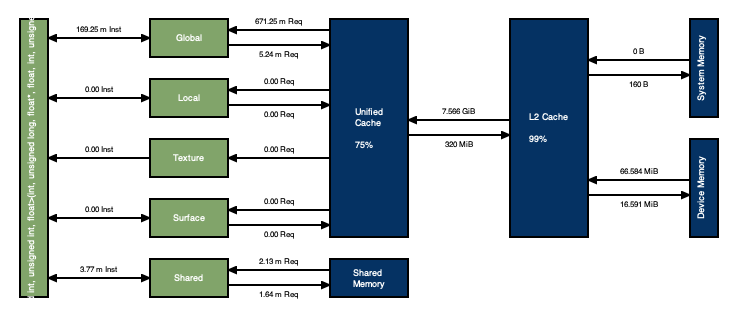
\includegraphics{attachments/sage/pokec_TitanXp.png}
\caption{Sage\_Pokec\_TianXp}
\end{figure}

It's clear that the unified cache is almost fully utilized, at 4 TBps
out of the 5 TBps theoretical upper bound, and is the bottleneck. This
is because the \texttt{W} arrays and the intermediate arrays are highly
reusable.

Running the same experiment on the V100 shows a different picture within
the memory system:

\begin{longtable}[]{@{}lrrl@{}}
\toprule
Type & Transactions & Bandwidth & Utilization\tabularnewline
\midrule
\endhead
Shared Loads & 2138599 & 74.166 GB/s &\tabularnewline
Shared Stores & 1640842 & 56.904 GB/s &\tabularnewline
Shared Total & 3779441 & 131.070 GB/s & Idle to low\tabularnewline
Local Loads & 0 & 0 GB/s &\tabularnewline
Local Stores & 0 & 0 GB/s &\tabularnewline
Global Loads & 419594240 & 3637.862 GB/s &\tabularnewline
Global Stores & 0 & 0 GB/s &\tabularnewline
Texture Reads & 177448960 & 6153.897 GB/s &\tabularnewline
Unified Total & 597043200 & 9791.759 GB/s & Medium\tabularnewline
L2 Reads & 8209326 & 71.174 GB/s &\tabularnewline
L2 Writes & 5243176 & 45.458 GB/s &\tabularnewline
L2 Total & 274655965 & 116.633 GB/s & Idle to low\tabularnewline
Device Reads & 2402833 & 20.832 GB/s &\tabularnewline
Device Writes & 571925 & 4.959 GB/s &\tabularnewline
Device Total & 2974758 & 25.791 GB/s & Idle to low\tabularnewline
\bottomrule
\end{longtable}

\begin{figure}
\centering
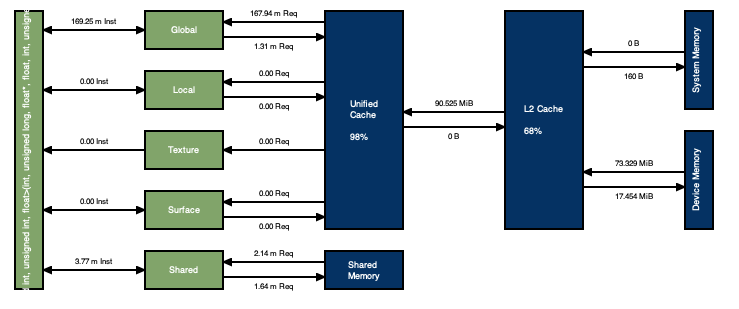
\includegraphics{attachments/sage/pokec_V100.png}
\caption{Sage\_Pokec\_V100}
\end{figure}

On the V100, kernel2 only takes 3.982 ms (about 60\% of 6.67 ms per
batch), and the unified-cache throughput increases to 9.8 TBps, more
than double than on the Titan Xp. In fact, the theoretical upper bound
of V100's L1 throughput is 28 TBps, resulted from doubling each SM's
load throughput from 128 bytes per cycle to 256 bytes per cycle, and
increasing the SM count to 80. This is the reason why the V100 can
outperform P100 and Titan Xp by about 3X. The performance bottleneck is
no longer the memory system, and switches to integer computations, which
comes mainly from array index calculation. This particular kernel also
takes up 32 registers per thread, which is the limit for full GPU
occupancy. Storing intermediate index calculation results would help if
the register usage is not so high.

\hypertarget{next-steps-2}{%
\section{Next Steps}\label{next-steps-2}}

\hypertarget{alternate-approaches-1}{%
\subsection{Alternate approaches}\label{alternate-approaches-1}}

\textbf{Things we tried that didn't really work}

An simple implementation that uses a thread to process the per-source or
per-child computation is coded, but it runs about 10X slower than the
current implementation that uses a block to process such units. One
reason is the use of block-level parallel primitives, such as block
reduce. Another reason is that by using a whole block, instead of a
thread, to process the same computation, the working set is greatly
reduced together with the parallelism, and the whole working set can fit
into the cache system. When using higher parallelism, the working set is
larger, and forced to be evicted into the global memory, and creates a
bottleneck. Actually during the experiment, for the thread-level
parallelism implementation, reducing the number of blocks of the kernel
improves its running time, the opposite to normally what would be
expected from running other kernels.

\hypertarget{gunrock-implications-1}{%
\subsection{Gunrock implications}\label{gunrock-implications-1}}

One thing that Gunrock does not provide, or intentionally hides, is
block-level parallelism. However, it comes in handy when implementing
the custom kernels for GraphSAGE: each block can process a one-dimension
vector, with each thread holding one element, then use a block-level
reduce to get the sum of those elements; this way is highly efficient,
and actually reduces the parallelism and with it the size of the working
set of data.

\hypertarget{notes-on-multi-gpu-parallelization-2}{%
\subsection{Notes on multi-GPU
parallelization}\label{notes-on-multi-gpu-parallelization-2}}

The main memory usage is due to feature data, so it is critical to not
duplicate features. The side effect is the computation needs to be
divided into child-centric and source-centric parts, and exchange data
in between. It should be scalable, and easy to implement.

\hypertarget{notes-on-dynamic-graphs-2}{%
\subsection{Notes on dynamic graphs}\label{notes-on-dynamic-graphs-2}}

GraphSAGE does not have a dynamic graph component, but it should able to
work on a dynamic graph. Some of the data may be reusable if the graph
has not been significantly changed, but the resulting memory requirement
to store the intermediate data may make data reuse impossible.

\hypertarget{notes-on-larger-datasets-2}{%
\subsection{Notes on larger datasets}\label{notes-on-larger-datasets-2}}

If the dataset is so large that the graph and the per-vertex feature
data are larger than the combined GPU memory, it's possible to
accumulate the features of leafs and children on CPU, transfer the data
on to GPU, and perform the computation. Because of the cost of the
transfer, runtime will increase significantly as compared to the cases
when the full data can fit in the GPU memory, but whether that will
cause an increase above the OpenMP implementation is still unknown.

\hypertarget{notes-on-other-pieces-of-this-workload-2}{%
\subsection{Notes on other pieces of this
workload}\label{notes-on-other-pieces-of-this-workload-2}}

The main part of GraphSAGE workflow is actually the training process,
which will be outside of Gunrock, provided by TensorFlow, PyTorch or
other machine learning libraries. How to connect the training with the
Gunrock GPU implementation is the main task for this workload going
forward.

\hypertarget{research-potential-1}{%
\subsection{Research potential}\label{research-potential-1}}

The GPU implementation of the embedding part runs a lot faster than on
the CPU, and hits a few GPU hardware limitations. It should have
comparable runtime to other GPU implementations. But it's only useful as
a part of the whole workload and achieves comparable prediction accuracy
as conventional / reference implementations.

An interesting question raised from the GraphSAGE GPU implementation is
whether it is useful to expose block-level parallelism to higher-level
programming models/APIs, and if so, how to do that. It's clear that
working at the block level provides benefits, such as the ability to use
block-level primitives like scan and reduce. But it also comes with
costs, most importantly, requiring the programmer to have knowledge
about the GPU hardware. It also reduces the portability of the
implementation, because two-level parallelism may not exist on other
processors.

\hypertarget{graphsearch-1}{%
\chapter{GraphSearch}\label{graphsearch-1}}

The graph search (GS) workflow is a walk-based method that searches a
graph for nodes that score highly on some arbitrary indicator of
interest.

The use case given by the HIVE government partner was sampling a graph:
given some seed nodes, and some model that can score a node as
``interesting'', find lots of ``interesting'' nodes as quickly as
possible. Their algorithm attempts to solve this problem by implementing
several different strategies for walking the graph.

\begin{itemize}
\tightlist
\item
  \texttt{uniform}: given a node \texttt{u}, randomly move to one of
  \texttt{u}'s neighbors (ignoring scores)
\item
  \texttt{greedy}: given a node \texttt{u}, walk to neighbor with
  maximum score
\item
  \texttt{stochastic\_greedy}: given a node \texttt{u}, choose neighbor
  to walk to with probability proportional to score
\end{itemize}

Use of these walk-based methods is motivated by the presence of
homophily in many real world social networks: we expect interesting
people to have relationships with interesting people.

\hypertarget{summary-of-results-3}{%
\section{Summary of Results}\label{summary-of-results-3}}

Graph search is a relatively minor modification to Gunrock's random walk
application, and was straightforward to implement. Though random walks
are a ``worst case scenario'' for GPU memory bandwidth, we still achieve
3--5x speedup over a modified version of the OpenMP reference
implementation.

The original OpenMP reference implementation actually ran slower with
more threads -- we fixed the bugs, but the benchmarking experience
highlights the need for performant and hardened CPU baselines.

Until recently, Gunrock did not support parallelism \emph{within} the
lambda functions run by the \texttt{advance} operator, so neighbor
selection for a given step in the walk is done sequentially. Methods for
exposing more parallelism to the programmer are currently being
developed via parallel neighbor reduce functions.

In an end-to-end graph search application, we'd need to implement the
scoring function as well as the graph walk component. For performance,
we'd likely want to implement the scoring function on the GPU as well,
which makes this a good example of a ``Gunrock+X'' app, where we'd need
to integrate the high-performance graph processing component with
arbitrary user code.

\hypertarget{summary-of-gunrock-implementation-2}{%
\section{Summary of Gunrock
Implementation}\label{summary-of-gunrock-implementation-2}}

The scoring model can be an arbitrary function (e.g., of node metadata).
For example, if we were running GS on the Twitter friends/followers
graph, the scoring model might be the output of a text classifier on
each users' messages. Thus, we do not implement the scoring model in our
Gunrock implementation -- instead, we read scores from an input file and
access them as necessary.

GS is a generalization of a random walk implementation, where there can
be more variety in the transition function between nodes.

The GS \texttt{uniform} mode is exactly a uniform random walk, so we can
use the pre-existing Gunrock application. Given a node, we compute the
node to walk to as:

\begin{Shaded}
\begin{Highlighting}[]
\NormalTok{r }\OperatorTok{=}\NormalTok{ random.uniform(}\DecValTok{0}\NormalTok{, }\DecValTok{1}\NormalTok{)}
\NormalTok{neighbors }\OperatorTok{=}\NormalTok{ graph.get_neighbors(node)}
\NormalTok{next_node }\OperatorTok{=}\NormalTok{ neighbors[floor(r }\OperatorTok{*} \BuiltInTok{len}\NormalTok{(neighbors))]}
\end{Highlighting}
\end{Shaded}

Both the \texttt{GraphSearch} \texttt{greedy} and
\texttt{stochastic\_greedy} consist of small modifications to this
transition function.

For \texttt{greedy}, we find the neighbor with maximum score:

\begin{Shaded}
\begin{Highlighting}[]
\NormalTok{neighbors }\OperatorTok{=}\NormalTok{ graph.get_neighbors(node)}
\NormalTok{next_node }\OperatorTok{=}\NormalTok{ neighbors[}\DecValTok{0}\NormalTok{]}
\NormalTok{next_node_score }\OperatorTok{=}\NormalTok{ scores[next_node]}
\ControlFlowTok{for}\NormalTok{ neighbor }\KeywordTok{in}\NormalTok{ neighbors:}
\NormalTok{    neighbor_score }\OperatorTok{=}\NormalTok{ scores[neighbor]}
    \ControlFlowTok{if}\NormalTok{ neighbor_score }\OperatorTok{>}\NormalTok{ next_node_score:}
\NormalTok{        next_node }\OperatorTok{=}\NormalTok{ neighbor}
\NormalTok{        next_node_score }\OperatorTok{=}\NormalTok{ neighbor_score}
\end{Highlighting}
\end{Shaded}

For \texttt{stochastic\_greedy}, we sample neighbors proportional to
their score -- e.g.:

\begin{Shaded}
\begin{Highlighting}[]
\NormalTok{sum_neighbor_scores }\OperatorTok{=} \DecValTok{0}
\ControlFlowTok{for}\NormalTok{ neighbor }\KeywordTok{in}\NormalTok{ graph.neighbors(node):}
\NormalTok{   sum_neighbor_scores }\OperatorTok{+=}\NormalTok{ scores[neighbor]}

\NormalTok{r }\OperatorTok{*=}\NormalTok{ sum_neighbor_scores}

\NormalTok{tmp }\OperatorTok{=} \DecValTok{0}
\ControlFlowTok{for}\NormalTok{ neighbor }\KeywordTok{in}\NormalTok{ graph.neighbors(node):}
\NormalTok{   tmp }\OperatorTok{+=}\NormalTok{ scores[neighbor]}
   \ControlFlowTok{if}\NormalTok{ r }\OperatorTok{<}\NormalTok{ tmp:}
\NormalTok{       next_node }\OperatorTok{=}\NormalTok{ neighbor}
       \ControlFlowTok{break}
\end{Highlighting}
\end{Shaded}

In Gunrock, we create a frontier containing all of the nodes we want to
walk from. Then we map the transition function over the frontier using
Gunrock's \texttt{ForEach} operator. Current nodes in the frontier are
replaced with the chosen neighbor, and the walk is (optionally) recorded
in an output array.

Because this is such a straightforward modification, we implement GS
inside of the existing random walk \texttt{rw} Gunrock application. GS
just requires adding a couple of extra flags and one extra array of size
\texttt{\textbar{}V\textbar{}} to store the node values.

\hypertarget{how-to-run-this-application-on-darpas-dgx-1-3}{%
\section{How To Run This Application on DARPA's
DGX-1}\label{how-to-run-this-application-on-darpas-dgx-1-3}}

\hypertarget{prereqsinput-2}{%
\subsection{Prereqs/input}\label{prereqsinput-2}}

\begin{Shaded}
\begin{Highlighting}[]
\FunctionTok{git}\NormalTok{ clone --recursive https://github.com/gunrock/gunrock -b dev-refactor}
\BuiltInTok{cd}\NormalTok{ gunrock/tests/rw/}
\FunctionTok{cp}\NormalTok{ ../../gunrock/util/gitsha1.c.in ../../gunrock/util/gitsha1.c}
\FunctionTok{make}\NormalTok{ clean}
\FunctionTok{make}
\end{Highlighting}
\end{Shaded}

\hypertarget{running-the-application-3}{%
\subsection{Running the application}\label{running-the-application-3}}

\hypertarget{application-specific-parameters-1}{%
\subsubsection{Application specific
parameters}\label{application-specific-parameters-1}}

\begin{verbatim}
  --walk-mode
      0 = uniform
      1 = greedy
      2 = stochastic_greedy
  --node-value-path
      If --walk-mode != 0, this is the path to node scores
  --store-walks
      0 = just do the walk -- don't actually store it anywhere
      1 = store walks in memory
  --walk-length
      Length of each walk
  --walks-per-node
      Number of walks to do per seed node
  --seed
      Seed for random number generator
\end{verbatim}

\hypertarget{example-command-2}{%
\subsubsection{Example Command}\label{example-command-2}}

\begin{Shaded}
\begin{Highlighting}[]
\CommentTok{# generate random features}
\ExtensionTok{python}\NormalTok{ random-values.py 39 }\OperatorTok{>}\NormalTok{ chesapeake.values}

\CommentTok{# uniform random}
\ExtensionTok{./bin/test_rw_9.1_x86_64}\NormalTok{ --graph-type market --graph-file \textbackslash{}}
\NormalTok{  ../../dataset/small/chesapeake.mtx --walk-mode 0 --seed 123}

\CommentTok{# greedy}
\ExtensionTok{./bin/test_rw_9.1_x86_64}\NormalTok{ --graph-type market --graph-file \textbackslash{}}
\NormalTok{  ../../dataset/small/chesapeake.mtx --node-value-path chesapeake.values \textbackslash{}}
\NormalTok{  --walk-mode 1}

\CommentTok{# stochastic greedy}
\ExtensionTok{./bin/test_rw_9.1_x86_64}\NormalTok{ --graph-type market --graph-file \textbackslash{}}
\NormalTok{  ../../dataset/small/chesapeake.mtx --node-value-path chesapeake.values \textbackslash{}}
\NormalTok{  --walk-mode 2 --seed 123}
\end{Highlighting}
\end{Shaded}

\hypertarget{example-output-1}{%
\subsubsection{Example Output}\label{example-output-1}}

\begin{verbatim}
# ------------------------------------------------
# uniform random

Loading Matrix-market coordinate-formatted graph ...
Reading from ../../dataset/small/chesapeake.mtx:
  Parsing MARKET COO format
 (39 nodes, 340 directed edges)...
Done parsing (0 s).
  Converting 39 vertices, 340 directed edges ( ordered tuples) to CSR format...
Done converting (0s).
__________________________
--------------------------
 Elapsed: 0.001907
Using advance mode LB
Using filter mode CULL
num_nodes=39
__________________________
0    0   0   queue3      oversize :  234 ->  682
0    0   0   queue3      oversize :  234 ->  682
0    1   0   queue3      oversize :  682 ->  1085
0    1   0   queue3      oversize :  682 ->  1085
0    5   0   queue3      oversize :  1085 ->     1166
0    5   0   queue3      oversize :  1085 ->     1166
--------------------------
Run 0 elapsed: 4.551888, #iterations = 10
[[0, 38, 8, 35, 11, 25, 13, 27, 37, 7, ],
[1, 34, 1, 38, 30, 38, 29, 37, 7, 37, ],
[2, 17, 2, 38, 4, 38, 10, 18, 14, 28, ],
...
[36, 33, 0, 22, 38, 27, 37, 18, 38, 8, ],
[37, 21, 31, 17, 25, 17, 18, 32, 37, 26, ],
[38, 7, 8, 34, 6, 5, 6, 5, 38, 19, ]]
-------- NO VALIDATION -----[rw] finished.
 avg. elapsed: 4.551888 ms
 iterations: 10
 min. elapsed: 4.551888 ms
 max. elapsed: 4.551888 ms
 load time: 60.925 ms
 preprocess time: 964.890000 ms
 postprocess time: 0.715017 ms
 total time: 970.350027 ms

# ------------------------------------------------
# greedy
# !! In this case, the output is formatted as `GPU_result:CPU_result`, for correctness checking

Loading Matrix-market coordinate-formatted graph ...
Reading from ../../dataset/small/chesapeake.mtx:
  Parsing MARKET COO format
 (39 nodes, 340 directed edges)...
Done parsing (0 s).
  Converting 39 vertices, 340 directed edges ( ordered tuples) to CSR format...
Done converting (0s).
__________________________
--------------------------
 Elapsed: 0.085831
Using advance mode LB
Using filter mode CULL
num_nodes=39
__________________________
0    0   0   queue3      oversize :  234 ->  682
0    0   0   queue3      oversize :  234 ->  682
0    1   0   queue3      oversize :  682 ->  770
0    1   0   queue3      oversize :  682 ->  770
--------------------------
Run 0 elapsed: 0.695944, #iterations = 10
[[0:0, 22:22, 32:32, 18:18, 11:11, 18:18, 11:11, 18:18, 11:11, 18:18, ],
[1:1, 22:22, 32:32, 18:18, 11:11, 18:18, 11:11, 18:18, 11:11, 18:18, ],
[2:2, 17:17, 2:2, 17:17, 2:2, 17:17, 2:2, 17:17, 2:2, 17:17, ],
...
[36:36, 33:33, 36:36, 33:33, 36:36, 33:33, 36:36, 33:33, 36:36, 33:33, ],
[37:37, 18:18, 11:11, 18:18, 11:11, 18:18, 11:11, 18:18, 11:11, 18:18, ],
[38:38, 2:2, 17:17, 2:2, 17:17, 2:2, 17:17, 2:2, 17:17, 2:2, ]]
0 errors occurred.
[rw] finished.
 avg. elapsed: 0.695944 ms
 iterations: 10
 min. elapsed: 0.695944 ms
 max. elapsed: 0.695944 ms
 load time: 44.2419 ms
 preprocess time: 974.721000 ms
 postprocess time: 0.731945 ms
 total time: 976.338863 ms

# ------------------------------------------------
# stochastic_greedy
# Output same format as `uniform` above.
# No correctness checking is implemented due to stochasticity.
\end{verbatim}

\hypertarget{expected-output-1}{%
\subsubsection{Expected Output}\label{expected-output-1}}

When run in \texttt{-\/-verbose} mode, the app outputs the walks. When
run in \texttt{-\/-quiet} mode, it outputs performance statistics (e.g.,
total number of steps taken). If running \texttt{greedy}
\texttt{GraphSearch}, the app also outputs the results of a correctness
check. Correctness checks for \texttt{uniform} and
\texttt{stochastic\_greedy} are omitted because of their inherent
stochasticity.

\hypertarget{validation}{%
\subsection{Validation}\label{validation}}

The correctness of the implementation has been validated in outside
experiments, by making sure that the output walks are valid and the
distribution of transitions is as expected.

\hypertarget{performance-and-analysis-3}{%
\section{Performance and Analysis}\label{performance-and-analysis-3}}

Performance is measured by the runtime of the app, given

\begin{itemize}
\tightlist
\item
  an input graph \texttt{G=(U,\ E)}
\item
  set of seed nodes (hardcoded to all nodes in \texttt{G})
\item
  number of walks per seed
\item
  number of steps per walk
\item
  a transition function (e.g.,
  \texttt{uniform\textbar{}greedy\textbar{}stochastic\_greedy})
\end{itemize}

\hypertarget{implementation-limitations-3}{%
\subsection{Implementation
limitations}\label{implementation-limitations-3}}

The output of the random walk is a dense array of size
\texttt{(\#\ seeds)\ *\ (steps\ per\ walk)\ *\ (walks\ per\ seed)}. When
we have a large graph \emph{or} long walks \emph{or} multiple walks per
seed, this array may exceed the size of GPU memory.

At the moment, we only support walks starting from \emph{all} of the
nodes in \texttt{G}. It would be straightforward to add a parameter that
would allow the use to specify a smaller set of seed nodes.

This app can only be used for graphs that have scores associated w/ each
node. In order to run benchmarks, if scores are not available we often
assign uniformly random scores to nodes. The distribution of these
scores may affect the runtime of the algorithm by changing data access
patterns -- we test on the provided Twitter dataset, but do not have a
variety of other node attributed graphs to test on.

\hypertarget{comparison-against-existing-implementations-3}{%
\subsection{Comparison against existing
implementations}\label{comparison-against-existing-implementations-3}}

We measure runtime on the
\href{https://hiveprogram.com/data/_v0/graph_search/}{HIVE graphsearch
Twitter dataset}. This graph has \texttt{\textbar{}U\textbar{}=9291392}
nodes and \texttt{\textbar{}E\textbar{}=21741663} edges.

At a high level, the results show:

\begin{longtable}[]{@{}llll@{}}
\toprule
Variant & OpenMP w/ 64 threads & Gunrock GPU & Gunrock
Speedup\tabularnewline
\midrule
\endhead
Directed greedy & 236ms & \textbf{64ms} & 3.7x\tabularnewline
Directed random & 158ms & \textbf{34ms} & 4.6x\tabularnewline
Undirected random & 3186ms & \textbf{630ms} & 5.0x\tabularnewline
\bottomrule
\end{longtable}

The undirected random walks take \textasciitilde{} 10x longer because
directed walks terminate when they encounter a node without any
neighbors and thus have average length significantly shorter than the
\texttt{-\/-walk-length} parameter.

Details and raw data follow.

\hypertarget{hive-python-reference-implementation}{%
\subsubsection{HIVE Python reference
implementation}\label{hive-python-reference-implementation}}

We run the HIVE Python reference implementation w/ the following
settings:

\begin{itemize}
\tightlist
\item
  undirected graph
\item
  uniform transition function
\item
  1000 random seeds
\item
  128 steps per walk
\end{itemize}

With the \texttt{uniform} transition function, the run took 41 seconds.
Walks are done sequentially, so runtime will scale linearly with the
number of seeds. This implementation is \emph{substantially} slower than
even a single-threaded run of PNNLs OpenMP code. Thus, we omit further
analysis.

\hypertarget{pnnl-openmp-implementation}{%
\subsubsection{PNNL OpenMP
implementation}\label{pnnl-openmp-implementation}}

We run the PNNL OpenMP implementation on the Twitter graph w/ the
following settings:

\begin{itemize}
\tightlist
\item
  commit: 69864383f0fc0e8aace52be34b329a2f8a58afb6
\item
  1,2,4,8,16,32 or 64 threads
\item
  \texttt{greedy} or \texttt{uniform} transition function
\item
  directed or undirected graph
\end{itemize}

We omit the \texttt{greedy} undirected case because the algorithm gets
stuck jumping between a local maximum and its highest-scoring neighbor.

\begin{longtable}[]{@{}lllllll@{}}
\toprule
threads & method & directed? & nseeds & elapsed\_sec & nsteps &
steps\_per\_sec\tabularnewline
\midrule
\endhead
1 & greedy & yes & 7199978 & 3.02876 & 16325873 &
5.39e+06\tabularnewline
2 & greedy & yes & 7199978 & 2.83467 & 16325873 &
5.75e+06\tabularnewline
4 & greedy & yes & 7199978 & 1.64405 & 16325873 &
9.93e+06\tabularnewline
8 & greedy & yes & 7199978 & 0.870028 & 16325873 &
1.87e+07\tabularnewline
16 & greedy & yes & 7199978 & 0.605769 & 16325873 &
2.69e+07\tabularnewline
32 & greedy & yes & 7199978 & 0.43742 & 16325873 &
3.73e+07\tabularnewline
64 & greedy & yes & 7199978 & \textbf{0.236701} & 16325873 &
6.89e+07\tabularnewline
1 & unif. & yes & 7199978 & \textbf{14.6291} & 14510781 &
\textbf{991915}\tabularnewline
2 & unif. & yes & 7199978 & 24.2175 & 14186833 & 585809\tabularnewline
4 & unif. & yes & 7199978 & 25.1764 & 14487202 & 575427\tabularnewline
8 & unif. & yes & 7199978 & 27.7312 & 13937449 & 502591\tabularnewline
16 & unif. & yes & 7199978 & 30.5377 & 14062226 & 460488\tabularnewline
32 & unif. & yes & 7199978 & 32.1057 & 13906144 & 433137\tabularnewline
64 & unif. & yes & 7199978 & 31.2754 & 13876284 & 443680\tabularnewline
1 & unif. & no & 100000 & \textbf{12.3982} & 12700000 &
\textbf{1.024+06}\tabularnewline
2 & unif. & no & 100000 & 19.7925 & 12700000 & 641658\tabularnewline
4 & unif. & no & 100000 & 22.5432 & 12700000 & 563362\tabularnewline
8 & unif. & no & 100000 & 26.1053 & 12700000 & 486491\tabularnewline
16 & unif. & no & 100000 & 28.275 & 12700000 & 449160\tabularnewline
32 & unif. & no & 100000 & 28.334 & 12700000 & 448224\tabularnewline
64 & unif. & no & 100000 & 28.7419 & 12700000 & 441864\tabularnewline
\bottomrule
\end{longtable}

Note that we use fewer seeds for the undirected uniform case due to slow
runtime.

Observe that the \texttt{rand} modes have very bad scaling as a function
of cores. After investigation, this was due to two issues. First, the
neighbors were being sampled incorrectly, which led to chaotic behavior.
Second, the app was using a slow random number generator w/ an excessive
number of seed resets. We created a PR to fix those issues
\href{https://gitlab.hiveprogram.com/pnnl/graphsearch/merge_requests/1}{here}.

After these fixes, runtimes were as follows:

\begin{longtable}[]{@{}lllllll@{}}
\toprule
threads & method & directed? & nseeds & elapsed\_sec & nsteps &
steps\_per\_sec\tabularnewline
\midrule
\endhead
1 & greedy & yes & 7199978 & 3.02876 & 16325873 &
5.39e+06\tabularnewline
2 & greedy & yes & 7199978 & 2.83467 & 16325873 &
5.75e+06\tabularnewline
4 & greedy & yes & 7199978 & 1.64405 & 16325873 &
9.93e+06\tabularnewline
8 & greedy & yes & 7199978 & 0.870028 & 16325873 &
1.87e+07\tabularnewline
16 & greedy & yes & 7199978 & 0.605769 & 16325873 &
2.69e+07\tabularnewline
32 & greedy & yes & 7199978 & 0.43742 & 16325873 &
3.73e+07\tabularnewline
64 & greedy & yes & 7199978 & \textbf{0.236701} & 16325873 &
\textbf{6.89e+07}\tabularnewline
1 & unif. & yes & 7199978 & 1.49886 & 16529694 & 1.10e+07\tabularnewline
2 & unif. & yes & 7199978 & 1.60176 & 16533004 & 1.03e+07\tabularnewline
4 & unif. & yes & 7199978 & 0.974128 & 16538957 &
1.69e+07\tabularnewline
8 & unif. & yes & 7199978 & 0.455227 & 16534756 & 3.63+07\tabularnewline
16 & unif. & yes & 7199978 & 0.257524 & 16528617 &
6.42e+07\tabularnewline
32 & unif. & yes & 7199978 & \textbf{0.155722} & 13906144 &
\textbf{1.06e+08}\tabularnewline
64 & unif. & yes & 7199978 & 0.158828 & 16537488 &
1.04e+08\tabularnewline
1 & unif. & no & 7199978 & 125.963 & 914397206 & 1.92e+08\tabularnewline
2 & unif. & no & 7199978 & 78.927 & 914397206 & 1.80e+08\tabularnewline
4 & unif. & no & 7199978 & 39.7097 & 914397206 & 2.96e+08\tabularnewline
8 & unif. & no & 7199978 & 22.5195 & 914397206 & 6.35e+08\tabularnewline
16 & unif. & no & 7199978 & 11.0047 & 914397206 &
1.12e+09\tabularnewline
32 & unif. & no & 7199978 & 5.56317 & 914397206 &
\textbf{1.85e+09}\tabularnewline
64 & unif. & no & 7199978 & \textbf{3.18615} & 914397206 &
1.82e+09\tabularnewline
\bottomrule
\end{longtable}

Note the improved runtimes and scaling. These experiments were run with
\href{https://gitlab.hiveprogram.com/bjohnson/graphsearch/tree/gunrock_test}{this
branch} at commit 6c25a0687eecebfd4393e86fa4c7308d5594b73d.

All experiments are conducted on the HIVE DGX-1.

\hypertarget{gunrock-gpu-implementation}{%
\subsubsection{Gunrock GPU
implementation}\label{gunrock-gpu-implementation}}

\hypertarget{directed-greedy}{%
\subparagraph{directed, greedy}\label{directed-greedy}}

\begin{Shaded}
\begin{Highlighting}[]
\ExtensionTok{./bin/test_rw_9.1_x86_64}\NormalTok{ --graph-type market --graph-file dir_gs_twitter.mtx \textbackslash{}}
\NormalTok{    --node-value-path gs_twitter.values \textbackslash{}}
\NormalTok{    --walk-mode 1 \textbackslash{}}
\NormalTok{    --walk-length 32 \textbackslash{}}
\NormalTok{    --undirected=0 \textbackslash{}}
\NormalTok{    --store-walks 0 \textbackslash{}}
\NormalTok{    --quick \textbackslash{}}
\NormalTok{    --num-runs 10}
\end{Highlighting}
\end{Shaded}

\begin{verbatim}
Loading Matrix-market coordinate-formatted graph ...
Reading from dir_gs_twitter.mtx:
  Parsing MARKET COO format
 (7199978 nodes, 21741663 directed edges)...
Done parsing (7 s).
  Converting 7199978 vertices, 21741663 directed edges ( ordered tuples) to CSR format...
Done converting (0s).
==============================================
 advance-mode=LB
Using advance mode LB
Using filter mode CULL
Run 0 elapsed: 65.273046, #iterations = 32
Run 1 elapsed: 64.157963, #iterations = 32
Run 2 elapsed: 64.009190, #iterations = 32
Run 3 elapsed: 64.055920, #iterations = 32
Run 4 elapsed: 64.069033, #iterations = 32
Run 5 elapsed: 64.002037, #iterations = 32
Run 6 elapsed: 64.031839, #iterations = 32
Run 7 elapsed: 64.036846, #iterations = 32
Run 8 elapsed: 64.065933, #iterations = 32
Run 9 elapsed: 64.047098, #iterations = 32
Validate_Results: total_neighbors_seen=298668024
Validate_Results: total_steps_taken=16325873
-------- NO VALIDATION --------
[rw] finished.
 avg. elapsed: 64.174891 ms
 iterations: 32
 min. elapsed: 64.002037 ms
 max. elapsed: 65.273046 ms
 load time: 7086.91 ms
 preprocess time: 1016.620000 ms
 postprocess time: 101.121902 ms
 total time: 2073.837996 ms
\end{verbatim}

\hypertarget{directed-uniform}{%
\subparagraph{directed, uniform}\label{directed-uniform}}

\begin{Shaded}
\begin{Highlighting}[]
\ExtensionTok{./bin/test_rw_9.1_x86_64}\NormalTok{ --graph-type market --graph-file dir_gs_twitter.mtx \textbackslash{}}
\NormalTok{    --node-value-path gs_twitter.values \textbackslash{}}
\NormalTok{    --walk-mode 0 \textbackslash{}}
\NormalTok{    --walk-length 128 \textbackslash{}}
\NormalTok{    --undirected=0 \textbackslash{}}
\NormalTok{    --store-walks 0 \textbackslash{}}
\NormalTok{    --quick \textbackslash{}}
\NormalTok{    --num-runs 10 \textbackslash{}}
\NormalTok{    --seed 123}
\end{Highlighting}
\end{Shaded}

\begin{verbatim}
Loading Matrix-market coordinate-formatted graph ...
Reading from dir_gs_twitter.mtx:
  Parsing MARKET COO format
 (7199978 nodes, 21741663 directed edges)...
Done parsing (7 s).
  Converting 7199978 vertices, 21741663 directed edges ( ordered tuples) to CSR format...
Done converting (1s).
==============================================
 advance-mode=LB
Using advance mode LB
Using filter mode CULL
__________________________
Run 0 elapsed: 38.613081, #iterations = 128
Run 1 elapsed: 34.458876, #iterations = 128
Run 2 elapsed: 34.530163, #iterations = 128
Run 3 elapsed: 33.849001, #iterations = 128
Run 4 elapsed: 33.759117, #iterations = 128
Run 5 elapsed: 33.967972, #iterations = 128
Run 6 elapsed: 33.873081, #iterations = 128
Run 7 elapsed: 33.970118, #iterations = 128
Run 8 elapsed: 33.756971, #iterations = 128
--------------------------
Run 9 elapsed: 33.715963, #iterations = 128
Validate_Results: total_neighbors_seen=289124779
Validate_Results: total_steps_taken=16530404
-------- NO VALIDATION --------
[rw] finished.
 avg. elapsed: 34.449434 ms
 iterations: 128
 min. elapsed: 33.715963 ms
 max. elapsed: 38.613081 ms
 load time: 7176.17 ms
 preprocess time: 1016.720000 ms
 postprocess time: 101.902962 ms
 total time: 1781.071901 ms
\end{verbatim}

\hypertarget{undirected-uniform}{%
\subparagraph{undirected, uniform}\label{undirected-uniform}}

\begin{Shaded}
\begin{Highlighting}[]
\ExtensionTok{./bin/test_rw_9.1_x86_64}\NormalTok{ --graph-type market --graph-file undir_gs_twitter.mtx \textbackslash{}}
\NormalTok{    --node-value-path gs_twitter.values \textbackslash{}}
\NormalTok{    --walk-mode 0 \textbackslash{}}
\NormalTok{    --walk-length 128 \textbackslash{}}
\NormalTok{    --store-walks 0 \textbackslash{}}
\NormalTok{    --quick \textbackslash{}}
\NormalTok{    --num-runs 10 \textbackslash{}}
\NormalTok{    --seed 123}
\end{Highlighting}
\end{Shaded}

\begin{verbatim}
Loading Matrix-market coordinate-formatted graph ...
Reading from undir_gs_twitter.mtx:
  Parsing MARKET COO format
 (7199978 nodes, 43483326 directed edges)...
Done parsing (7 s).
  Converting 7199978 vertices, 43483326 directed edges ( ordered tuples) to CSR format...
Done converting (0s).
==============================================
 advance-mode=LB
Using advance mode LB
Using filter mode CULL
Run 0 elapsed: 636.021852, #iterations = 128
Run 1 elapsed: 631.129026, #iterations = 128
Run 2 elapsed: 631.053925, #iterations = 128
Run 3 elapsed: 631.713152, #iterations = 128
Run 4 elapsed: 631.028175, #iterations = 128
Run 5 elapsed: 631.374836, #iterations = 128
Run 6 elapsed: 631.196976, #iterations = 128
Run 7 elapsed: 632.030964, #iterations = 128
Run 8 elapsed: 631.026983, #iterations = 128
Run 9 elapsed: 630.996943, #iterations = 128
Validate_Results: total_neighbors_seen=75443835041
Validate_Results: total_steps_taken=914397206
-------- NO VALIDATION --------
[rw] finished.
 avg. elapsed: 631.757283 ms
 iterations: 128
 min. elapsed: 630.996943 ms
 max. elapsed: 636.021852 ms
 load time: 7705.9 ms
 preprocess time: 1010.830000 ms
 postprocess time: 102.057934 ms
 total time: 7755.448818 ms
\end{verbatim}

\hypertarget{performance-limitations-3}{%
\subsection{Performance limitations}\label{performance-limitations-3}}

\begin{itemize}
\tightlist
\item
  For the undirected uniform settings, profiling shows that 79\% of
  compute time is spent in the \texttt{ForAll} operator and 20\% is
  spent in the \texttt{curand} random number generator. Device memory
  bandwidth in the \texttt{ForAll} kernel is 193 GB/s.
\item
  For the directed greedy settings, profiling shows that 99.5\% of
  compute time is spent in the \texttt{ForAll} operator. Device memory
  bandwidth in the \texttt{ForAll} kernel is 136 GB/s.
\end{itemize}

When we do a large number of walks and/or the length of each walk is
very long, there may not be enough GPU memory to store all of the walks
in memory. For now, we expose the \texttt{-\/-store-walks} parameter --
when this is set to zero, the walk is discarded as it is computed and
only the length of the walk is stored. A better solution that could be
implemented in the future would be to move walks from GPU to CPU memory
as they grow too large.

\textbf{Optimization:} In a directed walk, once we hit a node with no
outgoing neighbors, we halt the walk. In the current Gunrock
implementation, the enactor runs for a fixed number of iterations,
regardless of whether any of the nodes are still active. It would be
straightforward to add a check that terminates the app when no
``living'' nodes are left.

\hypertarget{next-steps-3}{%
\section{Next Steps}\label{next-steps-3}}

\hypertarget{alternate-approaches-2}{%
\subsection{Alternate approaches}\label{alternate-approaches-2}}

The size of the output array may become a significant bottleneck for
large graphs. However, since all of the transition functions do not
depend on anything besides the current node, we could reasonably move
the results of the walk from GPU to CPU memory every N iterations.
Properly executed, this should eliminate the largest bottleneck without
unduely impacting performance.

\hypertarget{gunrock-implications-2}{%
\subsection{Gunrock implications}\label{gunrock-implications-2}}

For the \texttt{greedy} and \texttt{stochastic\_greedy} transition
function, we have to sequentially iterate over all of a node's
neighbors. Simple wrappers for computing, e.g., the maximum of node
scores across all of a node's neighbors could be helpful, both for ease
of programming and performance. Gunrock has a newly added
\texttt{NeighborReduce} kernel that supports associative reductions --
it should be straightforward to implement (at least) the \texttt{greedy}
transition function with this kernel. The \texttt{stochastic\_greedy}
transition function would require a more complex reduction function
along the lines of reservoir sampling.

\hypertarget{notes-on-multi-gpu-parallelization-3}{%
\subsection{Notes on multi-GPU
parallelization}\label{notes-on-multi-gpu-parallelization-3}}

If the graph is small enough to be duplicated on each GPU, the
implementation is trivial: just do a subset of the walks on each GPU.
The scalability will be perfect, as there is no communication involved
at all.

When the graph is distributed across multiple GPUs, we expect to have
very poor scalability, as the ratio of computation to communication is
very low. A more detailed discussion is available
\href{https://gunrock.github.io/docs/hive_year1_summary.html\#scaling-analysis-for-hive-applications}{here}.

\hypertarget{notes-on-dynamic-graphs-3}{%
\subsection{Notes on dynamic graphs}\label{notes-on-dynamic-graphs-3}}

This workflow does not have an explicit dynamic component. However,
because steps only depend on the current node, the underlying graph
could change during the walks.

\hypertarget{notes-on-larger-datasets-3}{%
\subsection{Notes on larger datasets}\label{notes-on-larger-datasets-3}}

The random accesses inherent to graph search make it a particularly
difficult workflow for larger-than-GPU memory datasets. The most
straightforward solution would be to let Unified Virtual Memory (UVM) in
CUDA automatically handle memory movement, but we should expect to see a
substantial reduction in performance.

\hypertarget{notes-on-other-pieces-of-this-workload-3}{%
\subsection{Notes on other pieces of this
workload}\label{notes-on-other-pieces-of-this-workload-3}}

In real use cases, the scoring function would be computed lazily -- that
is, we wouldn't have a precomputed array with scores for each of the
nodes, and we would need to run the scoring function as the walk is
running. Thus, it would be critical for us to be able to call the
scoring function from within Gunrock quickly and without excessive
programmer overhead.

\hypertarget{community-detection-louvain-1}{%
\chapter{Community Detection
(Louvain)}\label{community-detection-louvain-1}}

Community detection in graphs means grouping vertices together, so that
those vertices that are closer (have more connections) to each other are
placed in the same cluster. A commonly used algorithm for community
detection is Louvain (\url{https://arxiv.org/pdf/0803.0476.pdf}).

\hypertarget{summary-of-results-4}{%
\section{Summary of Results}\label{summary-of-results-4}}

The Gunrock implementation uses sort and segmented reduce to implement
the Louvain algorithm, different from the commonly used hash table
mapping. The GPU implementation is about \textasciitilde{}1.5X faster
than the OpenMP implementation, and also faster than previous GPU works.
It is still unknown whether the sort and segmented reduce formulation
map the problem better than hash table on the GPU. The modularities
resulting from the GPU implementation are within small differences as
the serial implementation, and are better when the graph is larger. A
custom hash table can potentially improve the running time. The GPU
Louvain implementation should have moderate scalability across multiple
GPUs in an DGX-1.

\hypertarget{summary-of-gunrock-implementation-3}{%
\section{Summary of Gunrock
Implementation}\label{summary-of-gunrock-implementation-3}}

The commonly used approach to implement the Louvain algorithm uses a
hash table. However, the memory access pattern that results from a hash
table is almost totally random, and not GPU-friendly (more in the
Alternative approaches section). Instead of using a hash table to
accumulate the values associated with the same key, the Gunrock
implementation on GPU tries another method: sort all key-value pairs,
and use segmented reduce to accumulate the values in the continuous
segments. Because Louvain always visits all edges in the graph, there is
no need to use Gunrock frontiers, and the \texttt{advance} operator with
the \texttt{ALL\_EDGES} advance mode or a simple \texttt{ForAll} loop
should be sufficient. The pseudocode is listed below:

\begin{verbatim}
m2 <- sum(edge_weights);
//Outer-loop
Do
    // Pass-initialization, assign each vertex to its own community
    For each vertex v in graph:
        current_communities[v] <- v;
        weights_v2any      [v] <- 0;
        weights_v2self     [v] <- 0;
    For each edge e<v, u> in graph: //an advance operator on all edges
        weights_v2any[v] += edge_weights[e];
        if (v == u)
            weights_v2self[v] += edge_weights[e];
    For each vertex v in graph:
        weights_community2any[v] <- weights_v2any[v];
    pass_gain <- 0;

    // Modularity optimizing iterations
    Do
        // Get weights between vertex and community
        For each edge e<v, u> in graph:
            edge_pairs  [e] <- <v, current_communities[u]>;
            pair_weights[e] <- edge_weights[e];
        Sort(edge_pairs, pair_weights)
            by edge_pair.first, then edge_pair.second if tie;
        segment_offsets <- offsets of continuous edge_pairs;
        segment_weights <- SegmentedReduce(pair_weights, segment_offsets, sum);

        // Compute base modularity gains
        // if moving vertices out of current communities
        For each vertex v in graph:
            comm <- current_communities[v];
            w_v2comm <- Find weights from v to comm in segment_weights;
            gain_bases[v] = weights_v2self[v] - w_v2comm
                - (weights_v2any[v] - weights_community2any[comm])
                    * weights_v2any[v] / m2;

        // Find the max gains if moving vertices into adjacent communities
        For each vertex v in graph:
            gains[v] <- 0;
            next_communities[v] <- current_communities[v];
        For each seg<v, comm> segment:
            if (comm == current_communities[v])
                continue;
            gain <- gain_bases[v] + segment_weights[seg]
                - weights_community2any[comm] * weights_v2any[v] / m2;
            atomicMax(max_gains + v, gain);
            seg_gains[seg] <- gain;
        For each seg<v, comm> segment:
            if (seg_gains[seg] != max_gains[v])
                continue;
            next_communities[v] <- comm;

        // Update communities
        For each vertex v in graph:
            curr_comm <- current_communities[v];
            next_comm <- next_communities[v];
            if (curr_comm == next_comm)
                continue;

            atomicAdd(weights_community2any[next_comm],  weights_v2any[v]);
            atomicAdd(weights_community2any[curr_comm], -weights_v2any[v]);
            current_communities[v] <- next_comm;

        iteration_gain <- Reduce(max_gains, sum);
        pass_gain += iteration_gain;
    While iterations stop condition not met
    // End of modularity optimizing iterations

    // Contract the graph
    // renumber occupied communities
    new_communities <- Renumber(current_communities);
    For each edge e<v, u> in graph: //an advance operator on all edges
        edge_pairs[e] <- <new_communities[current_communities[v]],
                          new_communities[current_communities[u]]>
    Sort(edge_pairs, edge_weights) by pair.x, then pair.y if tie;
    segment_offsets <- offsets of continuous edge_pairs;
    new_graph.Allocate(|new_communities|, |segments|);
    new_graph.edges <- first pair of each segments;
    new_graph.edge_values <- SegmentedReduce(edge_weights, segment_offsets, sum);

While pass stop condition not met
\end{verbatim}

\hypertarget{how-to-run-this-application-on-darpas-dgx-1-4}{%
\section{How To Run This Application on DARPA's
DGX-1}\label{how-to-run-this-application-on-darpas-dgx-1-4}}

\hypertarget{prereqsinput-3}{%
\subsection{Prereqs/input}\label{prereqsinput-3}}

CUDA should have been installed; \texttt{\$PATH} and
\texttt{\$LD\_LIBRARY\_PATH} should have been set correctly to use CUDA.
The current Gunrock configuration assumes boost (1.58.0 or 1.59.0) and
Metis are installed; if not, changes need to be made in the Makefiles.
DARPA's DGX-1 has both installed when the tests are performed.

\begin{verbatim}
git clone --recursive https://github.com/gunrock/gunrock/
cd gunrock
git checkout dev-refactor
git submodule init
git submodule update
mkdir build
cd build
cmake ..
cd ../tests/louvain
make
\end{verbatim}

At this point, there should be an executable
\texttt{louvain\_main\_\textless{}CUDA\ version\textgreater{}\_x86\_64}
in \texttt{tests/louvain/bin}.

The datasets are assumed to have been placed in
\texttt{/raid/data/hive}, and converted to proper matrix market format
(.mtx). At the time of testing, \texttt{ca}, \texttt{amazon},
\texttt{akamai}, and \texttt{pokec} are available in that directory.
\texttt{ca} and \texttt{amazon} are taken from PNNL's implementation,
and originally use 0-based vertex indices; 1 is added to each vertex id
to make them proper .mtx files.

The testing is done with Gunrock using the \texttt{dev-refactor} branch
at commit \texttt{2699252} (Oct.~18, 2018), using CUDA 9.1 with NVIDIA
driver 390.30.

\hypertarget{running-the-application-4}{%
\subsection{Running the application}\label{running-the-application-4}}

\begin{verbatim}
./bin/louvain_main_9.1_x86_64 --omp-threads=32 --iter-stats --pass-stats \
--advance-mode=ALL_EDGES --unify-segments=true --validation=each --num-runs=10 \
--graph-type=market --graph-file=/raid/data/hive/[DataSet]/[DataSet].mtx \
--jsondir=[LogDir] > [LogDir]/[DataSet].txt 2>&1
\end{verbatim}

\begin{itemize}
\tightlist
\item
  Add \texttt{-\/-undirected}, if the graph is indeed undirected.
\item
  Remove \texttt{-\/-iter-stats} or \texttt{-\/-pass-stats}, if detailed
  timings are not required.
\item
  Remove \texttt{-\/-validation=each}, to only compute the modularity
  for the last run.
\end{itemize}

For example, when DataSet = \texttt{akamai}, and LogDir =
\texttt{eval/DGX1-P100x1}, the command is

\begin{verbatim}
./bin/louvain_main_9.1_x86_64 --omp-threads=32 --iter-stats --pass-stats \
--advance-mode=ALL_EDGES --unify-segments=true --validation=each --num-runs=10 \
--graph-type=market --graph-file=/raid/data/hive/akamai/akamai.mtx \
--jsondir=eval/DGX1-P100x1 > eval/DGX1-P100x1/akamai.txt 2>&1
\end{verbatim}

\hypertarget{output-2}{%
\subsection{Output}\label{output-2}}

The outputs are in the \href{attachments/louvain}{louvain} directory.
Look for the \texttt{.txt} files: running time is after
\texttt{Run\ x\ elapsed:}, and the number of communities and the
resulting modularity is in the line that starts with \texttt{Computed:}.
There are 12 runs in each \texttt{.txt} file: 1 single thread CPU run
for reference, 1 OpenMP multiple-thread (32 threads in the example, may
not be optimal) run, and 10 GPU runs.

The output was compared against PNNL's results on the number of
communities and modularity for the amazon and ca datasets. Note that
PNNL's code does not count dangling vertices in communities. The results
listed below use the number of communities minus dangling vertices; the
dataset details are can be found in the next section.

The modularity of resulting communities:

\begin{longtable}[]{@{}llllll@{}}
\toprule
DataSet & Gunrock GPU & OMP (32T) & Serial & PNNL (8T) & PNNL
(serial)\tabularnewline
\midrule
\endhead
amazon & 0.908073 & 0.925721 & 0.926442 & 0.923728 &
0.925557\tabularnewline
ca & 0.711971 & 0.730217 & 0.731292 & 0.713885 & 0.727127\tabularnewline
\bottomrule
\end{longtable}

Note for these kind of small graphs, more parallelism could hurt the
resulting modularity. Multi-thread CPU implementations from both Gunrock
and PNNL yield modularities a little less than the serial versions, and
the GPU implementation sees a \textasciitilde{}0.02 drop. The reason
could be concurrent updates to communities: vertex A moves to community
C, thinking vertex B is in C; but B may have simultaneously moved to
other communities.

However, when input graphs are larger in size, this issue seems to
disappear, and modularities from the GPU implementation are sometimes
even better than the serial implementation. (See detailed results
below.)

The number of resulting communities:

\begin{longtable}[]{@{}llllll@{}}
\toprule
DataSet & Gunrock GPU & OMP (32T) & Serial & PNNL (8T) & PNNL
(serial)\tabularnewline
\midrule
\endhead
amazon & 7667 & 213 & 240 & 298 & 251\tabularnewline
ca & 1120 & 616 & 617 & 654 & 623\tabularnewline
\bottomrule
\end{longtable}

More parallelism also affects the number of resulting communities. On
these two small datasets, the GPU implementation produces significantly
more communities than all CPU implementations; on large datasets, the
differences in the number of communities are much smaller. We believe
the reason may also be concurrent community updates, especially when
whole-community migration happens: all vertices in community A decide to
move to community B, and all vertices in community B decide to move to
community A. In the serial implementation, we may see these two
communities combine into a single community, but on the GPU, we instead
see that community A and B just swap their labels and never become a
single community.

\hypertarget{performance-and-analysis-4}{%
\section{Performance and Analysis}\label{performance-and-analysis-4}}

We measure Louvain performance with three metrics: the number of
resulting communities (\#Comm), the modularity of resulting communities
(Q), and the running time (Time, in seconds). Higher Q and lower running
time are better. * indicates the graph is given as undirected, and the
number of edges is counted after edge doubling and removing of self
loops or duplicate edges; otherwise, the graph is taken as directed, and
self loops or duplicate edges are also removed. If edge weights are
available in the input graph, they follow the input; otherwise, the
initial edge weights are set to 1.

Details of the datasets:

\begin{longtable}[]{@{}lrrr@{}}
\toprule
DataSet & \#V & \#E & \#dangling vertices\tabularnewline
\midrule
\endhead
ca & 108299 & 186878 & 85166\tabularnewline
preferentialAttachment & 100000 & 999970* & 0\tabularnewline
caidaRouterLevel & 192244 & 1218132* & 0\tabularnewline
amazon & 548551 & 1851744 & 213688\tabularnewline
coAuthorsDBLP & 299067 & 1955352* & 0\tabularnewline
webbase-1M & 1000005 & 2105531 & 2453\tabularnewline
citationCiteseer & 268495 & 2313294* & 0\tabularnewline
cnr-2000 & 325557 & 3128710 & 0\tabularnewline
as-Skitter & 1696415 & 22190596* & 0\tabularnewline
coPapersDBLP & 540486 & 30481458* & 0\tabularnewline
pokec & 1632803 & 30622564 & 0\tabularnewline
coPapersCiteseer & 434102 & 32073440* & 0\tabularnewline
akamai & 16956250 & 53300364 & 0\tabularnewline
soc-LiveJournal1 & 4847571 & 68475391 & 962\tabularnewline
channel-500x100x100-b050 & 4802000 & 85362744 & 0\tabularnewline
europe\_osm & 50912018 & 108109320* & 0\tabularnewline
hollywood-2009 & 11399905 & 112751422* & 32662\tabularnewline
rgg\_n\_2\_24\_s0 & 16777216 & 265114400* & 1\tabularnewline
uk-2002 & 18520486 & 292243663 & 37300\tabularnewline
\bottomrule
\end{longtable}

Running time in seconds:

\begin{longtable}[]{@{}llrrrr@{}}
\toprule
GPU & Dataset & Gunrock GPU & Speedup vs.~OMP & OMP &
Serial\tabularnewline
\midrule
\endhead
P100 & ca & 0.108 & 0.24 & \textbf{0.026} & 0.065\tabularnewline
V100 & ca & 0.089 & 0.33 & \textbf{0.029} & 0.067\tabularnewline
V100 & preferentialAttachment & \textbf{0.076} & 1.26 & 0.096 &
0.235\tabularnewline
V100 & caidaRouterLevel & \textbf{0.063} & 1.03 & 0.065 &
0.229\tabularnewline
P100 & amazon & \textbf{0.160} & 1.27 & 0.203 & 0.648\tabularnewline
V100 & amazon & \textbf{0.122} & 1.62 & 0.198 & 0.631\tabularnewline
V100 & coAuthorsDBLP & \textbf{0.082} & 1.62 & 0.133 &
0.414\tabularnewline
V100 & webbase-1M & \textbf{0.107} & 1.57 & 0.168 & 0.318\tabularnewline
V100 & citationCiteseer & \textbf{0.074} & 1.50 & 0.111 &
0.432\tabularnewline
V100 & cnr-2000 & 0.235 & 0.57 & \textbf{0.133} & 0.388\tabularnewline
V100 & as-Skitter & \textbf{0.376} & 1.76 & 0.660 & 2.480\tabularnewline
V100 & coPapersDBLP & \textbf{0.358} & 1.22 & 0.437 &
1.860\tabularnewline
P100 & pokec & \textbf{0.929} & 1.34 & 1.244 & 6.521\tabularnewline
V100 & pokec & \textbf{0.624} & 1.74 & 1.083 & 6.110\tabularnewline
V100 & coPapersCiteseer & \textbf{0.353} & 1.11 & 0.391 &
1.592\tabularnewline
P100 & akamai & \textbf{1.278} & 5.13 & 6.560 & 14.427\tabularnewline
V100 & akamai & \textbf{0.934} & 6.79 & 6.343 & 13.266\tabularnewline
V100 & soc-LiveJournal1 & \textbf{1.548} & 2.59 & 4.016 &
16.311\tabularnewline
V100 & channel-500x100x100-b050 & 1.133 & 0.68 & \textbf{0.768} &
4.449\tabularnewline
V100 & europe\_osm & \textbf{4.902} & 7.11 & 34.875 &
101.320\tabularnewline
V100 & hollywood-2009 & \textbf{1.230} & 1.40 & 1.721 &
9.419\tabularnewline
V100 & rgg\_n\_2\_24\_s0 & 3.378 & 0.79 & \textbf{2.664} &
17.816\tabularnewline
V100 & uk-2002 & \textbf{4.921} & 1.15 & 5.682 & 31.006\tabularnewline
\bottomrule
\end{longtable}

Resulting modularity:

\begin{longtable}[]{@{}llrrrrr@{}}
\toprule
GPU & DataSet & Gunrock GPU & Gunrock - Serial & OMP & OMP - Serial &
Serial\tabularnewline
\midrule
\endhead
P100 & ca & 0.7112 & -0.0193 & 0.7302 & -0.0011 &
\textbf{0.7313}\tabularnewline
V100 & ca & 0.7166 & -0.0147 & 0.7290 & -0.0025 &
\textbf{0.7313}\tabularnewline
V100 & preferentialAttachment & 0.1758 & -0.1095 & 0.2287 & -0.0565 &
\textbf{0.2852}\tabularnewline
V100 & caidaRouterLevel & \textbf{0.8500} & +0.0065 & 0.8362 & -0.0073 &
0.8436\tabularnewline
P100 & amazon & 0.9081 & -0.0184 & 0.9257 & -0.0007 &
\textbf{0.9264}\tabularnewline
V100 & amazon & 0.9089 & -0.0175 & 0.9258 & -0.0006 &
\textbf{0.9264}\tabularnewline
V100 & coAuthorsDBLP & 0.8092 & -0.0179 & 0.8136 & -0.0135 &
\textbf{0.8271}\tabularnewline
V100 & webbase-1M & 0.8945 & -0.0613 & 0.9471 & -0.0087 &
\textbf{0.9558}\tabularnewline
V100 & citationCiteseer & 0.7888 & -0.0137 & 0.7605 & -0.0420 &
\textbf{0.8025}\tabularnewline
V100 & cnr-2000 & 0.8766 & -0.0031 & 0.8784 & -0.0013 &
\textbf{0.8797}\tabularnewline
V100 & as-Skitter & \textbf{0.8366} & +0.0234 & 0.8223 & +0.0091 &
0.8132\tabularnewline
V100 & coPapersDBLP & \textbf{0.8494} & +0.0003 & 0.8440 & -0.0051 &
0.8492\tabularnewline
P100 & pokec & 0.6933 & -0.0012 & 0.6914 & -0.0032 &
\textbf{0.6945}\tabularnewline
V100 & pokec & 0.6741 & -0.0204 & 0.6763 & -0.0183 &
\textbf{0.6945}\tabularnewline
V100 & coPapersCiteseer & 0.9075 & -0.0035 & 0.9059 & -0.0051 &
\textbf{0.9110}\tabularnewline
P100 & akamai & \textbf{0.9334} & +0.0329 & 0.9072 & +0.0067 &
0.9005\tabularnewline
V100 & akamai & \textbf{0.9333} & +0.0328 & 0.9074 & +0.0070 &
0.9005\tabularnewline
V100 & soc-LiveJournal1 & \textbf{0.7336} & +0.0097 & 0.5456 & -0.1782 &
0.7239\tabularnewline
V100 & channel-500x100x100-b050 & 0.9004 & +0.0498 & \textbf{0.9512} &
+0.1007 & 0.8505\tabularnewline
V100 & europe\_osm & \textbf{0.9979} & +0.0142 & 0.9844 & +0.0008 &
0.9836\tabularnewline
V100 & hollywood-2009 & 0.7432 & -0.0079 & 0.7502 & -0.0010 &
\textbf{0.7511}\tabularnewline
V100 & rgg\_n\_2\_24\_s0 & \textbf{0.9921} & +0.0026 & 0.9920 & +0.0024
& 0.9896\tabularnewline
V100 & uk-2002 & 0.9507 & -0.0098 & 0.9604 & +0.0000 &
\textbf{0.9604}\tabularnewline
\bottomrule
\end{longtable}

The number of resulting communities:

\begin{longtable}[]{@{}llrrr@{}}
\toprule
GPU & DataSet & Gunrock GPU & OMP & Serial\tabularnewline
\midrule
\endhead
P100 & ca & 1120 & 616 & 617\tabularnewline
V100 & ca & 1076 & 615 & 617\tabularnewline
V100 & preferentialAttachment & 18 & 14 & 39\tabularnewline
V100 & caidaRouterLevel & 410 & 467 & 745\tabularnewline
P100 & amazon & 7667 & 213 & 240\tabularnewline
V100 & amazon & 7671 & 233 & 240\tabularnewline
V100 & coAuthorsDBLP & 95 & 138 & 273\tabularnewline
V100 & webbase-1M & 4430 & 1469 & 1362\tabularnewline
V100 & citationCiteseer & 67 & 48 & 141\tabularnewline
V100 & cnr-2000 & 65621 & 59219 & 59253\tabularnewline
V100 & as-Skitter & 924 & 1945 & 2531\tabularnewline
V100 & coPapersDBLP & 70 & 111 & 237\tabularnewline
P100 & pokec & 154988 & 161709 & 166156\tabularnewline
V100 & pokec & 155100 & 162464 & 166156\tabularnewline
V100 & coPapersCiteseer & 108 & 110 & 358\tabularnewline
P100 & akamai & 90285 & 130639 & 145785\tabularnewline
V100 & akamai & 90245 & 127843 & 145785\tabularnewline
V100 & soc-LiveJournal1 & 506826 & 434272 & 447426\tabularnewline
V100 & channel-500x100x100-b050 & 24 & 54 & 12\tabularnewline
V100 & europe\_osm & 17320 & 784171 & 828662\tabularnewline
V100 & hollywood-2009 & 12218 & 12593 & 12741\tabularnewline
V100 & rgg\_n\_2\_24\_s0 & 344 & 359 & 311\tabularnewline
V100 & uk-2002 & 2402560 & 2245355 & 2245678\tabularnewline
\bottomrule
\end{longtable}

\hypertarget{implementation-limitations-4}{%
\subsection{Implementation
limitations}\label{implementation-limitations-4}}

\begin{itemize}
\item
  \textbf{Memory usage} Each edge in the graph needs at least 88 bytes
  of GPU device memory: 32 bits for the destination vertex, 64 bits for
  edge weight, 64 bits x 2 x 4 for edge pairs and sorting, 32 bits for
  segment offsets and 64 bits for segment weights (assuming both vertex
  and edge ids are represented as 32-bit integers and edge weights are
  represented as 64-bit floating point numbers). So using a 32 GB GPU,
  the maximum graph the Louvain implementation can process is roughly
  300 million edges. The largest graph successfully run so far is
  \texttt{uk-2002} with 292M edges and 18.5M vertices.
\item
  \textbf{Data types} The edge weights and all computation around them
  are double-precision floating point values (64-bit \texttt{double} in
  C/C++); we tried single precision and found it resulted in very poor
  modularities. The \texttt{weight\ *\ weight\ /\ m2} part in the
  modularity calculation may be the reason for this limitation. Vertex
  ids should be 32-bit, as the implementation uses 64-bit integers to
  represent an edge pair for the sort function; if fast GPU sorting is
  available for 128-bit integers, 64-bit vertex ids might be used.
\end{itemize}

\hypertarget{comparison-against-existing-implementations-4}{%
\subsection{Comparison against existing
implementations}\label{comparison-against-existing-implementations-4}}

We compare against serial CPU and OpenMP implementations; both are
Gunrock's CPU reference routines. PNNL's results and previous published
works are also referenced, to make sure the resulting modularities and
running times are sane.

\begin{itemize}
\item
  \textbf{Modularity} The modularities have some variation from
  different implementations, mostly within +/- 0.05. On small graphs,
  the GPU implementation sees some modularity drops; on large graphs,
  the GPU implementation is more likely to yield modularity at least as
  good as the serial implementation. The larger the graph is, the better
  relative modularity is expected from Gunrock, as compared to the
  serial implementation. As mentioned in the output section, that
  variation could be caused by concurrent movement of vertices. Small
  graphs could suffer more than larger graphs, as movements to a
  community have a higher chance to happen concurrently.
\item
  \textbf{Running time} Overall, the Gunrock implementation is 2x to 5x
  faster than previous work on GPU (Naim 2017, Cheong 2013). Our OMP
  implementation is a bit faster than PNNL's, and much faster than
  previous work using multiple CPU threads (Lu 2015, Naim 2016). The
  sequential CPU is an order of magnitude faster than previous
  sequential CPU work (Naim 2017, Naim 2016, Blondel 2008, Cheong 2013,
  Lu 2015). Comparing across different Gunrock implementations, the GPU
  is not always the fastest: on small graphs, GPU could actually be
  slower, caused by GPU kernel overheads and hardware underutilization;
  so for small graphs, the OpenMP implementation may be a better choice.
  Gunrock's GPU implementation in practice runs slower than OpenMP for
  mesh-like graphs, in which every vertex only has a very small neighbor
  list; the parallel formulation Gunrock uses does not work well on this
  kind of graph.
\end{itemize}

Published results (timing and modularity) from previous work are
summarized in the
\href{attachments/louvain/louvain_results.xlsx}{louvain\_results.xlsx}
file in the \texttt{louvain} directory.

\hypertarget{performance-limitations-4}{%
\subsection{Performance limitations}\label{performance-limitations-4}}

The GPU performance bottleneck is the sort function, especially in the
first pass. It's true that sort on GPU is much faster than CPU; but the
CPU implementations use hash tables, which may not be suitable for the
GPU; the alternative approaches section has more details on this.

Using the \texttt{akamai} dataset to profile the GPU Louvain
implementation on a V100, an iteration in the first pass takes 64.08 ms,
and the sort takes 42.05 ms, which is two-thirds of the iteration time.
The Louvain implementation uses CUB's radix-sort-pair function. CUB is
considered to be one of the GPU primitive libraries that provide the
best performance. Further profiling shows during the sort kernel, the
device memory controller is \textasciitilde{}75\% utilized; in other
words, the sort is memory bound. This is as expected, as in each
iteration of radix sort, the whole \texttt{edge\_pairs} and
\texttt{pair\_weights} arrays are shuffled, with cost on the order of
\(O(|E|)\), although the memory accesses are mostly coalesced. The
memory system utilizations are as below (from NVIDIA profiler):

\begin{longtable}[]{@{}lrrl@{}}
\toprule
Type & Transactions & Bandwidth & Utilization\tabularnewline
\midrule
\endhead
Shared Loads & 2141139 & 1168.859 GB/s &\tabularnewline
Shared Stores & 2486946 & 1357.636 GB/s &\tabularnewline
Shared Total & 4628085 & 2526.495 GB/s & Low\tabularnewline
L2 Reads & 2533302 & 345.736 GB/s &\tabularnewline
L2 Writes & 2831732 & 386.464 GB/s &\tabularnewline
L2 Total & 5365034 & 732.200 GB/s & Low\tabularnewline
Local Loads & 588 & 80.248 MB/s &\tabularnewline
Local Stores & 588 & 80.248 MB/s &\tabularnewline
Global Loads & 2541637 & 346.873 GB/s &\tabularnewline
Global Stores & 2675820 & 365.186 GB/s &\tabularnewline
Texture Reads & 2515533 & 1373.242 GB/s &\tabularnewline
Unified Cache Total & 7734166 & 2085.462 GB/s & Idle to
Low\tabularnewline
Device Reads & 2469290 & 336.999 GB/s &\tabularnewline
Device Writes & 2596403 & 354.347 GB/s &\tabularnewline
\textbf{Device Memory Total} & \textbf{5065693} & \textbf{691.347 GB/s}
& \textbf{High}\tabularnewline
PCIe Reads & 0 & 0 B/s & None\tabularnewline
PCIe Writes & 5 & 682.381 kB/s & Idle to Low\tabularnewline
\bottomrule
\end{longtable}

\begin{figure}
\centering
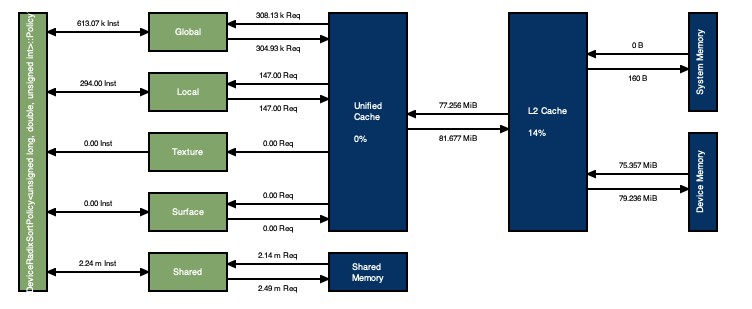
\includegraphics{attachments/louvain/Louvain_akamai.png}
\caption{Louvain\_akamai}
\end{figure}

It's clear that the bottleneck is at the device memory: most data are
read-once and write-once, with little possibility to reuse the data. The
kernel achieved 691 GB/s bandwidth utilization, \textasciitilde{}77\% of
the 32GB HBM2's 900 GB/s capability. This high-bandwidth utilization
fits the memory access pattern: mostly regular and coalesced.

The particular issue here is not the kernel implementation itself, it's
the usage of sorting: fully sorting the whole edge list is perhaps
overkill. One possible improvement is to use a custom hash table on the
GPU, to replace the sort + segmented reduce part. The hash table could
also cut the memory requirement by about 50\%.

\hypertarget{next-steps-4}{%
\section{Next Steps}\label{next-steps-4}}

\hypertarget{alternate-approaches-3}{%
\subsection{Alternate approaches}\label{alternate-approaches-3}}

\hypertarget{things-we-tried-that-didnt-work-well}{%
\subsubsection{Things we tried that didn't work
well}\label{things-we-tried-that-didnt-work-well}}

\textbf{Segmented sort and CUB segmented reduce}: the original idea for
modularity optimization is to use CUB's segmented sort and segmented
reduce within each vertex's neighborhood to get the vertex-community
weights. However, CUB uses one block per each segment in these two
routines, and that creates huge load imbalance, as the neighbor list
length can have large differences. The solution is 1) use
vertex-community pairs as keys, and CUB's unsegmented sort; 2) implement
a load-balanced segmented-reduce kernel. This solution reduces the
sort-reduce time by a few X, and can be enabled by the
\texttt{-\/-unify-segments} flag on the command line.

\textbf{STL hash table on CPU}: the \texttt{std::map} class has
performance issues when used in a multi-threading environment, and
yields poor scalability; it might be caused by using locks in the STL.
The solution is to use a size \(|V|\) array per thread for the vertices
that thread processes. Since within a thread, vertices are processed one
by one, and the maximum number of communities is \(|V|\), so instead of
a hash table, a flat size \(|V|\) array can replace the hash table. This
solution significantly reduces the running time, even using a single
thread. The multi-thread scalability is also much better.

\textbf{Vanilla hash table on GPU}: this can't be used, as keys
(vertex-community or community-community pair) and the values (edge
weights) are both 64-bit, and there is currently no support of
atomic-compare-and-exchange operations for 128-bit data. Even if that's
available, a vanilla table only provides insert and query operations,
but not accumulation of values for the same key.

\hypertarget{custom-hash-table}{%
\subsubsection{Custom hash table}\label{custom-hash-table}}

Hash tables can be used to accumulate the vertex-to-community weights
during modularity optimization iterations, and to get the
community-to-community edge weights during the graph contraction part of
the algorithm. Previous implementations use hash tables as a common
practice. However, as mentioned above, vanilla hash tables that store
key-value pairs are not a good choice for Louvain.

Louvain not only needs to store the key-value pairs, but also to
accumulate values associated with the same key. That key may be the same
vertex-community pair for modularity optimization, or the same
community-community pair for graph contraction. Ideally, if the hash
table provides the following functionality, it would be much more
suitable for Louvain:

\begin{itemize}
\tightlist
\item
  Only insert the key (in the first phase of using the hash table).
\item
  In the next phase, query the \emph{positions} of the keys, and use
  atomics to accumulate the values belonging to the same key, in a
  separate array.
\item
  There must be a barrier between the two phases; all insertions of the
  first phase need to be visible to the second phase.
\end{itemize}

This kind of hash table removes the strong restriction that the
key-value pair needs to be able to support an atomic
compare-and-exchange operation, which is imposed by vanilla hash table
implementations. The custom hash table is also more
value-accumulation-friendly. It replaces the sort-segmented reduce part,
and can reduce the workload from about \(O(6|E|)\) to \(O(2|E|)\), and
the memory requirement from \(48|E|\) bytes to \(24|E|\). However, the
memory access pattern now becomes irregular and uncoalesced, so it is
still unknown whether it can actually yield a performance gain.

\hypertarget{iteration-and-pass-stop-conditions}{%
\subsubsection{Iteration and pass stop
conditions}\label{iteration-and-pass-stop-conditions}}

The concurrent nature of the GPU implementation makes modularity gain
calculation inaccurate. Community migrations are also observed. Because
of these, the optimization iterations and the passes may run more than
needed, and resulted in longer running times, especially in the first
pass. Preliminary experiments to cap the number of iterations for the
first pass can reduce the running time by about 40\%, with the
modularity value roughly unchanged. The actual cap is dataset-dependent,
and more investigation is needed to get a better understanding of how to
set the cap.

\hypertarget{gunrock-implications-3}{%
\subsection{Gunrock implications}\label{gunrock-implications-3}}

The core of the Louvain implementation mainly uses all-edges advance,
sort, segmented reduce, and for loops. The sort-segmented reduce
operation is actually a segmented keyed reduce; if that's a common
operation that appears in more algorithms, it could be made into a new
operator. The all-edges advance is used quite often in several
applications, so wrapping it with a simpler operator interface could be
helpful.

\hypertarget{notes-on-multi-gpu-parallelization-4}{%
\subsection{Notes on multi-GPU
parallelization}\label{notes-on-multi-gpu-parallelization-4}}

When parallelizing across multiple GPUs, the community assignment of
local vertices and their neighbors needs to available locally, either
explicitly by moving them using communication functions, or implicitly
by peer memory access or unified virtual memory. The communication
volume is in the order of \(O(|V|)\) and the computation workload is at
least in \(O(|E|)\), so the scalability should be manageable.

When the number of GPUs is small, 1D partitioning can be used to divide
the edges, and replicate the vertices, so there is no need to do vertex
id conversion across multiple GPUs. When the number of GPUs is large,
the high-low degree vertex separation and partitioning scheme can be
used: edges are still distributed across GPUs, high degree vertices are
duplicated, and low degree vertices are owned by one GPU each. The
boundary to use different partitioning scheme is still unclear, but it's
likely that 8 GPUs within a DGX-1 can still be considered as a small
number, and use the simple 1D partitioning.

\hypertarget{notes-on-dynamic-graphs-4}{%
\subsection{Notes on dynamic graphs}\label{notes-on-dynamic-graphs-4}}

Louvain is not directly related to dynamic graphs. But it should be able
to run on a dynamic graph, provided the way to access all the edges is
the same. Community assignment from the previous graph can be used as a
good starting point, if the vertex ids are consistent and the graph is
not dramatically changed.

\hypertarget{notes-on-larger-datasets-4}{%
\subsection{Notes on larger datasets}\label{notes-on-larger-datasets-4}}

The bottleneck of memory usage of the current implementation is in the
edge pair-weight sort function: that makes up about half of the memory
usage. Replacing sort-segmented reduce with a custom hash table could
significantly lower the memory usage.

Louvain needs to go over the whole graph once in each modularity
optimization iteration. If the graph is larger than the combined GPU
memory space, which forces streaming of the graph in each modularity
optimization iteration, the performance bottleneck will be CPU-GPU
bandwidth. That can be an order of magnitude slower than when the graph
can fully fit in GPU memory. Considering the OpenMP implementation is
not that slow, using that may well be faster than moving the graph
multiple times across the CPU-GPU bridge.

\hypertarget{notes-on-other-pieces-of-this-workload-4}{%
\subsection{Notes on other pieces of this
workload}\label{notes-on-other-pieces-of-this-workload-4}}

All parts of Louvain are graph related, and fully implemented in
Gunrock.

\hypertarget{research-potential-2}{%
\subsection{Research potential}\label{research-potential-2}}

Community detection on graphs is generally an interesting research
topic, and others have targeted good GPU implementations for it. Our
work is the first time Louvain is mapped to sort and segmented reduce,
so more comparisons are needed to know whether it's better than the hash
table mapping. The custom hash table implementation is worth trying out,
and comparing with the current sort and segmented reduce implementation.
Multi-GPU implementations, particularly the graph contraction part, can
be a place for research investigation: it may be better to contract the
graph onto a single GPU, or even the CPU, when the graph is small; but
where is the threshold and how to do the multi-GPU to single-GPU or CPU
switch?

Label propagation is another algorithm for community detection. It has a
similar structure to Louvain, but has a simpler way to decide how to
move the vertices. Comparing them side by side for both result quality
(the modularity value) and computation speed (the running time) will be
beneficial.

\textbf{References}

{[}1{]} Hao Lu, Mahantesh Halappanavar, Ananth Kalyanaraman. ``Parallel
Heuristics for Scalable Community Detection'',
\url{https://arxiv.org/abs/1410.1237} (2015).

{[}2{]} Cheong C.Y., Huynh H.P., Lo D., Goh R.S.M. ``Hierarchical
Parallel Algorithm for Modularity-Based Community Detection Using
GPUs''. Euro-Par 2013.

{[}3{]} Md. Naim, Fredrik Manne, Mahantesh Halappanavar, and Antonio
Tumeo. ``Highly Scalable Community Detection Using a GPU'',
\url{https://www.eecs.wsu.edu/~assefaw/CSC16/abstracts/naim-CSC16_paper_14.pdf}
(2016).

{[}4{]} M. Naim, F. Manne, M. Halappanavar and A. Tumeo, ``Community
Detection on the GPU,'' IPDPS `17.

{[}5{]} Vincent D. Blondel, Jean-Loup Guillaume, Renaud Lambiotte,
Etienne Lefebvre, ``Fast unfolding of communities in large networks''.
\url{https://arxiv.org/abs/0803.0476} (2008).

\hypertarget{local-graph-clustering-lgc-1}{%
\chapter{Local Graph Clustering
(LGC)}\label{local-graph-clustering-lgc-1}}

From \href{https://projecteuclid.org/euclid.im/1243430567}{Andersen et
al.}:

\begin{quote}
A local graph partitioning algorithm finds a cut near a specified
starting vertex, with a running time that depends largely on the size of
the small side of the cut, rather than the size of the input graph.
\end{quote}

A common algorithm for local graph clustering is called PageRank-Nibble
(PRNibble), which solves the L1 regularized PageRank problem. We
implement a coordinate descent variant of this algorithm found in
\href{https://arxiv.org/pdf/1602.01886.pdf}{Fountoulakis et al.}, which
uses the fast iterative shrinkage-thresholding algorithm (FISTA).

\hypertarget{summary-of-results-5}{%
\section{Summary of Results}\label{summary-of-results-5}}

This variant of local graph clustering (L1 regularized PageRank via
FISTA) is a natural fit for Gunrock's frontier-based programming
paradigm. We observe speedups of 2-3 orders of magnitude over the HIVE
reference implementation.

The reference implementation of the algorithm was not explicitly written
as \texttt{advance}/\texttt{filter}/\texttt{compute} operations, but we
were able to quickly determine how to map the operations by using
\href{https://github.com/gunrock/pygunrock/blob/master/apps/pr_nibble.py}{a
lightweight Python implementation of the Gunrock programming API} as a
development environment. Thus, LGC was a good exercise in implementing a
non-trivial end-to-end application in Gunrock from scratch.

\hypertarget{summary-of-gunrock-implementation-4}{%
\section{Summary of Gunrock
Implementation}\label{summary-of-gunrock-implementation-4}}

We implement Algorithm 2 from
\href{https://arxiv.org/pdf/1602.01886.pdf}{Fountoulakis et al.}, which
maps nicely to Gunrock. We present the pseudocode below along with the
corresponding Gunrock operations:

\begin{verbatim}
A: adjacency matrix of graph
D: diagonal degree matrix of graph
Q: D^(-1/2) x (D - (1 - alpha)/2 x (D + A)) x D^(-1/2)
s: teleportation distribution, a distribution over nodes of graph
d_i: degree of node i
p_0: PageRank vector at iteration 0
q_0:  D^(-1/2) x p term that coordinate descent optimizes over
f(q): 1/2<q, Qq> - alpha x <s, D^(-1/2) x q>
grad_f_i(q_0): i'th term of the gradient of f(q_0) using q at iteration 0
rho: constant used to ensure convergence
alpha: teleportation constant in (0, 1)

Initialize: rho > 0
Initialize: q_0 = [0 ... 0]
Initialize: grad_f(q_0) = -alpha x D^(-1/2) x s

For k = 0, 1, ..., inf
    // Implemented using Gunrock ForAll operator
    Choose an i such that grad_f_i(q_k) < - alpha x rho x d_i^(1/2)
    q_k+1(i) = q_k(i) - grad_f_i(q_k)
    grad_f_i(q_k+1) = (1 - alpha)/2 x grad_f_i(q_k)

    // Implemented using Gunrock Advance and Filter operator
    For each j such that j ~ i
        Set grad_f_j(q_k+1) = grad_f_j(q_k) +
            (1 - alpha)/(2d_i^(1/2) x d_j^(1/2)) x A_ij x grad_f_i(q_k)

    For each j such that j !~ j
        Set grad_f_j(q_k+1) = grad_f_j(q_k)

    // Implemented using Gunrock ForEach operator
    // Note: ||y||_inf is the infinity norm
    if (||D^(-1/2) x grad_f(q_k)||_inf > rho x alpha)
            break
EndFor

return p_k = D^(1/2) x q_k
\end{verbatim}

\hypertarget{how-to-run-this-application-on-darpas-dgx-1-5}{%
\section{How To Run This Application on DARPA's
DGX-1}\label{how-to-run-this-application-on-darpas-dgx-1-5}}

\hypertarget{prereqsinput-4}{%
\subsection{Prereqs/input}\label{prereqsinput-4}}

\begin{Shaded}
\begin{Highlighting}[]
\CommentTok{# clone gunrock}
\FunctionTok{git}\NormalTok{ clone --recursive https://github.com/gunrock/gunrock.git \textbackslash{}}
\NormalTok{        -b dev-refactor}

\BuiltInTok{cd}\NormalTok{ gunrock/tests/pr_nibble}
\FunctionTok{cp}\NormalTok{ ../../gunrock/util/gitsha1.c.in ../../gunrock/util/gitsha1.c}
\FunctionTok{make}\NormalTok{ clean}
\FunctionTok{make}
\end{Highlighting}
\end{Shaded}

\hypertarget{running-the-application-5}{%
\subsection{Running the application}\label{running-the-application-5}}

\hypertarget{example-command-3}{%
\subsubsection{Example command}\label{example-command-3}}

\begin{Shaded}
\begin{Highlighting}[]
\ExtensionTok{./bin/test_pr_nibble_9.1_x86_64}\NormalTok{ \textbackslash{}}
\NormalTok{    --graph-type market \textbackslash{}}
\NormalTok{    --graph-file ../../dataset/small/chesapeake.mtx \textbackslash{}}
\NormalTok{    --src 0 \textbackslash{}}
\NormalTok{    --max-iter 1}
\end{Highlighting}
\end{Shaded}

\hypertarget{example-output-2}{%
\subsubsection{Example output}\label{example-output-2}}

\begin{verbatim}
Loading Matrix-market coordinate-formatted graph ...
  Reading meta data from ../../dataset/small/chesapeake.mtx.meta
  Reading edge lists from ../../dataset/small/chesapeake.mtx.coo_edge_pairs
  Substracting 1 from node Ids...
  Edge doubleing: 170 -> 340 edges
  graph loaded as COO in 0.084587s.
Converting 39 vertices, 340 directed edges ( ordered tuples) to CSR format...Done (0s).
Degree Histogram (39 vertices, 340 edges):
    Degree 0: 0 (0.000000 %)
    Degree 2^0: 0 (0.000000 %)
    Degree 2^1: 1 (2.564103 %)
    Degree 2^2: 22 (56.410256 %)
    Degree 2^3: 13 (33.333333 %)
    Degree 2^4: 2 (5.128205 %)
    Degree 2^5: 1 (2.564103 %)

__________________________
pr_nibble::CPU_Reference: reached max iterations. breaking at it=10
--------------------------
 Elapsed: 0.103951
==============================================
 advance-mode=LB
Using advance mode LB
Using filter mode CULL
__________________________
0    2   0   queue3      oversize :  234 ->  342
0    2   0   queue3      oversize :  234 ->  342
pr_nibble::Stop_Condition: reached max iterations. breaking at it=10
--------------------------
Run 0 elapsed: 1.738071, #iterations = 10
0 errors occurred.
[pr_nibble] finished.
 avg. elapsed: 1.738071 ms
 iterations: 140733299213840
 min. elapsed: 1.738071 ms
 max. elapsed: 1.738071 ms
 src: 0
 nodes_visited: 41513344
 edges_visited: 140733299212960
 nodes queued: 140733299212992
 edges queued: 5424992
 load time: 116.627 ms
 preprocess time: 963.004000 ms
 postprocess time: 0.080824 ms
 total time: 965.005875 ms
\end{verbatim}

\hypertarget{expected-output-2}{%
\subsection{Expected Output}\label{expected-output-2}}

We do not print the actual output values of PRNibble, but we output the
results of a correctness check of the GPU version against our CPU
implementation. \texttt{0\ errors\ occurred.} indicates that LGC has
generated an output that exactly matches our CPU validation
implementation.

Our implementations are validated against the
\href{https://gitlab.hiveprogram.com/ggillary/local_graph_clustering_socialmedia}{HIVE
reference implementation}.

For ease of exposition, and to help in mapping the workflow to Gunrock
primitives, we also implemented
\href{https://github.com/gunrock/pygunrock/blob/master/apps/pr_nibble.py}{a
version of PRNibble in pygunrock}. This implementation is nearly
identical to the actual Gunrock app, but in a way that more clearly
exposes the logic of the app and eliminates a lot of Gunrock
scaffolding/memory management/etc.

\hypertarget{performance-and-analysis-5}{%
\section{Performance and Analysis}\label{performance-and-analysis-5}}

Performance is measured by the runtime of the approximate PageRank
solver, given

\begin{itemize}
\tightlist
\item
  a graph \texttt{G=(U,\ E)}
\item
  a (set of) seed node(s) \texttt{S}
\item
  some parameters controlling e.g., the target conductivity of the
  output cluster (\texttt{rho}, \texttt{alpha}, \ldots{})
\end{itemize}

The reference implementation also includes a sweep-cut step, where a
threshold is applied to the approximate PageRank values to produce hard
cluster assignments. We do not implement this part of the workflow, as
it is not fundamentally a graph operation.

\hypertarget{implementation-limitations-5}{%
\subsection{Implementation
limitations}\label{implementation-limitations-5}}

PageRank runs on arbitrary graphs -- it does not require any special
conditions such as node attributes, etc.

\begin{itemize}
\item
  \textbf{Memory size}: The dataset is assumed to be an undirected graph
  (with no self-loops). We were able to run on graphs of up to 6.2 GB in
  size (7M vertices, 194M edges). The memory limitation should be the
  number of edges
  \texttt{2*\textbar{}E\textbar{}\ +\ 7*\textbar{}U\textbar{}}, which
  needs to be smaller than the GPU memory size (16 GB for a single P100
  on DGX-1).
\item
  \textbf{Data type}: We have only tested our implementations using an
  \texttt{int32} data type for node IDs. However, we could also support
  \texttt{int64} node IDs for graphs with more than 4B edges.
\end{itemize}

\hypertarget{comparison-against-existing-implementations-5}{%
\subsection{Comparison against existing
implementations}\label{comparison-against-existing-implementations-5}}

We compare our Gunrock GPU implementation with two CPU reference
implementations:

\begin{itemize}
\tightlist
\item
  \href{https://gitlab.hiveprogram.com/ggillary/local_graph_clustering_socialmedia}{HIVE
  reference implementation (Python wrapper around C++ library)}
\item
  \href{https://github.com/gunrock/gunrock/blob/dev-refactor/gunrock/app/pr_nibble/pr_nibble_test.cuh\#L38}{Gunrock
  CPU reference implementation (C++)}
\end{itemize}

We find the Gunrock implementation is 3 orders of magnitude faster than
either reference CPU implementation. The minimum, geometric mean, and
maximum speedups are 7.25x, 1297x, 32899x, respectively.

All runtimes are in milliseconds (ms):

\begin{longtable}[]{@{}lllll@{}}
\toprule
Dataset & HIVE Ref. C++ & Gunrock C++ & Gunrock GPU &
Speedup\tabularnewline
\midrule
\endhead
delaunay\_n13 & 21.52 & 16.33 & 2.86 & 8\tabularnewline
ak2010 & 97.99 & 72.08 & 3.04 & 32\tabularnewline
coAuthorsDBLP & 1004 & 1399 & 4.86 & 207\tabularnewline
belgium\_osm & 2270 & 1663 & 2.97 & 726\tabularnewline
roadNet-CA & 3403 & 2475 & 3.03 & 1123\tabularnewline
delaunay\_n21 & 5733 & 4084 & 2.98 & 1924\tabularnewline
cit-Patents & 40574 & 22148 & 16.41 & 2472\tabularnewline
hollywood-2009 & 43024 & 30430 & 46.30 & 929\tabularnewline
road\_usa & 48232 & 31617 & 3.01 & 16024\tabularnewline
delaunay\_n24 & 49299 & 34655 & 3.28 & 15030\tabularnewline
soc-LiveJournal1 & 63151 & 37936 & 19.29 & 3274\tabularnewline
europe\_osm & 97022 & 72973 & 2.95 & 32889\tabularnewline
indochina-2004 & 101877 & 71902 & 11.05 & 9220\tabularnewline
kron\_g500-logn21 & 110309 & 89438 & 627.55 & 176\tabularnewline
soc-orkut & 111391 & 89752 & 18.05 & 6171\tabularnewline
\bottomrule
\end{longtable}

\hypertarget{performance-limitations-5}{%
\subsection{Performance limitations}\label{performance-limitations-5}}

We profiled the Gunrock GPU primitives on the \texttt{kron\_g500-logn21}
graph. The profiler adds approx. 100 ms of overhead (728.48 ms with
profiler vs.~627.55 ms without profiler). The breakdown of runtime by
kernel looks like:

\begin{longtable}[]{@{}lll@{}}
\toprule
Gunrock Kernel & Runtime (ms) & Percentage of Runtime\tabularnewline
\midrule
\endhead
Advance (EdgeMap) & 566.76 & 77.8\%\tabularnewline
Filter (VertexMap) & 10.85 & 1.49\%\tabularnewline
ForAll (VertexMap) & 2.90 & 0.40\%\tabularnewline
Other & 147.89 & 20.3\%\tabularnewline
\bottomrule
\end{longtable}

\textbf{Note:} ``Other'' includes HtoD and DtoH memcpy, smaller kernels
such as scan, reduce, etc.

By profiling the LB Advance kernel, we find that the performance of
\texttt{advance} is bottlenecked by random memory accesses. In the first
part of the computation -- getting row pointers and column indices --
memory accesses can be coalesced and the profilers says we perform 4.9
memory transactions per access, which is close to the ideal of 4.
However, once we start processing these neighbors, the memory access
becomes random and we perform 31.2 memory transactions per access.

\hypertarget{next-steps-5}{%
\section{Next Steps}\label{next-steps-5}}

\hypertarget{alternate-approaches-4}{%
\subsection{Alternate approaches}\label{alternate-approaches-4}}

PRNibble can also be implemented in terms of matrix operations using our
GPU \href{https://github.com/owensgroup/GraphBLAS/}{GraphBLAS} library
-- this implementation is currently in progress.

In theory, local graph clustering is appealing because you don't have to
``touch'' the entire graph. However, all LGC implementations that we are
aware of first load the entire graph into CPU/GPU memory, which limits
the size of the graph that can be analyzed. Implementations that load
data from disk ``lazily'' as computation happens would be interesting
and practically useful.

\href{https://github.com/jshun/ligra}{Ligra} includes some high
performance implementations of similar algorithms. In the future, it
would be informative to benchmark our GPU implementation against those
performance optimized multi-threaded CPU implementations.

\hypertarget{gunrock-implications-4}{%
\subsection{Gunrock implications}\label{gunrock-implications-4}}

Gunrock currently supports all of the operations needed for this
application. In particular, the \texttt{ForAll} and \texttt{ForEach}
operators were very useful for this application.

Additionally, \texttt{pygunrock} proved to be a useful tool for
development -- correctly mapping the original (serial) algorithm to the
Gunrock operators required a lot of attention to detail, and having an
environment for rapid expedited experimentation facilitated the
algorithmic development.

\hypertarget{notes-on-multi-gpu-parallelization-5}{%
\subsection{Notes on multi-GPU
parallelization}\label{notes-on-multi-gpu-parallelization-5}}

Since this problem maps well to Gunrock operations, we expect
parallelization strategy would be similar to BFS and SSSP. The dataset
can be effectively divided across multiple GPUs.

\hypertarget{notes-on-dynamic-graphs-5}{%
\subsection{Notes on dynamic graphs}\label{notes-on-dynamic-graphs-5}}

It is not obvious how this algorithm would be extended to handle dynamic
graphs. At a high level, the algorithm iteratively spreads mass from the
seed nodes to neighbors in the graph. As the connectivity structure of
the graph changes, the dynamics of this mass spreading could change
arbitrarily -- imagine edges that form bridges between two previously
distinct clusters. Thus, we suspect that adapting the app to work on
dynamic graphs may require substantial development and study of the
underlying algorithms.

\hypertarget{notes-on-larger-datasets-5}{%
\subsection{Notes on larger datasets}\label{notes-on-larger-datasets-5}}

If the data were too big to fit into the aggregate GPU memory of
multiple GPUs on a single node, then we would need to look at
multiple-node solutions. Getting the application to work on multiple
nodes would not be challenging, because it is very similar to BFS.
However, optimizing it to achieve good scalability may require
asynchronous communication, an area where we have some experience
(\href{https://arxiv.org/pdf/1803.03922.pdf}{Pan et al.}). Asynchronous
communication may be necessary in order to reach better scalability in
multi-node, because this application which can be formulated as
sparse-matrix vector multiplication has limited computational intensity
(low computation-to-communication).

\hypertarget{notes-on-other-pieces-of-this-workload-5}{%
\subsection{Notes on other pieces of this
workload}\label{notes-on-other-pieces-of-this-workload-5}}

As mentioned previously, we do not implement the sweep-cut portion of
the workflow where the PageRank values are discretized to produce hard
cluster assignments. Though it's not fundamentally a graph problem,
parallelization of this step is a research question addressed in
\href{https://arxiv.org/abs/1604.07515}{Shun et al}.

\hypertarget{potential-future-academic-work}{%
\subsection{Potential future academic
work}\label{potential-future-academic-work}}

The coordinate descent implementation (developed by Ben Johnson) shows
that Gunrock can be used as a coordinate descent solver. There has been
more interest in coordinate descent recently, because coordinate descent
can be used in ML as an alternative to stochastic gradient descent for
SVM training.

\hypertarget{references}{%
\subparagraph{References}\label{references}}

Prof.~Cho-Jui Hsieh from UC Davis is an expert in this field (see
\href{http://www.jmlr.org/proceedings/papers/v37/hsieha15-supp.pdf}{1},
\href{https://www.semanticscholar.org/paper/HogWild\%2B\%2B\%3A-A-New-Mechanism-for-Decentralized-Zhang-Hsieh/183d421bfb807378bd0463894415f40e0fca64d6}{2},
\href{http://www.stat.ucdavis.edu/~chohsieh/passcode_fix.pdf}{3}).

\hypertarget{graph-projections-1}{%
\chapter{Graph Projections}\label{graph-projections-1}}

Given a (directed) graph \texttt{G}, graph projection outputs a graph
\texttt{H} such that \texttt{H} contains edge \texttt{(u,\ v)} iff
\texttt{G} contains edges \texttt{(w,\ u)} and \texttt{(w,\ v)} for some
node \texttt{w}. That is, graph projection creates a new graph where
nodes are connected iff they are neighbors of the same node in the
original graph. Typically, the edge weights of \texttt{H} are computed
via some (simple) function of the corresponding edge weights of
\texttt{G}.

Graph projection is most commonly used when the input graph \texttt{G}
is bipartitite with node sets \texttt{U1} and \texttt{U2} and directed
edges \texttt{(u,\ v)}. In this case, the operation yields a unipartite
projection onto one of the node sets. However, graph projection can also
be applied to arbitrary (unipartite) graphs.

\hypertarget{summary-of-results-6}{%
\section{Summary of Results}\label{summary-of-results-6}}

Because it has a natural representation in terms of sparse matrix
operations, graph projections gave us an opportunity to compare ease of
implementation and performance between Gunrock and another UC-Davis
project, GPU \href{https://github.com/owensgroup/GraphBLAS}{GraphBLAS}.

Overall, we found that Gunrock was more flexible and more performant
than GraphBLAS, likely due to better load balancing. However, in this
case, the GraphBLAS application was substantially easier to program than
Gunrock, and also allowed us to take advantage of some more
sophisticated memory allocation methods available in the GraphBLAS
cuSPARSE backend. These findings suggest that addition of certain
commonly used API functions to Gunrock could be a fruitful direction for
further work.

\hypertarget{summary-of-gunrock-implementation-5}{%
\section{Summary of Gunrock
Implementation}\label{summary-of-gunrock-implementation-5}}

We implement two versions of graph projections: one using
\href{https://github.com/gunrock/gunrock}{Gunrock} and one using
\href{https://github.com/owensgroup/GraphBLAS}{GraphBLAS}.

\hypertarget{gunrock}{%
\subsubsection{Gunrock}\label{gunrock}}

First, we can compute graph projection in Gunrock via a single
\texttt{advance} operation from all nodes w/ nonzero outgoing degree:

\begin{verbatim}
def _advance_op(self, G, H_edges, src, dest):
    for neib in G.neighbors(src):
        if dest != neib:
            H_edges[dest * G.num_nodes + neib] += 1
\end{verbatim}

That is, for each edge in the graph, we fetch the neighbors of the
source node in \texttt{G}, then increment the weight of the edge between
\texttt{dest} and each of those neighbors in \texttt{H\_edges}.

Note that we have only implemented the unweighted case and a single
method for computing the edgeweights of \texttt{H}, but the extension to
weighted graphs and different weighting functions would be
straightforward.

We use a dense \texttt{\textbar{}V\textbar{}x\textbar{}V\textbar{}}
array to store the edges of the output matrix \texttt{H}. This is simple
and fast, but uses an unreasonably large amount of memory (a graph with
60k nodes requires 16 GB). In the worst-case scenario, \texttt{H} may
actually have all \texttt{\textbar{}V\textbar{}x\textbar{}V\textbar{}}
possible edges, but any typical real-world graph has \emph{far} fewer
edges in practice.

\hypertarget{graphblas}{%
\subsubsection{GraphBLAS}\label{graphblas}}

Second, we implement graph projection as a single sparse matrix-matrix
multiply in our
\href{https://github.com/owensgroup/GraphBLAS}{GraphBLAS} GPU library,
which wraps and extends cuSPARSE.

Graph projection admits a simple linear algebra formulation. Given the
adjacency matrix \texttt{A} of graph \texttt{G}, the projection is just:

\begin{verbatim}
H = matmul(transpose(A), A)
\end{verbatim}

which can be concisely implemented via cuSPARSE's \texttt{csr2csc} and
\texttt{csrgemm} functions.

The \texttt{csrgemm} functions in cuSPARSE allocate memory more
intelligently than we do above, on the order of the number of edges in
the output. Thus, our GraphBLAS implementation can scale to
substantially larger matrices than our Gunrock implementation. However,
implementing graph projection via a single call to \texttt{csrgemm}
requires both the input graph \texttt{G} and output graph \texttt{H} to
fit in GPU memory (16 GB on the DGX-1). This limit can easily be hit,
even for a moderately sized \texttt{G}, as the number of edges in
\texttt{H} is often orders of magnitude larger than in \texttt{G}.

Thus, to scale to larger graphs, we implement graph projections via a
chunked matrix multiply. Specifically, to compute \texttt{matmul(X,\ Y)}
w/ \texttt{X.shape\ =\ (n,\ m)} and \texttt{Y.shape\ =\ (m,\ k)}, we
split \texttt{X} into \texttt{c} matrices \texttt{(X\_1,\ ...,\ X\_c)},
w/ \texttt{X\_i.shape\ =\ (n\ /\ c,\ m)}. Then we compute
\texttt{matmul(X\_i,\ Y)} for each \texttt{X\_i}, moving the output of
each multiplication from GPU to CPU memory as we go. This implementation
addresses the common case where we can fit both \texttt{X} and
\texttt{Y} in GPU memory, but not \texttt{matmul(X,\ Y)}. Obviously, the
chunked matrix multiply incurs a performance penalty, but allows us to
run graph projections of much larger graphs on the GPU.

\hypertarget{how-to-run-this-application-on-darpas-dgx-1-6}{%
\section{How To Run This Application on DARPA's
DGX-1}\label{how-to-run-this-application-on-darpas-dgx-1-6}}

\hypertarget{gunrock-1}{%
\subsection{Gunrock}\label{gunrock-1}}

\hypertarget{prereqsinput-5}{%
\subsubsection{Prereqs/input}\label{prereqsinput-5}}

\begin{Shaded}
\begin{Highlighting}[]
\FunctionTok{git}\NormalTok{ clone --recursive https://github.com/gunrock/gunrock -b dev-refactor}
\BuiltInTok{cd}\NormalTok{ gunrock/tests/proj/}
\FunctionTok{cp}\NormalTok{ ../../gunrock/util/gitsha1.c.in ../../gunrock/util/gitsha1.c}
\FunctionTok{make}\NormalTok{ clean}
\FunctionTok{make}
\end{Highlighting}
\end{Shaded}

\hypertarget{application-specific-parameters-2}{%
\subsubsection{Application specific
parameters}\label{application-specific-parameters-2}}

None

\hypertarget{example-command-4}{%
\subsubsection{Example Command}\label{example-command-4}}

\begin{Shaded}
\begin{Highlighting}[]
\ExtensionTok{./bin/test_proj_9.1_x86_64}\NormalTok{ \textbackslash{}}
\NormalTok{        --graph-type market \textbackslash{}}
\NormalTok{        --graph-file ../../dataset/small/chesapeake.mtx}
\end{Highlighting}
\end{Shaded}

\hypertarget{example-output-3}{%
\subsubsection{Example Output}\label{example-output-3}}

\begin{verbatim}
Loading Matrix-market coordinate-formatted graph ...
Reading from ../../dataset/small/chesapeake.mtx:
  Parsing MARKET COO format edge-value-seed = 1539110067
 (39 nodes, 340 directed edges)...
Done parsing (0 s).
  Converting 39 vertices, 340 directed edges ( ordered tuples) to CSR format...
Done converting (0s).
__________________________
--------------------------
 Elapsed: 0.026941
Using advance mode LB
Using filter mode CULL
__________________________
0    0   0   queue3      oversize :  234 ->  342
0    0   0   queue3      oversize :  234 ->  342
--------------------------
Run 0 elapsed: 0.199080, #iterations = 1
edge_counter=1372
0->1 | GPU=9.000000 CPU=9.000000
0->2 | GPU=1.000000 CPU=1.000000
0->3 | GPU=2.000000 CPU=2.000000
...
38->35 | GPU=28.000000 CPU=28.000000
38->36 | GPU=2.000000 CPU=2.000000
38->37 | GPU=18.000000 CPU=18.000000
======= PASSED ======
[proj] finished.
 avg. elapsed: 0.199080 ms
 iterations: 38594739
 min. elapsed: 0.199080 ms
 max. elapsed: 0.199080 ms
 src: 0
 nodes_visited: 38578864
 edges_visited: 38578832
 nodes queued: 140734466796512
 edges queued: 140734466795232
 load time: 85.5711 ms
 preprocess time: 955.861000 ms
 postprocess time: 3.808022 ms
 total time: 960.005045 ms
\end{verbatim}

\hypertarget{expected-output-3}{%
\subsubsection{Expected Output}\label{expected-output-3}}

When run in \texttt{verbose} mode, the app outputs the weighted edgelist
of the graph projection \texttt{H}. When run in \texttt{quiet} mode, it
only outputs performance statistics and the results of a correctness
check.

\hypertarget{graphblas-1}{%
\subsection{GraphBLAS}\label{graphblas-1}}

\hypertarget{prereqsinput-6}{%
\subsubsection{Prereqs/input}\label{prereqsinput-6}}

\begin{Shaded}
\begin{Highlighting}[]
\FunctionTok{git}\NormalTok{ clone --recursive https://github.com/bkj/graphblas_proj}
\BuiltInTok{cd}\NormalTok{ graphblas_proj}
\FunctionTok{make}\NormalTok{ clean}
\FunctionTok{make}
\end{Highlighting}
\end{Shaded}

\hypertarget{application-specific-parameters-3}{%
\subsubsection{Application specific
parameters}\label{application-specific-parameters-3}}

\begin{verbatim}
--unweighted
 1 = convert entries of adjacency matrix to 1
 0 = leave entries of adjacency matrix as-is
--proj-debug
 1 = print debug information
 0 = don't print debug information
--print-results
 1 = print the edges of the projected graph
 0 = don't print edges
--onto-cols
 1 = given adjacency matrix A w/ `A.shape = (m, n)`,
     compute projection `H = matmul(transpose(A), A)` w/ `H.shape = (n, n)`
 0 = given adjacency matrix A w/ `A.shape = (m, n)`,
     compute projection `H = matmul(A, transpose(A))` w/ `H.shape = (m, m)`
--num-chunks
 <= 1 = do matrix multiply in one step
  > 1 = break matrix multiply into multiple chunks (eg, so we can compute
        projections larger than GPU memory)
\end{verbatim}

\hypertarget{example-command-5}{%
\subsubsection{Example Command}\label{example-command-5}}

\begin{Shaded}
\begin{Highlighting}[]
\CommentTok{# generate some random data `data/X.mtx`}
\ExtensionTok{python}\NormalTok{ data/make-random.py --seed 111 \textbackslash{}}
\NormalTok{        --num-rows 1000 --num-cols 1000 --density 0.1}

\CommentTok{# run graph projection}
\ExtensionTok{./proj}\NormalTok{ --X data/X.mtx --unweighted 1 --proj-debug 1}
\end{Highlighting}
\end{Shaded}

\hypertarget{example-output-4}{%
\subsubsection{Example Output}\label{example-output-4}}

\begin{verbatim}
proj.cu: loading data/X.mtx
  done
proj.cu: computing transpose
  done
proj.cu: computing projection
mxm analyze successful!
mxm compute successful!
  done
proj_num_edges          = 999946  # number of edges in H, including self loops
dim_out                 = 1000    # dimension of projected graph
proj_num_edges (noloop) = 998946  # number of edges in H, excluding self loops
timer                   = 208.98  # elapsed time (no IO)
\end{verbatim}

\hypertarget{expected-output-4}{%
\subsubsection{Expected Output}\label{expected-output-4}}

The app will print the number of edges in the projected graph.
Additionally,

\begin{itemize}
\tightlist
\item
  When run w/ \texttt{-\/-print-results=1}, the app prints the edges of
  the the graph projection \texttt{H}.
\item
  When run w/ \texttt{-\/-proj-debug=1}, the app prints a small number
  of progress messages.
\end{itemize}

\hypertarget{validation-1}{%
\section{Validation}\label{validation-1}}

We compared the results of the Gunrock implementation to the
\href{https://hiveprogram.com/wiki/display/WOR/V0+-+Application+Classification}{HIVE
reference implementation} and the
\href{https://gitlab.hiveprogram.com/jfiroz/graph_projection}{PNNL
implementation}. These two implementations vary slightly in their output
(e.g., handling of self loops). We validated the correctness of our
results against the HIVE reference implementation.

\hypertarget{performance-and-analysis-6}{%
\section{Performance and Analysis}\label{performance-and-analysis-6}}

Performance is measured by the runtime of the app, given:

\begin{itemize}
\tightlist
\item
  an input graph \texttt{G} (possibly bipartite)
\item
  whether to project onto the rows or columns of the graph.
\end{itemize}

\hypertarget{implementation-limitations-6}{%
\subsection{Implementation
limitations}\label{implementation-limitations-6}}

\hypertarget{gunrock-2}{%
\subsubsection{Gunrock}\label{gunrock-2}}

The primary limitation of the current implementation is that it
allocates a \texttt{\textbar{}V\textbar{}x\textbar{}V\textbar{}} array,
where \texttt{\textbar{}V\textbar{}} is the number of nodes in the
network. This means that the memory requirements of the app can easily
exceed the memory available on a single GPU (16 GB on the DGX-1). The
size of this array reflects the \emph{worst case} memory requirements of
the graph projection workflow; while some graphs can become
exceptionally large and dense when projected, we should be able to run
the app on larger graphs if we store the output in a different data
structure and/or allocate memory more efficiently. Algorithms do exist
for mitigating this issue: cuSPARSE's \texttt{csrgemm} method computes
the row pointers in one pass, then allocates the exact amount of memory
for \texttt{H}'s column and value arrays, then actually computes the
matrix product. An interesting future direction would be to integrate
this sort of algorithm into Gunrock.

It may be possible to improve performance by making assumptions about
the topology of the graph. Graph projection is often used for bipartite
graphs, but this app does not make any assumptions about the topology of
the graph. This choice was made in order to remain consistent with the
\href{https://hiveprogram.com/wiki/display/WOR/V0+-+Application+Classification}{HIVE
reference implementation}.

There are various ways that the edges of the output graph \texttt{H} can
be weighted. We only implement graph projections for unweighted graphs:
the weight of the edge \texttt{(u,\ v)} in the output graph \texttt{H}
is the count of (incoming) neighbors that \texttt{u} and \texttt{v} have
in common in the original graph \texttt{G}. Implementation of other
weight functions would be fairly straightforward.

\hypertarget{graphblas-2}{%
\subsubsection{GraphBLAS}\label{graphblas-2}}

Currently, for the chunked matrix multiply, the CPU memory allocation
and GPU to CPU memory copies for \texttt{matmul(X\_i,\ Y)} block the
computation of \texttt{matmul(X\_{[}i+1{]},\ Y)}. We could implement
this in a non-blocking way using CUDA streams, but this would require
some redesign of the GraphBLAS APIs.

Certain weighting functions are easily implemented by applying a
transformation to the values of the sparse adjacency matrix \texttt{A},
but others cannot. For instance, these weighting functions are easy to
implement:

\begin{verbatim}
    weight_out = 1                             (by setting both matrices entries to 1)
    weight_out = weight_edge_1                 (by setting one matrix's entries to 1)
    weight_out = weight_edge_1 / weight_edge_2 (by setting one matrix's entries to 1 / x)
    ...
\end{verbatim}

while this function (from the HIVE reference implementation) is not easy
to implement in the \texttt{cuSPARSE} plus/multiply semiring:

\begin{verbatim}
        weight_out = weight_edge_1 / (weight_edge_1 + weight_edge_2)
\end{verbatim}

Implementation of additional semirings in GraphBLAS is currently in
progress, and will extend the family of weightings we could support.

\hypertarget{comparison-against-existing-implementations-6}{%
\subsection{Comparison against existing
implementations}\label{comparison-against-existing-implementations-6}}

When the graph fits in its memory, the Gunrock implementation is approx.
5x faster than the GraphBLAS implementation and approx. 100x faster than
PNNL's OpenMP CPU implemention w/ 64 threads. Somewhat surprisingly,
PNNL's implementation is substantially slower than a single-threaded
scipy sparse matrix multiplication.

When the graph does not fit in the Gunrock implementation's memory, our
GPU GraphBLAS implementation is the fastest of the remaining
implementations.

\hypertarget{existing-implementations}{%
\subsubsection{Existing
implementations}\label{existing-implementations}}

\hypertarget{pnnl}{%
\paragraph{PNNL}\label{pnnl}}

We compare our results against
\href{https://gitlab.hiveprogram.com/jfiroz/graph_projection}{PNNL's
OpenMP reference implementation}. We make
\href{https://gitlab.hiveprogram.com/bjohnson/graph_projection/commit/b37aabe2e56fe5207bc22c09c029b7e88c0327c1}{minor
modifications} to their code to handle unweighted graphs, in order to
match the Gunrock and GraphBLAS implementations. That is, the weight of
the edge in the output graph \texttt{H} is the number of shared
neighbors in the original graph.

There is a \texttt{-\/-simple} flag in PNNL's CLI, but examining the
code reveals that it just changes the order of operations. Thus, all of
our experiments are conducted with \texttt{-\/-simple=1}, which is
faster than \texttt{-\/-simple=0} due to better data access patterns.

\hypertarget{scipy}{%
\paragraph{Scipy}\label{scipy}}

A very simple baseline is sparse matrix-matrix multiplication as
implemented in the popular \texttt{scipy} python package. This is a
single-threaded C++ implementation with a Python wrapper. Note, this
implementation comes with the same caveats about weighting functions as
the Gunrock implementation.

\hypertarget{experiments}{%
\subsubsection{Experiments}\label{experiments}}

\hypertarget{movielens}{%
\paragraph{MovieLens}\label{movielens}}

MovieLens is a bipartite graph \texttt{G=(U,\ V,\ E)} w/
\texttt{\textbar{}U\textbar{}=138493},
\texttt{\textbar{}V\textbar{}=26744} and
\texttt{\textbar{}E\textbar{}=20000264}. We report results on the full
graph, as well as several random subgraphs.

For PNNL's OpenMP implementation, we report results using \{1, 2, 4, 8,
16, 32, 64\} threads.

In all cases, we project onto the nodeset
\texttt{\textbar{}V\textbar{}}, producing a
\texttt{\textbar{}V\textbar{}x\textbar{}V\textbar{}} graph.

\textbf{Note:} Small differences in the number of nonzero entries in the
output (nnz\_out) are due to small book-keeping differences
(specifically, keeping or dropping self-loops). These differences do not
have any meaningful impact on runtimes.

\hypertarget{m-edge-subgraph-u6743-v13950-e1m}{%
\subparagraph{1M edge subgraph (\textbar{}U\textbar{}=6743
\textbar{}V\textbar{}=13950
\textbar{}E\textbar{}=1M)}\label{m-edge-subgraph-u6743-v13950-e1m}}

\begin{longtable}[]{@{}llll@{}}
\toprule
implementation & num\_threads & nnz\_out &
elapsed\_seconds\tabularnewline
\midrule
\endhead
scipy & 1 & 63104132 & 2.4912\tabularnewline
PNNL OpenMP & 1 & 63090182 & 61.4852\tabularnewline
PNNL OpenMP & 2 & 63090182 & 62.2842\tabularnewline
PNNL OpenMP & 4 & 63090182 & 60.1542\tabularnewline
PNNL OpenMP & 8 & 63090182 & 37.5853\tabularnewline
PNNL OpenMP & 16 & 63090182 & 22.0257\tabularnewline
PNNL OpenMP & 32 & 63090182 & 13.1482\tabularnewline
PNNL OpenMP & 64 & 63090182 & 9.055\tabularnewline
Gunrock & 1xP100 GPU & 63090182 & \textbf{0.060}\tabularnewline
GraphBLAS & 1xP100 GPU & 63090182 & 0.366\tabularnewline
\bottomrule
\end{longtable}

\hypertarget{m-edge-subgraph-u34395-v20402-e5m}{%
\subparagraph{5M edge subgraph (\textbar{}U\textbar{}=34395
\textbar{}V\textbar{}=20402
\textbar{}E\textbar{}=5M)}\label{m-edge-subgraph-u34395-v20402-e5m}}

\begin{longtable}[]{@{}llll@{}}
\toprule
implementation & num\_threads & nnz\_out &
elapsed\_seconds\tabularnewline
\midrule
\endhead
scipy & 1 & 157071858 & 10.1052\tabularnewline
PNNL OpenMP & 1 & 157051456 & 357.511\tabularnewline
PNNL OpenMP & 2 & 157051456 & 309.723\tabularnewline
PNNL OpenMP & 4 & 157051456 & 218.519\tabularnewline
PNNL OpenMP & 8 & 157051456 & 113.987\tabularnewline
PNNL OpenMP & 16 & 157051456 & 57.4606\tabularnewline
PNNL OpenMP & 32 & 157051456 & 38.1186\tabularnewline
PNNL OpenMP & 64 & 157051456 & 29.0056\tabularnewline
Gunrock & 1xP100 GPU & 157051456 & \textbf{0.3349}\tabularnewline
GraphBLAS & 1xP100 GPU & 157051456 & 1.221\tabularnewline
\bottomrule
\end{longtable}

\hypertarget{movielens-20m-graph-u138493-v26744-e20m}{%
\subparagraph{MovieLens-20M graph (\textbar{}U\textbar{}=138493
\textbar{}V\textbar{}=26744
\textbar{}E\textbar{}=20M)}\label{movielens-20m-graph-u138493-v26744-e20m}}

\begin{longtable}[]{@{}llll@{}}
\toprule
implementation & num\_threads & nnz\_out &
elapsed\_seconds\tabularnewline
\midrule
\endhead
scipy & 1 & 286857534 & 39.181\tabularnewline
PNNL OpenMP & 1 & 286830790 & \emph{I killed before
finish}\tabularnewline
PNNL OpenMP & 2 & 286830790 & 1109.32\tabularnewline
PNNL OpenMP & 4 & 286830790 & 727.224\tabularnewline
PNNL OpenMP & 8 & 286830790 & 358.708\tabularnewline
PNNL OpenMP & 16 & 286830790 & 188.701\tabularnewline
PNNL OpenMP & 32 & 286830790 & 102.964\tabularnewline
PNNL OpenMP & 64 & 286830790 & 163.731\tabularnewline
Gunrock & 1xP100 GPU & 286830790 & \emph{out-of-memory}\tabularnewline
GraphBLAS & 1xP100 GPU & 286830790 & \textbf{5.012}\tabularnewline
\bottomrule
\end{longtable}

\textbf{Takeaway:} When the graph is small enough, Gunrock graph
projection is fastest, followed by GraphBLAS (approx. 5x slower). The
PNNL OpenMP implementation is consistently substantially slower than the
single threaded scipy implementation, even when using 32+ threads.

\hypertarget{rmat}{%
\paragraph{RMAT}\label{rmat}}

Next we test on a
\href{https://graphchallenge.s3.amazonaws.com/synthetic/graph500-scale18-ef16/graph500-scale18-ef16_adj.tsv.gz}{scale
18 RMAT graph}. This is \emph{not} a bipartite graph, but the graph
projection algorithm can still be applied.

This graph was chosen because it was used in benchmarks in
\href{https://gitlab.hiveprogram.com/jfiroz/graph_projection}{PNNL's
gitlab repo}. However, their command line parameters appear to be
incorrect, so our results here are substantially different than reported
in their README.

\hypertarget{rmat-18-v174147-e7600696}{%
\subparagraph{RMAT-18 (\textbar{}V\textbar{}=174147
\textbar{}E\textbar{}=7600696)}\label{rmat-18-v174147-e7600696}}

\begin{longtable}[]{@{}llll@{}}
\toprule
implementation & num\_threads & nnz\_out &
elapsed\_seconds\tabularnewline
\midrule
\endhead
scipy & 1 & 2973926895 & 150.869\tabularnewline
PNNL OpenMP & 1 & 2973752748 & \emph{I killed before
finish}\tabularnewline
PNNL OpenMP & 2 & 2973752748 & \emph{I killed before
finish}\tabularnewline
PNNL OpenMP & 4 & 2973752748 & 812.453\tabularnewline
PNNL OpenMP & 8 & 2973752748 & 677.582\tabularnewline
PNNL OpenMP & 16 & 2973752748 & 419.468\tabularnewline
PNNL OpenMP & 32 & 2973752748 & 369.278\tabularnewline
PNNL OpenMP & 64 & 2973752748 & 602.69\tabularnewline
Gunrock & 1xP100 GPU & 2973752748 & \emph{out-of-memory}\tabularnewline
GraphBLAS & 1xP100 GPU & 2973752748 & \textbf{26.478}\tabularnewline
\bottomrule
\end{longtable}

\textbf{Takeaway:} GraphBLAS is approx. 5.7x faster than scipy, the next
fastest implementation. Again, the PNNL OpenMP implementation is
substantially faster than the single-threaded scipy implementation.

\emph{When the dataset can fit into memory}, Gunrock is
\textasciitilde{} 4x faster than GraphBLAS. Since the two
implementations use slightly different algorithms, it's hard to tell
where the Gunrock speedup comes from. Our hunch is that Gunrock's
superior load balancing gives better performance than GraphBLAS, but
this is an interesting topic for further research.

\hypertarget{performance-information}{%
\subsection{Performance information}\label{performance-information}}

\hypertarget{gunrock-3}{%
\subsubsection{Gunrock}\label{gunrock-3}}

\begin{itemize}
\tightlist
\item
  Results of profiling indicate that the Gunrock implementation is bound
  by memory latency.
\item
  The device memory bandwidth is 297 GB/s -- within the expected range
  for Gunrock graph analytics.
\item
  92\% of the runtime is spent in the advance operator (pseudocode in
  implementation summary)
\end{itemize}

\hypertarget{graphblas-3}{%
\subsubsection{GraphBLAS}\label{graphblas-3}}

\begin{itemize}
\tightlist
\item
  99\% of time is spent in cuSPARSE's \texttt{csrgemm} routines
\end{itemize}

\hypertarget{next-steps-6}{%
\section{Next Steps}\label{next-steps-6}}

\hypertarget{alternate-approaches-5}{%
\subsection{Alternate approaches}\label{alternate-approaches-5}}

As mentioned above, it would be worthwhile to implement a Gunrock
version that does not require allocating the
\texttt{\textbar{}V\textbar{}x\textbar{}V\textbar{}} array. It should be
possible to achieve this by implementing the same kind of two-pass
approach that cuSPARSE uses for \texttt{spgemm} -- one pass computes the
CSR offsets, then column and data values are inserted at the appropriate
locations.

\hypertarget{gunrock-implications-5}{%
\subsection{Gunrock implications}\label{gunrock-implications-5}}

Gunrock does not natively support bipartite graphs, but it is
straightforward for programmers to implement algorithms that expect
bipartite graphs by keeping track of the number of nodes in each node
set. However, for multi-GPU implementations, the fact that a graph is
bipartite may be useful for determining the optimal graph partitioning.

\hypertarget{notes-on-multi-gpu-parallelization-6}{%
\subsection{Notes on multi-GPU
parallelization}\label{notes-on-multi-gpu-parallelization-6}}

Multiple GPU support for GraphBLAS is on the roadmap. Unlike the Seeded
Graph Matching problem -- which requires the \texttt{mxm}, \texttt{mxv}
and \texttt{vxm} primitives, which in turn necessitates possible changes
in data layout -- this problem only requires the \texttt{mxm} primitive,
so multiple GPU support for graph projections is easier than for SGM.

Even though extending matrix multiplication to multiple GPUs can be
straightforward, doing so in a backend-agnostic fashion that abstracts
away the placement (i.e.~which part of matrix A goes on which GPU) may
still be quite challenging.

Further discussion can be found
\href{https://gunrock.github.io/docs/hive_year1_summary.html\#scaling-analysis-for-hive-applications}{here}.

\hypertarget{notes-on-dynamic-graphs-6}{%
\subsection{Notes on dynamic graphs}\label{notes-on-dynamic-graphs-6}}

This workflow does not have an explicit dynamic component. The graph
projection operation seems like it would be fairly straightforward to
adapt to dynamic graphs -- as nodes/edges are added to \texttt{G}, we
create/increment the weight of the appropriate edges in \texttt{H}.
However, this adds an additional layer of complexity to the memory
allocation step, as we can't use the two-pass approach to allocate
memory conservatively.

\hypertarget{notes-on-larger-datasets-6}{%
\subsection{Notes on larger datasets}\label{notes-on-larger-datasets-6}}

If the dataset were too big to fit into the aggregate GPU memory of
multiple GPUs on a node, then two directions can be taken in order to be
able to tackle these larger datasets:

\begin{itemize}
\tightlist
\item
  Out-of-memory: Compute using part of the dataset at a time on the GPU,
  and save the completed result to CPU memory. This method is slower
  than distributed, but cheaper and easier to implement.
\item
  Distributed memory: If GPU memory of a single node is not enough, use
  multiple nodes. This method can be made to scale for infinitely large
  datasets provided the implementation is good enough (faster than
  out-of-memory, but more expensive and difficult).
\end{itemize}

\hypertarget{notes-on-other-pieces-of-this-workload-6}{%
\subsection{Notes on other pieces of this
workload}\label{notes-on-other-pieces-of-this-workload-6}}

This workload does not involve any non-graph components.

\hypertarget{seeded-graph-matching-sgm-1}{%
\chapter{Seeded Graph Matching
(SGM)}\label{seeded-graph-matching-sgm-1}}

From \href{https://arxiv.org/pdf/1209.0367.pdf}{Fishkind et al.}:

\begin{verbatim}
Given two graphs, the graph matching problem is to align the two vertex sets
so as to minimize the number of adjacency disagreements between the two graphs.
The seeded graph matching problem is the graph matching problem when we are
first given a partial alignment that we are tasked with completing.
\end{verbatim}

That is, given two graphs \texttt{A} and \texttt{B}, we seek to find the
permutation matrix \texttt{P} that maximizes the number of adjacency
agreements between \texttt{A} and \texttt{P\ *\ B\ *\ P.T}, where
\texttt{*} represents matrix multiplication. The algorithm Fishkind et
al.~propose first relaxes the hard 0-1 constraints on \texttt{P} to the
set of doubly stochastic matrices (each row and column sums to 1), then
uses the Frank-Wolfe algorithm to minimize the objective function
\texttt{sum((A\ -\ P\ *\ B\ *\ P.T)\ **\ 2)}. Finally, the relaxed
solution is projected back onto the set of permutation matrices to yield
a feasible solution.

\hypertarget{summary-of-results-7}{%
\section{Summary of Results}\label{summary-of-results-7}}

SGM is a fruitful workflow to optimize, because the existing
implementations were not written with performance in mind. By making
minor modifications to the algorithm that allow use of sparse data
structures, we enable scaling to larger datasets than previously
possible.

The application involves solving a linear assignment problem (LSAP) as a
subproblem. Solving these problems on the GPU is an active area of
research -- though papers have been written describing high-performance
parallel LSAP solvers, reference implementations are not available. We
implement a GPU LSAP solver via Bertsekas' auction algorithm, and make
it available as a \href{https://github.com/bkj/cbert}{standalone
library}.

SGM is an approximate algorithm that minimizes graph adjacency
disagreements via the Frank-Wolfe algorithm. Certain uses of the auction
algorithm can introduce additional approximation in the gradients of the
Frank-Wolfe iterations. An interesting direction for future work would
be a rigorous study of the effects of this kind of approximation on a
variety of different graph tolopogies. Understanding of those dynamics
could allow further scaling beyond what our current implementations can
handle.

\hypertarget{summary-of-gunrock-implementation-6}{%
\section{Summary of Gunrock
Implementation}\label{summary-of-gunrock-implementation-6}}

The SGM algorithm consists of:

\begin{itemize}
\tightlist
\item
  several matrix-matrix and matrix-vector multiplies
\item
  solving a linear assignment problem at each iteration
\item
  computing the trace of matrix products (e.g.,
  \texttt{trace(A\ *\ B))})
\end{itemize}

The formulation of SGM in the
\href{https://gitlab.hiveprogram.com/ggillary/seeded_graph_matching_brain_connectome/blob/master/sgm.py}{HIVE
reference implementation} does not take advantage of the sparsity of the
problem. This is due to two algorithmic design choices:

\begin{enumerate}
\def\labelenumi{\arabic{enumi}.}
\tightlist
\item
  In order to penalize adjacency disagreements, they convert the 0s in
  the input matrices \texttt{A} and \texttt{B} to -1s
\item
  They initialize the solution matrix \texttt{P} near the barycenter of
  the Birkhoff polytope of doubly-stochastic matrices, so almost all
  entries are nonzero.
\end{enumerate}

In order to take advantage of sparsity and make SGM more suitable for
HIVE analysis, we make two relatively small modifications to the SGM
algorithm:

\begin{enumerate}
\def\labelenumi{\arabic{enumi}.}
\tightlist
\item
  Rework the equations so we can express the objective function as a
  function of the sparse adjacency matrices plus some simple functions
  of node degree
\item
  Initialize \texttt{P} to a vertex of the Birkhoff polytope
\end{enumerate}

A nice property of the Frank-Wolfe algorithm is that the number of
nonzero entries in the intermediate solutions grows slowly -- after the
\texttt{n}th step, the solution is the convex combination of (at most)
\texttt{n} vertices of the polytope (e.g., permutation matrices). Thus,
starting from a sparse initialization point means that all of the
Frank-Wolfe steps are fairly sparse.

The reference implementation uses the Jonker-Volgenant algorithm to
solve the linear assignment subproblem. However, the JV algorithm (and
the similar Hungarian algorithm) do not admit straightforward parallel
implementations. Thus, we replace the JV algorithm with
\href{http://web.mit.edu/dimitrib/www/Auction_Encycl.pdf}{Bertsekas'
auction algorithm}, which is much more natural to parallelize.

Because SGM consists of linear algebra plus an LSAP solver, we implement
it outside of the Gunrock framework, using
\href{https://arxiv.org/abs/1804.03327}{a GPU GraphBLAS implementation}
from John Owens' lab, as well as the
\href{https://nvlabs.github.io/cub/}{CUDA CUB} library.

\hypertarget{how-to-run-this-application-on-darpas-dgx-1-7}{%
\section{How To Run This Application on DARPA's
DGX-1}\label{how-to-run-this-application-on-darpas-dgx-1-7}}

\hypertarget{prereqsinput-7}{%
\subsection{Prereqs/input}\label{prereqsinput-7}}

\begin{Shaded}
\begin{Highlighting}[]
\FunctionTok{git}\NormalTok{ clone --recursive https://github.com/owensgroup/csgm.git}
\BuiltInTok{cd}\NormalTok{ csgm}

\CommentTok{# build}
\FunctionTok{make}\NormalTok{ clean}
\FunctionTok{make}

\CommentTok{# make data (A = random sparse matrix, B = permuted version of A,}
\CommentTok{# except first `num-seeds` vertices)}
\ExtensionTok{python}\NormalTok{ data/make-random.py --num-seeds 100}
\FunctionTok{wc}\NormalTok{ -l data/}\DataTypeTok{\{A,B\}}\NormalTok{.mtx}
\end{Highlighting}
\end{Shaded}

\hypertarget{running-the-application-6}{%
\subsection{Running the application}\label{running-the-application-6}}

Command:

\begin{Shaded}
\begin{Highlighting}[]
\ExtensionTok{./csgm}\NormalTok{ --A data/A.mtx --B data/B.mtx --num-seeds 100 --sgm-debug 1}
\end{Highlighting}
\end{Shaded}

Output:

\begin{verbatim}
===== iter=0 ================================
APB_num_entries=659238
counter=17
run_num=0 | h_numAssign=4096 | milliseconds=21.3737
APPB_trace = 196
APTB_trace = 7760
ATPB_trace = 7760
ATTB_trace = 109460
ps_grad_P  = 393620
ps_grad_T  = 16124208
ps_gradt_P = 407896
ps_gradt_T = 15879704
alpha      = -29.4213314
falpha     = 224003776
f1         = -15486084
num_diff   = 448756
------------
f1 < 0
iter_timer=74.0615005
...
===== iter=2 ================================
APB_num_entries=13464050
counter=1
run_num=0 | h_numAssign=4096 | milliseconds=5.71267223
APPB_trace = 333838
APTB_trace = 333838
ATPB_trace = 333838
ATTB_trace = 333838
ps_grad_P  = 16777216
ps_grad_T  = 16777216
ps_gradt_P = 16777216
ps_gradt_T = 16777216
alpha      = 0
falpha     = -1
f1         = 0
num_diff   = 0
------------
iter_timer=45.222271
total_timer=170.153473 | num_diff=0
\end{verbatim}

\textbf{Note:} Here, the final \texttt{num\_diff=0} indicates that the
algorithm has found a perfect match between the input graphs.

\hypertarget{output-3}{%
\subsection{Output}\label{output-3}}

When run with \texttt{-\/-sgm-debug\ 1}, we output information about the
quality of the match in each iteration. The most important number is
\texttt{num\_diff}, which gives the number of disagreements between
\texttt{A} and \texttt{P\ *\ B\ *\ P.T}. \texttt{num\_diff=0} indicates
that SGM has found a perfect matching between \texttt{A} and \texttt{B}
(eg, there are no adjacency disagreements).

This implementation is validated against the
\href{https://gitlab.hiveprogram.com/ggillary/seeded_graph_matching_brain_connectome/blob/master/sgm.py}{HIVE
reference implementation}. Additionally, since the original reference
implementation code was posted, Ben Johnson has worked with Johns
Hopkins to produce other more performant implementations of SGM, found
\href{https://github.com/bkj/sgm/tree/v2}{here}.

\hypertarget{performance-and-analysis-7}{%
\section{Performance and Analysis}\label{performance-and-analysis-7}}

Given:

\begin{itemize}
\tightlist
\item
  two input graphs \texttt{A} and \texttt{B}
\item
  a set of seeds \texttt{S}
\item
  some parameters controlling convergence (\texttt{num\_iters},
  \texttt{tolerance})
\end{itemize}

Performance is measured by runtime of the entire SGM procedure as well
as the final number of adjacency disagreements between \texttt{A} and
\texttt{P\ *\ B\ *\ P.T}.

Per-iteration runtime is not necessarily meaningful, because different
iterations present dramatically more difficult LSAP instances than
others. In particular, the LSAP solver in the first iteration tends to
take 10-100x longer than in subsequent iterations.

Bertsekas' auction algorithm allows us to make a tradeoff between
runtime and accuracy. With appropriate parameter settings, it produces
the exact same answer as the JV or Hungarian algorithms. However, with
different parameter settings, the auction algorithm may run
substantially faster (\textgreater{}10x), at the cost of a lower quality
assignment. Since SGM is already an approximate algorithm, \emph{we do
not currently know the SGM's sensitivity to this kind of approximation.}
Experiments to explore these tradeoffs would be an interesting direction
for future research. In general, we run our SGM implementation with some
approximation, and thus we rarely produce the exactly optimal solution
for the LSAP subproblems. However, we often produce \emph{SGM solutions}
of comparable quality to those SGM implementations that exactly solve
the LSAP subproblems.

\hypertarget{implementation-limitations-7}{%
\subsection{Implementation
limitations}\label{implementation-limitations-7}}

SGM is only appropriate for pairs of graphs w/ some kind of
correspondence between the nodes. This could be an explicit
correspondance (users on Twitter and users on Instagram, people in a
cell phone network and people on an email network), or an implicit
correspondence (two people play similar roles at similar companies).

Currently, our implementation of SGM only supports undirected graphs --
an extension to directed graphs is mathematically straightforward, but
requires a bit of code refactoring. We have only tested on unweighted
graphs, though the code should also work on weighted graphs
out-of-the-box.

We also currently assume that the number of nodes in \texttt{A} and
\texttt{B} are identical. Fishkind et al.~discuss various padding
schemes to address the cases where \texttt{A} and \texttt{B} have a
different number of nodes, but we assume all of these could be done in a
preprocessing step before the graph is passed to our SGM implementation.

At the moment, the primary scaling bottleneck is that we allocate two
\texttt{\textbar{}V\textbar{}x\textbar{}V\textbar{}} arrays as part of
the LSAP auction algorithm. These could be replaced w/ 3
\texttt{\textbar{}E\textbar{}} arrays without much effort.

Currently, the auction algorithm does not take advantage of all
available parallelism. Each CUDA thread gets a row of the cost matrix,
and then does a serial reduction across the entries of the row. As the
auction algorithm runs, the number of ``active'' rows rapidly decreases.
This means that the majority of auction iterations have a small number
of active rows, and thus use a small number of GPU threads. We could
better utilize the GPU by using multiple threads per row. We have a
preliminary implementation of this using the CUB library, but it has not
been tested on various relevant edge cases. Preliminary experiments
suggest the CUB implementation may be 2--5x faster than our current
implementation.

\hypertarget{comparison-against-existing-implementations-7}{%
\subsection{Comparison against existing
implementations}\label{comparison-against-existing-implementations-7}}

\hypertarget{python-sgm-code}{%
\subsubsection{Python SGM code}\label{python-sgm-code}}

The \href{https://github.com/youngser/VN/}{original SGM implementation}
is a single-threaded R program. Preliminary tests on small graphs show
that this implementation is not very performant. As part of other work,
we've written a \href{https://github.com/bkj/sgm}{modular SGM package}
that allows the programmer to plug in different backends for the LSAP
solver and the linear algebra operations. This package includes modes
that transform the SGM problem to take advantage of sparsity to improve
runtime. In particular, we benchmark our CUDA SGM implementation against
the \texttt{scipy.sparse.jv} mode, which uses \texttt{scipy} for linear
algebra and the \href{https://github.com/gatagat/lap}{gatagat/lap}
implementation of the JV algorithm for the LSAP solver.

\hypertarget{experiments-1}{%
\subsubsection{Experiments}\label{experiments-1}}

\hypertarget{connectome}{%
\paragraph{Connectome}\label{connectome}}

The connectome graphs are generated from brain MRIs. Nodes represent a
voxel in the MRI and edges indicate some kind of flow between voxels. By
using voxels of different spatial resolutions, the researchers that
collected the data produced pairs of graphs at a variety of sizes
(smaller voxel = larger graph). Each graph in a pair represents one
hemisphere of the brain. Thus, we know there is an actual approximate
correspondence between nodes.

Note that these graphs are already partially aligned -- the distance
between the input graphs is far smaller than would be expected by
chance. We attempt to use SGM to further improve this initial alignment,
using all nodes as ``soft seeds'' (see Fishkind et al.~for further
discussion).

The size of the connectome graphs we consider are as follows:

\begin{longtable}[]{@{}lll@{}}
\toprule
name & num\_nodes & num\_edges\tabularnewline
\midrule
\endhead
DS00833 & 00833 & 12497\tabularnewline
DS01216 & 01216 & 19692\tabularnewline
DS01876 & 01876 & 34780\tabularnewline
DS03231 & 03231 & 64662\tabularnewline
DS06481 & 06481 & 150012\tabularnewline
DS16784 & 16784 & 445821\tabularnewline
DS72784 & 72784 & 2418304\tabularnewline
\bottomrule
\end{longtable}

In the tables below, \texttt{orig\_dist} indicates the number of
adjacency disagreements between \texttt{A} and \texttt{B}, and
\texttt{final\_dist} indicates the number of adjacency disagreements
between \texttt{A} and \texttt{P\ *\ B\ *\ P.T} w/ \texttt{P} found by
SGM. We run CSGM w/ two values of \texttt{eps}, which controls the
precision of the auction algorithm (lower values = more precise but
slower).

\hypertarget{python-runtimes}{%
\subparagraph{Python runtimes}\label{python-runtimes}}

\begin{longtable}[]{@{}llll@{}}
\toprule
name & orig\_dist & final\_dist & time\_ms\tabularnewline
\midrule
\endhead
DS00833 & 11650 & 11486 & 122.656\tabularnewline
DS01216 & 20004 & 19264 & 278.739\tabularnewline
DS01876 & 38228 & 36740 & 2275.141\tabularnewline
DS03231 & 78058 & 73282 & 8900.371\tabularnewline
DS06481 & 201084 & 183908 & 97658.378\tabularnewline
DS16784 & 677754 & 593590 & 920436.387\tabularnewline
\bottomrule
\end{longtable}

\hypertarget{csgm-runtimes}{%
\subparagraph{CSGM runtimes}\label{csgm-runtimes}}

\begin{longtable}[]{@{}llllll@{}}
\toprule
eps & name & orig\_dist & final\_dist & time\_ms &
speedup\tabularnewline
\midrule
\endhead
1.0 & DS00833 & 11650 & 11538 & 181.481 & 0.6\tabularnewline
1.0 & DS01216 & 20004 & 19360 & 324.908 & 0.8\tabularnewline
1.0 & DS01876 & 38228 & 36936 & 807.148 & 2.8\tabularnewline
1.0 & DS03231 & 78058 & 73746 & 3078.78 & 2.9\tabularnewline
1.0 & DS06481 & 201084 & 184832 & 9056.55 & 10.7\tabularnewline
1.0 & DS16784 & 677754 & 596370 & 42220.5 & 21.8\tabularnewline
1.0 & DS72784 & --- & --- & OOM & ---\tabularnewline
0.5 & DS00833 & 11650 & 11466 & 378.056 & 0.3 *\tabularnewline
0.5 & DS01216 & 20004 & 19288 & 965.915 & 0.3\tabularnewline
0.5 & DS01876 & 38228 & 36764 & 1258.65 & 1.8\tabularnewline
0.5 & DS03231 & 78058 & 73346 & 6257.87 & 1.4\tabularnewline
0.5 & DS06481 & 201084 & 183796 & 25931.2 & 3.7 *\tabularnewline
0.5 & DS16784 & 677754 & 592822 & 120799 & 7.6 *\tabularnewline
0.5 & DS72784 & --- & --- & OOM & ---\tabularnewline
\bottomrule
\end{longtable}

\textbf{Takeaway:} For small graphs
(\texttt{\textbar{}U\textbar{}\ \textless{}\ \textasciitilde{}2000}) the
Python implementation is faster. However, as the size of the graph
grows, CSGM becomes significantly faster -- up to 20x faster in the low
accuracy setting and up to 7.6x faster in the higher accuracy setting.
Also, though in general the auction algorithm does not compute exact
solutions to the LSAP, in several cases CSGM's accuracy outperforms the
Python implementation, which uses an exact LSAP solver -- these are
denoted with a \texttt{*}.

\hypertarget{kasios}{%
\paragraph{Kasios}\label{kasios}}

The Kasios call graph shows the communication pattern inside of a
corporation -- nodes represent a person and edges indicate that two
people spoke on the phone. The whole graph has 10M edges and 500K nodes,
which is too large for any of our SGM implementations to handle. Thus,
we sample subgraphs of size 2**10 - 2**15 by running a random walk until
the desired number of nodes are observed, and then extracting the
subgraph induced by those nodes. We generate pairs of graphs by random
permutations (except for the first \texttt{num\_seeds=100} nodes).
Interestingly, with 100 seeds, SGM can almost always perfectly
``reidentify'' the permuted graph.

\hypertarget{python-runtimes-1}{%
\subparagraph{Python runtimes}\label{python-runtimes-1}}

\begin{longtable}[]{@{}llll@{}}
\toprule
num\_nodes & orig\_dist & final\_dist & time\_ms\tabularnewline
\midrule
\endhead
1024 & 66636 & 0 & 242\tabularnewline
2048 & 208144 & 0 & 1275\tabularnewline
4096 & 580988 & 0 & 6530\tabularnewline
8192 & 1449712 & 0 & 30763\tabularnewline
16384 & 3235356 & 0 & 118072\tabularnewline
32768 & 6587656 & 0 & 479181\tabularnewline
\bottomrule
\end{longtable}

\hypertarget{csgm-runtimes-eps1}{%
\subparagraph{\texorpdfstring{CSGM runtimes
(\texttt{eps=1})}{CSGM runtimes (eps=1)}}\label{csgm-runtimes-eps1}}

\begin{longtable}[]{@{}lllll@{}}
\toprule
num\_nodes & orig\_dist & final\_dist & time\_ms &
speedup\tabularnewline
\midrule
\endhead
1024 & 66636 & 0 & 182.445 & 1.3\tabularnewline
2048 & 208144 & 4 & 310.566 & 4.1\tabularnewline
4096 & 580988 & 4 & 1026.07 & 6.4\tabularnewline
8192 & 1449712 & 8 & 3108.9 & 9.9\tabularnewline
16384 & 3235356 & 16 & 4926.85 & 24.0\tabularnewline
32768 & 6587656 & OOM! & --- & ---\tabularnewline
\bottomrule
\end{longtable}

\textbf{Takeaway:} Similar to in the connectome experiments, we see the
advantage of CSGM increase as the graphs grow larger. In these examples,
CSGM does not \emph{quite} match the performance of the exact LSAP
solver. However, this could be addressed by tuning and/or scheduling the
\texttt{eps} parameter.

\hypertarget{performance-limitations-6}{%
\subsection{Performance limitations}\label{performance-limitations-6}}

\begin{itemize}
\tightlist
\item
  Results from profiling indicate that all of the SGM kernels are memory
  latency bound.
\item
  50\% of time is spent in sparse-sparse matrix-multiply (SpMM)
\item
  39\% of time is spent in the auction algorithm. Of this 39\%:

  \begin{itemize}
  \tightlist
  \item
    65\% of time is spent in \texttt{run\_bidding}
  \item
    26\% of time is spent in \texttt{cudaMemset}
  \item
    9\% of time is spent in \texttt{run\_assignment}
  \end{itemize}
\end{itemize}

\hypertarget{next-steps-7}{%
\section{Next Steps}\label{next-steps-7}}

\hypertarget{alternate-approaches-6}{%
\subsection{Alternate approaches}\label{alternate-approaches-6}}

It would be worthwhile to look into parallel versions of the Hungarian
or JV algorithms, as even a single-threaded CPU version of those
algorithms is somewhat competitive with Bertseka's auction algorithm
implemented on the GPU. It's unclear whether it would be better to
implement parallel JV/Hungarian as multi-threaded CPU programs or GPU
programs. If the former, SGM would be a good example of an application
that makes good use of both the CPU (for LSAP) and GPU (for SpMM) at
different steps.

\hypertarget{gunrock-implications-6}{%
\subsection{Gunrock implications}\label{gunrock-implications-6}}

N/A

\hypertarget{notes-on-multi-gpu-parallelization-7}{%
\subsection{Notes on multi-GPU
parallelization}\label{notes-on-multi-gpu-parallelization-7}}

\hypertarget{graphblas-4}{%
\subsubsection{GraphBLAS}\label{graphblas-4}}

Multiple GPU support for GraphBLAS is on the roadmap. This will involve
dividing the dataset across multiple GPUs, which can be challenging,
because the GraphBLAS primitives required by SGM (\texttt{mxm},
\texttt{mxv} and \texttt{vxm}) have optimal layouts that vary depending
on data and each other. There will need to be a tri-lemma between
inter-GPU communication, layout transformation, and compute time for
optimal vs.~sub-optimal layout.

Although extending matrix-multiplication to multiple GPUs can be
straightforward, doing so in a backend-agnostic fashion that abstracts
away the placement (i.e., which part of matrix \texttt{A} goes on which
GPU) from the user may be quite challenging. This can be done in two
ways:

\begin{enumerate}
\def\labelenumi{\arabic{enumi}.}
\tightlist
\item
  Manually analyze the algorithm and specify the layout in a way that is
  application-specific to SGM (easier, but not as generalizable)
\item
  Write a sophisticated runtime that will automatically build a directed
  acyclic graph (DAG), analyze the optimal layouts, communication volume
  and required layout transformations, and schedule them to different
  GPUs (difficult and may require additional research, but
  generalizable)
\end{enumerate}

\hypertarget{auction-algorithm}{%
\subsubsection{Auction algorithm}\label{auction-algorithm}}

The auction algorithm can be parallelized across GPUs in several ways:

\begin{enumerate}
\def\labelenumi{\arabic{enumi}.}
\tightlist
\item
  Move data onto a single GPU and run the existing auction algorithm
  (simple, but not scalable).
\item
  Bulk-synchronous algorithm: Run auction kernel, communicate, then run
  next iteration of auction kernel (medium difficulty, scalable).
\item
  Asynchronous algorithm: Run auction kernel and communicate to other
  GPUs from within kernel (difficult, most scalable).
\end{enumerate}

\hypertarget{notes-on-dynamic-graphs-7}{%
\subsection{Notes on dynamic graphs}\label{notes-on-dynamic-graphs-7}}

Real-world applications of SGM to eg. social media or communications
networks often involve dynamic graphs. Application of SGM to streaming
garphs could be a very interesting new research direction. To our
knowledge, this problem has not been studied by the JHU group
responsible for the algorithm. Given an initial view of two graphs, we
could compute an initial match, and then update the match via a few
iterations of SGM as new edges arrive.

\hypertarget{notes-on-larger-datasets-7}{%
\subsection{Notes on larger datasets}\label{notes-on-larger-datasets-7}}

If the dataset were too big to fit into the aggregate GPU memory of
multiple GPUs on a node, then two directions can be taken in order to be
able to tackle these larger datasets:

\begin{enumerate}
\def\labelenumi{\arabic{enumi}.}
\tightlist
\item
  Out-of-memory: Compute using part of the dataset at a time on the GPU,
  and save the completed result to CPU memory. This method is slower
  than distributed, but cheaper and easier to implement.
\item
  Distributed memory: If the GPU memory on a single node is not enough,
  use multiple nodes. This method can be made to scale for arbitrarily
  large datasets provided the implementation is good enough (faster than
  out-of-memory, but more expensive and difficult).
\end{enumerate}

\hypertarget{notes-on-other-pieces-of-this-workload-7}{%
\subsection{Notes on other pieces of this
workload}\label{notes-on-other-pieces-of-this-workload-7}}

There are no non-graph pieces of the SGM workload.

\hypertarget{how-this-work-can-lead-to-a-paper-publication}{%
\subsection{How this work can lead to a paper
publication}\label{how-this-work-can-lead-to-a-paper-publication}}

Ben and Carl think this work can lead to a nice paper, because there
aren't a lot of highly optimized parallel Linear Assignment Problem
(LAP) solvers. A lot of the research Ben could find from 20+ years ago
tends to assume that the input matrices are uniformly random. However,
our use case is on cost matrices formed by the dot product of sparse
matrices (so the \texttt{(i,\ j)}th entry is the number of neighbors
node i and j have in common), which has a totally different distribution
(closer to a power law). There may be some optimizations we can find
that target this distribution (similar to how direction-optimized BFS
targets power law graphs).

There is potential research in tie-breaking for the auction algorithm.
In one of the popular Python/C++ LAP solvers, they're clearly not
handling ties smartly, and the runtime can be improved
\textasciitilde{}10x by adding random values in a specific way. For
these types of data, we find a lot of people assuming there aren't many
ties. But with graphs, Ben notices many entries are ties, so some
randomization is clearly beneficial.

Further development on the standalone auction algorithm will happen
\href{https://github.com/bkj/cbert}{here}. This will include porting the
current implementation to CUDA CUB to take better advantage of available
parallelism, as well as writing Python bindings for ease of use.

\hypertarget{sparse-fused-lasso-1}{%
\chapter{Sparse Fused Lasso}\label{sparse-fused-lasso-1}}

Given a graph where each vertex on the graph has a weight, \emph{sparse
fused lasso (SFL)}, also named \emph{sparse graph trend filter (GTF)},
tries to learn a new weight for each vertex that is (1) sparse (most
vertices have weight 0), (2) close to the original weight in the l2
norm, and (3) close to its neighbors' weight(s) in the l1 norm. This
algorithm is usually used in main trend filtering (denoising). For
example, an image (grid graph) with noisy pixels can be filtered with
this algorithm to get a new image without the noisy pixels, which are
``smoothed out'' by its neighbors. \url{https://arxiv.org/abs/1410.7690}

\hypertarget{summary-of-results-8}{%
\section{Summary of Results}\label{summary-of-results-8}}

The SFL problem is mainly divided into two parts, computing residual
graphs from maxflow and renormalizing the weights of the vertices.
Maxflow is parallelizable with the push-relabel algorithm, so we adopt
this algorithm in Gunrock's implementation. Moreover, each vertex has
its own work to compute which communities it belongs to, and normalize
the weights with other vertices in the same community. This
renormalization requires global synchronization. SFL iterates by calling
maxflow and renormalization several times before it converges. We notice
that the overall runtime is mostly spent in maxflow, and thus improving
the maxflow implementation will bring substantial speedup in the SFL.

Because of the current state of our maxflow implementation, we notice a
30x slowdown of Gunrock's GPU SFL with respect to the benchmark
implementation. This slowdown is mainly caused by the parallel
push-relabel implementation taking too many iterations to converge, and
making SFL kernel launching overhead-bound. We are looking into
algorithmic optimizations to reduce the number of iterations maxflow
takes, and also engineering optimizations to reduce the effects of
kernel overheads in computation time.

\hypertarget{summary-of-gunrock-implementation-7}{%
\section{Summary of Gunrock
Implementation}\label{summary-of-gunrock-implementation-7}}

The loss function is
\texttt{0.5\ *\ sum((y\textquotesingle{}\ -\ y)\^{}2)\ +\ lambda1\ *\ sum(abs(y\_i\textquotesingle{}\ -\ y\_j\textquotesingle{}))\ +\ lambda2\ *\ sum(abs(yi\textquotesingle{}))},
where \texttt{y} is the input weight (observation) for each vertex and
\texttt{y\textquotesingle{}} (fitted weight) is the new weight for each
vertex. Lambda1 and Lambda2 are required parameters to process the graph
in SFL.

The input graph is specified in two files. The first file contains the
original vertices' weights and the second file contains the directed
graph connectivity without weights (edge pairs only). These two files
and a edge\_regularization\_strength (\texttt{lambda1}) of the directed
graph edge weights are the input to preprocessing. Two extra vertices,
source and sink, are added to the original graph as well. They serve as
two ``labels'' of different segments on the graph. This results in a
graph where edges that connect to the source or sink have edge-weights
as in the \texttt{vertices\textquotesingle{}\ weights} file, and the
other edges are assigned an edge weight of \texttt{lambda1}.

The Gunrock implementation of this application has two parts. The first
part is the maxflow algorithm. We choose a push-relabel maxflow
formulation, which is well-suited for parallelization on a GPU with
Gunrock. Computing a valid maxflow also implies a solution to the mincut
problem, which is a segmentation of a graph into two pieces where the
division is across a set of edges with the minimum possible weights. The
output of this maxflow algorithm is (1) a residual graph where each edge
weight is computed as \texttt{capacity\ -\ edge\_flow}, and (2) a
Boolean array that marks which vertices are reachable from the source
after the mincut.

The second part is a renormalization of the residual graph and
clustering based on reachability of the vertex. The renormalization is a
process where (1) averages of the new weights of vertices that are
grouped together as communities are computed, and (2) the new weights
then subtract their own community averages. After the renormalization is
done, this renormalized residual graph is passed into the maxflow again.
Several iterations of maxflow then renormalization are needed before the
new weights of different communities converge because vertices can be
reassigned to different communities. In each of the SFL iterations, two
non-overlapped subgraphs will be generated by maxflow/mincut, and thus
the big communities in the last SFL iteration will have split into small
communities. The vertices in a specific community will have the same new
weights assigned to them.

The outputs will be the normalized values assigned to each vertex.

Lastly, these values will be passed into a soft-threshold function with
\texttt{lambda2} to achieve the sparse representation by dropping the
small absolute values. More specifically, the new weight will be
subtracted by \texttt{lambda2} if the new weight is positive and larger
than \texttt{lambda2}, or added by \texttt{lambda2} if the new weight is
negative and smaller than \texttt{-lambda2}. If the new weight is in
between \texttt{-lambda2} to \texttt{lambda2}, then the new weights will
be 0.

Pseudocode for the core SFL algorithm is as follows:

\begin{verbatim}
Load the graph and normalize edge weights

Repeat iteration till convergence:

    // First part: Maxflow
    // Push phase
    For each local vertex v:
        If (excess[v] <= 0) continue
        If (v == source || v == sink) continue
        For each edge e<v, u> of v:
            If (capacity[e] <= flow[e]) continue
            If (height[v] <= height[u]) continue
            move := min(capacity[e] - flow[e], excess[v])
            excess[v] -= move
            flow[e] += move
            excess[u] += move
            flow[reverse[e]] -= move

    // Relabel phase
    For each local vertex v:
        If (excess[v] <= 0) continue
        min_height := infinity
        For each e<v, u> of v:
            If (capacity[e] <= flow[e]) continue;
            If (min_height > height[u]) min_height := height[u]
        If (height[v] <= min_height)
           height[v] := min_height + 1

    // Min-cut
    Run a BFS to mark the accessibilities of vertices from the source vertex
    in the residue graph

    // Second part: renormalization
    // Reset available community
    For each community comm:
        community_weights[comm] := 0
        community_sizes  [comm] := 0
        next_communities [comm] := 0

    // Accumulate the weights and count the number of vertices belong to the communities
    For each vertex v:
        If v is accessible from the source
            comm := next_communities[curr_communities[v]];
            If (comm == 0) update comm
            community_sizes[comm]++
            community_weights[comm] += weight[source -> v]
        Else
            community_weights[comm] -= weight[v -> sink]
            community_sizes [comm] ++

    // Normalize community
    For each community comm:
        community_weights[comm] /= community_sizes[comm]
        community_accus [comm] += community_weights[comm]

    // Update the residual graph
    For each vertex v:
        comm = curr_communities[v]
        If (v is accessible from the source):
            weight[source->v] -= community_weights[comm]
            If (weight[source->v] < 0):
                Swap(-weight[source->v], weight[v->sink])
        Else
            weight[v->sink] += community_weights[comm]
            If (weight[v->sink] < 0):
                Swap(weight[source->v], -weight[v->sink])

    // End of Repeats

// Part 3 Sparsify community_accus by lambda2
For i in len(each community_accus):
    If (community_accus < 0):
        community_accus[i] := min(community_accus[i] + lambda2, 0)
    Else:
        community_accus[i] := max(community_accus[i] - lambda2, 0)

Return community_accus
\end{verbatim}

\hypertarget{how-to-run-this-application-on-darpas-dgx-1-8}{%
\section{How To Run This Application on DARPA's
DGX-1}\label{how-to-run-this-application-on-darpas-dgx-1-8}}

\hypertarget{prereqsinput-8}{%
\subsection{Prereqs/input}\label{prereqsinput-8}}

CUDA should have been installed; \texttt{\$PATH} and
\texttt{\$LD\_LIBRARY\_PATH} should have been set correctly to use CUDA.
The current Gunrock configuration assumes boost (1.58.0 or 1.59.0) and
Metis are installed; if not, changes need to be made in the Makefiles.
DARPA's DGX-1 has both installed when the tests are performed.

\begin{verbatim}
git clone --recursive https://github.com/gunrock/gunrock/
cd gunrock
git checkout dev-refactor
git submodule init
git submodule update
mkdir build
cd build
cmake ..
cd ../tests/gtf
make
\end{verbatim}

At this point, there should be an executable
\texttt{gtf\_main\_\textless{}CUDA\ version\textgreater{}\_x86\_64} in
\texttt{tests/gtf/bin}.

The testing is done with
\url{https://github.com/wetliu/gunrock/tree/master} using
\texttt{dev-refactor} branch at commit
\texttt{8f51a6369127204a87893b74a7b920ad3d3fdd58} (Oct.~31, 2018), using
CUDA 9.1 with NVIDIA driver 390.30.

\hypertarget{hive-data-preparation-1}{%
\subsection{HIVE Data Preparation}\label{hive-data-preparation-1}}

Prepare the data; skip this step if you are just running the sample
dataset.

Refer to \texttt{parse\_args()} in
\texttt{taxi\_tsv\_file\_preprocessing.py} for dataset preprocessing
options.

If you don't have the \texttt{e} or \texttt{n} files:

\begin{verbatim}
cd gunrock/tests/gtf/_data

export TOKEN= # get this Authentication TOKEN from https://api-token.hiveprogram.com/#!/user
mkdir -p _data
wget --header "Authorization:$TOKEN" \
  https://hiveprogram.com/data/_v0/sparse_fused_lasso/taxi/taxi-small.tar.gz
tar -xzvf taxi-small.tar.gz && rm -r taxi-small.tar.gz
mv taxi-small _data/

wget --header "Authorization:$TOKEN" \
  https://hiveprogram.com/data/_v0/sparse_fused_lasso/taxi/taxi-1M.tar.gz
tar -xzvf taxi-1M.tar.gz && rm -r taxi-1M.tar.gz
mv taxi-1M _data/

python taxi_tsv_file_preprocessing.py
\end{verbatim}

Two files, \texttt{e} and \texttt{n}, are generated.

Set the \texttt{lambda1} (see equation above) in generate\_graph.py. If
you have the \texttt{e} and \texttt{n} files, generated by the above
commands or copied from
\texttt{/raid/data/hive/gtf/\{small,\ medium,\ large\}}, you can do the
following (\texttt{/raid/data/hive/gtf/small/} as an example):

\begin{verbatim}
cd gunrock/tests/gtf/_data
cp /raid/data/hive/gtf/small/n .
cp /raid/data/hive/gtf/small/e .
python generate_graph.py
\end{verbatim}

A file called \texttt{std\_added.mtx} is generated for Gunrock input.

\hypertarget{running-the-application-7}{%
\subsection{Running the application}\label{running-the-application-7}}

\begin{verbatim}
--lambda2 is the sparsity regularization strength
\end{verbatim}

Sample command line with argument.

\begin{verbatim}
./bin/test_gtf_10.0_x86_64 market ./_data/std_added.mtx --lambda2 3
\end{verbatim}

\hypertarget{output-4}{%
\subsection{Output}\label{output-4}}

The code will output two files in the current directory. One is called
\texttt{output\_pr.txt} (for CPU reference) and the other is called
\texttt{output\_pr\_GPU.txt} (for GPU SFL with push-relabel backend).
Each vertex's new weight will be stored in each line of the two files.
These outputs could be further processed into the resulting heatmap. The
printout after running
\texttt{gtf\_main\_\textless{}CUDA\ version\textgreater{}\_x86\_64}
includes the timing of the application.

Sample \texttt{txt} output:

\begin{verbatim}
0
0
0
0
0
0
-11.375
-0.307292
0
\end{verbatim}

Sample output on console:

\begin{verbatim}
______CPU reference algorithm______                                                                                                                                  [9/1944]
offset is 58522 num edges 76366
!!!!!!!!!! avg is -0.876037
Iteration 0
Iteration 1
Iteration 2
Iteration 3
Iteration 4
Iteration 5
Iteration 6
Iteration 7
Iteration 8
Iteration 9
Iteration 10
Iteration 11
-----------------------------------
Elapsed: 5500.730991 ms
in side that weird function1
offset in GPU preprocess is 58522 num edges 76366
avg in GPU preprocess is -0.876037
Using advance mode LB
Using filter mode CULL
Using advance mode LB
Using filter mode CULL
offset is 58522 num edges 76366
h_community_accus is -0.876037
______GPU SFL algorithm____
enact calling successfully!!!!!!!!!!!
-----------------------------------
Run 0, elapsed: 3341.358185 ms, #iterations = 12
transfering to host!!!: 8924
[gtf] finished.
 avg. elapsed: 3341.358185 ms
 iterations: 0
 min. elapsed: 3341.358185 ms
 max. elapsed: 3341.358185 ms
 load time: 138.952 ms
 preprocess time: 342.184000 ms
 postprocess time: 0.258923 ms
 total time: 3845.412016 ms
\end{verbatim}

\hypertarget{performance-and-analysis-8}{%
\section{Performance and Analysis}\label{performance-and-analysis-8}}

We measure the runtime and loss function
\texttt{0.5\ *\ sum((y\textquotesingle{}\ -\ y)\^{}2)\ +\ lambda1\ *\ sum(abs(y\_i\textquotesingle{}\ -\ y\_j\textquotesingle{}))\ +\ lambda2\ *\ sum(abs(yi\textquotesingle{}))},
where \texttt{y} is the input weight (observation) for each vertex and
\texttt{y\textquotesingle{}} (fitted weight) is the new weight for each
vertex.

\hypertarget{implementation-limitations-8}{%
\subsection{Implementation
limitations}\label{implementation-limitations-8}}

\begin{itemize}
\item
  \textbf{Memory usage} Each edge in the graph needs at least 20 bytes
  of GPU device memory: 64 bits for the capacity value, 64 bits for the
  flow value, 16 bits for the index of the reverse edge. Each node in
  the graph needs at least 16 bytes of GPU device memory: 64 bits for
  the excess value, 16 bits for the height value and 16 bits for the
  index of the lowest neighbor.
\item
  \textbf{Data type} For edges we have the following arrays: capacity,
  flow, reverse. For nodes we have the following arrays: height, excess,
  lowest\_neighbor. Capacity, flow and excess arrays and all computation
  around them are double-precision floating point values (64-bit
  \texttt{double} in C/C++). We use an epsilon value of 1e-6 to compare
  floating-point numbers to zero. Reverse, height, and lowest\_neighbor
  arrays and all computation around them are 32-bit integer values.
\end{itemize}

\hypertarget{comparison-against-existing-implementations-8}{%
\subsection{Comparison against existing
implementations}\label{comparison-against-existing-implementations-8}}

Graphtv is an official implementation of the sparse fused lasso
algorithm with a parametric maxflow backend. It is a CPU serial
implementation
\url{https://www.cs.ucsb.edu/~yuxiangw/codes/gtf_code.zip}. The Gunrock
GPU runtime is measured between the application enactor and it is an
output of the application.

\begin{longtable}[]{@{}lllllll@{}}
\toprule
DataSet & time starts & time ends & \#E & \#V & Graphtv runtime &
Gunrock GPU runtime\tabularnewline
\midrule
\endhead
NY Taxi-small & 2011-06-26 12:00:00 & 2011-06-26 14:00:00 & 20349 & 8922
& 0.11s & 3.23s*\tabularnewline
NY Taxi-small & 2011-06-26 00:00:00 & 2011-06-27 00:00:00 & 293259 &
107064 & 8.71s &\tabularnewline
NY Taxi-1M & 2011-06-19 00:00:00 & 2011-06-27 00:00:00 & 588211 & 213360
& 103.62s &\tabularnewline
\bottomrule
\end{longtable}

\begin{longtable}[]{@{}lllllll@{}}
\toprule
\begin{minipage}[b]{0.10\columnwidth}\raggedright
DataSet\strut
\end{minipage} & \begin{minipage}[b]{0.15\columnwidth}\raggedright
time starts\strut
\end{minipage} & \begin{minipage}[b]{0.14\columnwidth}\raggedright
time ends\strut
\end{minipage} & \begin{minipage}[b]{0.07\columnwidth}\raggedright
\#E\strut
\end{minipage} & \begin{minipage}[b]{0.07\columnwidth}\raggedright
\#V\strut
\end{minipage} & \begin{minipage}[b]{0.14\columnwidth}\raggedright
Graphtv loss\strut
\end{minipage} & \begin{minipage}[b]{0.14\columnwidth}\raggedright
Gunrock GPU loss\strut
\end{minipage}\tabularnewline
\midrule
\endhead
\begin{minipage}[t]{0.10\columnwidth}\raggedright
NY Taxi-small\strut
\end{minipage} & \begin{minipage}[t]{0.15\columnwidth}\raggedright
2011-06-26 12:00:00\strut
\end{minipage} & \begin{minipage}[t]{0.14\columnwidth}\raggedright
2011-06-26 14:00:00\strut
\end{minipage} & \begin{minipage}[t]{0.07\columnwidth}\raggedright
20349\strut
\end{minipage} & \begin{minipage}[t]{0.07\columnwidth}\raggedright
8922\strut
\end{minipage} & \begin{minipage}[t]{0.14\columnwidth}\raggedright
132789.32\strut
\end{minipage} & \begin{minipage}[t]{0.14\columnwidth}\raggedright
132789.32*\strut
\end{minipage}\tabularnewline
\begin{minipage}[t]{0.10\columnwidth}\raggedright
NY Taxi-small\strut
\end{minipage} & \begin{minipage}[t]{0.15\columnwidth}\raggedright
2011-06-26 00:00:00\strut
\end{minipage} & \begin{minipage}[t]{0.14\columnwidth}\raggedright
2011-06-27 00:00:00\strut
\end{minipage} & \begin{minipage}[t]{0.07\columnwidth}\raggedright
293259\strut
\end{minipage} & \begin{minipage}[t]{0.07\columnwidth}\raggedright
107064\strut
\end{minipage} & \begin{minipage}[t]{0.14\columnwidth}\raggedright
\strut
\end{minipage} & \begin{minipage}[t]{0.14\columnwidth}\raggedright
\strut
\end{minipage}\tabularnewline
\begin{minipage}[t]{0.10\columnwidth}\raggedright
NY Taxi-1M\strut
\end{minipage} & \begin{minipage}[t]{0.15\columnwidth}\raggedright
2011-06-19 00:00:00\strut
\end{minipage} & \begin{minipage}[t]{0.14\columnwidth}\raggedright
2011-06-27 00:00:00\strut
\end{minipage} & \begin{minipage}[t]{0.07\columnwidth}\raggedright
588211\strut
\end{minipage} & \begin{minipage}[t]{0.07\columnwidth}\raggedright
213360\strut
\end{minipage} & \begin{minipage}[t]{0.14\columnwidth}\raggedright
\strut
\end{minipage} & \begin{minipage}[t]{0.14\columnwidth}\raggedright
\strut
\end{minipage}\tabularnewline
\bottomrule
\end{longtable}

\texttt{*}: The GPU implementation of maxflow still has a bug that leads
to different results per run. We only report the best result we can
achieve with the current version of maxflow. Since this current version
of maxflow is able to achieve the same loss as Graphtv, we presume that
the results, both the runtime and loss, should be similar or even better
with a bug-free maxflow.

\hypertarget{performance-limitations-7}{%
\subsection{Performance limitations}\label{performance-limitations-7}}

We observe a slowdown when we compare Graphtv and Gunrock's current SFL
implementation on the \texttt{NY\ Taxi-small} dataset with time from
\texttt{2011-06-26\ 12:00:00} to \texttt{2011-06-26\ 14:00:00} for the
following reasons:

\begin{itemize}
\item
  Graphtv uses a serial argumenting path based max flow algorithm, and
  Gunrock uses a parallel implementation of the push relabel algorithm.
  On this particular dataset, push relabel uses more than 20K
  iterations, and SFL runs about a hundred seconds on CPU.
\item
  The large number of iterations is very harmful to the computation
  speed of our GPU implementation, because of the kernel launching
  overhead. In fact, profiling shows the computation kernels only takes
  about 20\% of MF's computation time, and the rest (80\%) is overhead.
  Since maxflow takes up about 95\% of SFL's computation time, this
  makes SFL kernel launching overhead-bound. We are looking at
  optimizations to cut down the number of iterations, such as the one
  described by Bo Hong in ``A Lock-free Multi-threaded Algorithm for the
  Maximum Flow Problem''
  \url{http://people.cs.ksu.edu/~wls77/weston/projects/cis598/hong.pdf}.
\item
  This dataset with \textasciitilde{}9k vertices and
  \textasciitilde{}20k edges is too small to fill the GPU. It makes the
  kernel launching overhead issue much worse than it would with larger
  graphs.
\item
  There are some engineering limitations in our current implementation:

  \begin{enumerate}
  \def\labelenumi{\arabic{enumi}.}
  \item
    The relabeling heuristics in maxflow are performed on the CPU;
    although they only run once per 100 iterations, the data movement
    takes up time.
  \item
    The current min-cut finding and renormalization are serial on GPU (
    i.e.~only use a single thread to perform the computation).
  \end{enumerate}

  We will improve on these issues when the number of iterations is
  reduced, which has a much larger impact on computation time.
\end{itemize}

\hypertarget{next-steps-8}{%
\section{Next Steps}\label{next-steps-8}}

\hypertarget{alternate-approaches-7}{%
\subsection{Alternate approaches}\label{alternate-approaches-7}}

For CPU, the parametric maxflow algorithm works well, but it is not
parallelizable to GPU. The push-relabel algorithm is the best candidate
for parallel implementation, but more optimizations are needed to get
good running times on a GPU.

\hypertarget{gunrock-implications-7}{%
\subsection{Gunrock implications}\label{gunrock-implications-7}}

SFL is the first application in Gunrock that calls another application
(maxflow). Some common data pre-processing on the CPU requires better
designs of the APIs to facilitate this usage. For example,
\texttt{gtf\_enactor} needs to call \texttt{mf\_problem.reset()}, but
because the current maxflow code uses CPU to preprocess the graph, SFL
has to transfer the data back and forth between CPU and GPU. Using GPU
to preprocess the graph for maxflow would be preferable.

\hypertarget{notes-on-multi-gpu-parallelization-8}{%
\subsection{Notes on multi-GPU
parallelization}\label{notes-on-multi-gpu-parallelization-8}}

To parallelize the push-relabel algorithm across multiple GPUs, all
arrays related to the graph have to be stored on each GPU. Moreover, the
GPUs have to update their adjacent neighbors' data. Because the
push-relabel algorithm needs to store at least three arrays of size
O(\textbar{}E\textbar{}) and three arrays of size
O(\textbar{}V\textbar{}), communicating so much data efficiently between
GPUs is challenging.

The SFL renormalization should be able to be easily parallelized across
different GPUs, because it is array operations only. However, extra data
transfer is necessary if the graph is not copied across multiple GPUs.

\hypertarget{notes-on-dynamic-graphs-8}{%
\subsection{Notes on dynamic graphs}\label{notes-on-dynamic-graphs-8}}

Push relabel is not directly related to dynamic graphs. But it should be
able to run on a dynamic graph, provided the source and the sink are
given at the beginning of the algorithm and the way to access all the
nodes and the edges is the same. Capacities of edges from the previous
graph can be used as a good starting point, if the edges and the node
ids are consistent and the graph is not dramatically changed.

However, SFL would be a significant challenge with dynamic graphs (the
topology of the graph would change). The residual graph includes a
swapping edge value (see pseudocode above) and we need to know
characteristics of the new graph in order to allocate enough memory
space for the new edges and vertices.

\hypertarget{notes-on-larger-datasets-8}{%
\subsection{Notes on larger datasets}\label{notes-on-larger-datasets-8}}

SFL renormalization can be done without having its temporary arrays on
the same GPU, but extra communication costs are needed, if these arrays
are in different GPU memories. Gunrock needs no specific new support to
support SFL renormalization on larger datasets.

\hypertarget{notes-on-other-pieces-of-this-workload-8}{%
\subsection{Notes on other pieces of this
workload}\label{notes-on-other-pieces-of-this-workload-8}}

Currently there is no GPU library that addresses SFL renormalization.

\hypertarget{research-opportunities}{%
\subsection{Research opportunities}\label{research-opportunities}}

Prof.~Sharpnack indicates that this implementation could be generalized
to multi-graph fused lasso. The idea is to set multiple edge values for
the edges connecting to source/sink, while keeping the graph topology
and edge values (\texttt{lambda1}) for the edges in the original graph
(excluding source and sink) the same.

\hypertarget{vertex-nomination-1}{%
\chapter{Vertex Nomination}\label{vertex-nomination-1}}

The vertex nomination (VN) workflow is an implementation of the kind of
algorithm discussed in
\href{https://arxiv.org/abs/1201.4118}{Coppersmith and Priebe}.

Often, we have an attributed graph where we know of some ``interesting''
nodes, and we want to rank the rest of the nodes by their likelihood of
being interesting. Coppersmith and Priebe propose a general framework
for using both node attributes (``content'') and network features
(``context'') to rank nodes. The specific content, context, and fusion
functions can be arbitrary, user-defined functions.

\hypertarget{summary-of-results-9}{%
\section{Summary of Results}\label{summary-of-results-9}}

The term ``vertex nomination'' covers a variety of different node
ranking schemes that fuse ``content'' and ``context'' information. The
HIVE reference code implements a ``multiple-source shortest path''
context scoring function, but uses a very suboptimal algorithm. By using
a more efficient algorithm, our serial CPU implementation achieves 1-2
orders of magnitude speedup over the HIVE implementation and our GPU
implementation achieves another 1-2 orders of magnitude on top of that.
Implementation was straightforward, involving only a small modification
to the existing Gunrock SSSP app.

\hypertarget{summary-of-gunrock-implementation-8}{%
\section{Summary of Gunrock
Implementation}\label{summary-of-gunrock-implementation-8}}

Since HIVE is focused on graph analytics, the content scoring function
is not relevant, and we only implement the context scoring function.
Coppersmith and Priebe propose a number of possible network statistics
that can be used for context scoring. The
\href{https://gitlab.hiveprogram.com/ggillary/vertex_nomination_Enron/blob/master/snap_vertex_nomination.py}{HIVE
reference implementation} ranks each node \texttt{u} in a graph
\texttt{G\ =\ (U,\ E)} by the minimum distance from \texttt{u} to a node
in a set of seed nodes \texttt{S}. This is the VN variant we have
implemented in Gunrock.

This choice of context scoring function ends up being nearly identical
to a single source shortest paths (SSSP) problem. The one difference is
that we start from the set of seed nodes \texttt{S} instead of single
node.

Because of this similarity to SSSP, the
\href{https://github.com/gunrock/gunrock/tree/dev-refactor/tests/vn}{Gunrock
VN implementation} consists of making a minor modification to the
\href{https://github.com/gunrock/gunrock/tree/dev-refactor/tests/sssp}{Gunrock
SSSP implementation}, so that it can accept a list of source nodes
instead of a single source node. Thus, the core of the VN algorithm is a
Gunrock advance operator implementing a parallel version of the
Bellman-Ford algorithm. Specifically, in \texttt{python}:

\begin{Shaded}
\begin{Highlighting}[]
\KeywordTok{class}\NormalTok{ IterationLoop(BaseIterationLoop):}
    \KeywordTok{def}\NormalTok{ _advance_op(}\VariableTok{self}\NormalTok{, src, dest, problem, enactor_stats):}
\NormalTok{        src_distance }\OperatorTok{=}\NormalTok{ problem.distances[src]}
\NormalTok{        edge_weight  }\OperatorTok{=}\NormalTok{ problem.edge_weights[(src, dest)]}
\NormalTok{        new_distance }\OperatorTok{=}\NormalTok{ src_distance }\OperatorTok{+}\NormalTok{ edge_weight}

\NormalTok{        old_distance }\OperatorTok{=}\NormalTok{ problem.distances[dest]}
\NormalTok{        problem.distances[dest] }\OperatorTok{=} \BuiltInTok{min}\NormalTok{(old_distance, new_distance)}

        \ControlFlowTok{return}\NormalTok{ new_distance }\OperatorTok{<}\NormalTok{ old_distance}

    \KeywordTok{def}\NormalTok{ _filter_op(}\VariableTok{self}\NormalTok{, src, dest, problem, enactor_stats):}
        \ControlFlowTok{if}\NormalTok{ problem.labels[dest] }\OperatorTok{==}\NormalTok{ enactor_stats[}\StringTok{'iteration'}\NormalTok{]:}
            \ControlFlowTok{return} \VariableTok{False}

\NormalTok{        problem.labels[dest] }\OperatorTok{=}\NormalTok{ enactor_stats[}\StringTok{'iteration'}\NormalTok{]}
        \ControlFlowTok{return} \VariableTok{True}
\end{Highlighting}
\end{Shaded}

Note we could have used the Gunrock SSSP implementation directly by

\begin{enumerate}
\def\labelenumi{\arabic{enumi}.}
\tightlist
\item
  adding a dummy node \texttt{d} to \texttt{G}
\item
  adding an edge \texttt{(d,\ s)} between \texttt{d} and each node
  \texttt{s} in \texttt{S} with \texttt{weight(d,\ s)\ =\ 0}
\item
  running SSSP from \texttt{d}
\end{enumerate}

\hypertarget{how-to-run-this-application-on-darpas-dgx-1-9}{%
\section{How To Run This Application on DARPA's
DGX-1}\label{how-to-run-this-application-on-darpas-dgx-1-9}}

\hypertarget{prereqsinput-9}{%
\subsection{Prereqs/input}\label{prereqsinput-9}}

\begin{Shaded}
\begin{Highlighting}[]
\FunctionTok{git}\NormalTok{ clone --recursive https://github.com/gunrock/gunrock -b dev-refactor}
\BuiltInTok{cd}\NormalTok{ gunrock/tests/vn}
\FunctionTok{cp}\NormalTok{ ../../gunrock/util/gitsha1.c.in ../../gunrock/util/gitsha1.c}
\FunctionTok{make}\NormalTok{ clean}
\FunctionTok{make}
\end{Highlighting}
\end{Shaded}

\hypertarget{application-specific-parameters-4}{%
\subsection{Application specific
parameters}\label{application-specific-parameters-4}}

\begin{verbatim}
--src
  Comma separated list of seed nodes (eg, `0,1,2`) OR `random` (see below)
--srcs-per-run
  If `src=random`, number of randomly chosen source nodes per run
--num-runs
  Number of runs
\end{verbatim}

\hypertarget{example-command-6}{%
\subsection{Example command}\label{example-command-6}}

\begin{Shaded}
\begin{Highlighting}[]
\ExtensionTok{./bin/test_vn_9.1_x86_64}\NormalTok{ \textbackslash{}}
\NormalTok{    --graph-type market \textbackslash{}}
\NormalTok{    --graph-file ../../dataset/small/chesapeake.mtx \textbackslash{}}
\NormalTok{    --src random \textbackslash{}}
\NormalTok{    --srcs-per-run 10 \textbackslash{}}
\NormalTok{    --num-runs 2}
\end{Highlighting}
\end{Shaded}

\hypertarget{example-output-5}{%
\subsection{Example output}\label{example-output-5}}

\begin{verbatim}
Loading Matrix-market coordinate-formatted graph ...
  Reading meta data from ../../dataset/small/chesapeake.mtx.meta
  Reading edge lists from ../../dataset/small/chesapeake.mtx.coo_edge_pairs
  Assigning 1 to all 170 edges
  Substracting 1 from node Ids...
  Edge doubleing: 170 -> 340 edges
  graph loaded as COO in 0.090935s.
Converting 39 vertices, 340 directed edges ( ordered tuples) to CSR format...Done (0s).
Degree Histogram (39 vertices, 340 edges):
    Degree 0: 0 (0.000000 %)
    Degree 2^0: 0 (0.000000 %)
    Degree 2^1: 1 (2.564103 %)
    Degree 2^2: 22 (56.410256 %)
    Degree 2^3: 13 (33.333333 %)
    Degree 2^4: 2 (5.128205 %)
    Degree 2^5: 1 (2.564103 %)

__________________________
--------------------------
Run 0 elapsed: 0.025034 ms, srcs = 21,19,3,28,20,25,23,26,13,38
__________________________
--------------------------
Run 1 elapsed: 0.021935 ms, srcs = 21,15,5,23,3,29,22,26,33,4
==============================================
 mark-pred=0 advance-mode=LB
Using advance mode LB
Using filter mode CULL
__________________________
0  1   0   queue3    oversize :  234 ->  246
0  1   0   queue3    oversize :  234 ->  246
--------------------------
Run 0 elapsed: 0.442028 ms, srcs = 21,19,3,28,20,25,23,26,13,38, #iterations = 3
__________________________
--------------------------
Run 1 elapsed: 0.329971 ms, srcs = 21,15,5,23,3,29,22,26,33,4, #iterations = 3
Distance Validity: PASS
First 40 distances of the GPU result:
[0:1 1:1 2:1 3:0 4:0 5:0 6:1 7:1 8:2 9:2 10:2 11:2 12:2 13:1 14:1 15:0 16:1 17:1 18:1 19:2 20:2 21:0 22:0 23:0 24:2 25:2 26:0 27:1 28:2 29:0 30:1 31:1 32:1 33:0 34:1 35:1 36:1 37:1 38:1 ]
First 40 distances of the reference CPU result.
[0:1 1:1 2:1 3:0 4:0 5:0 6:1 7:1 8:2 9:2 10:2 11:2 12:2 13:1 14:1 15:0 16:1 17:1 18:1 19:2 20:2 21:0 22:0 23:0 24:2 25:2 26:0 27:1 28:2 29:0 30:1 31:1 32:1 33:0 34:1 35:1 36:1 37:1 38:1 ]

[vn] finished.
 avg. elapsed: 0.386000 ms
 iterations: 3
 min. elapsed: 0.329971 ms
 max. elapsed: 0.442028 ms
 rate: 0.880830 MiEdges/s
 src: 3
 nodes_visited: 39
 edges_visited: 340
 load time: 113.31 ms
 preprocess time: 974.719000 ms
 postprocess time: 0.562906 ms
 total time: 976.519108 ms
\end{verbatim}

\hypertarget{expected-output-5}{%
\subsection{Expected Output}\label{expected-output-5}}

Currently, the VN app does not write any output to disk. It prints
runtime statistics and the results of a correctness check. A successful
run will print \texttt{Distance\ Validity:\ PASS} in the output.

\hypertarget{validation-2}{%
\section{Validation}\label{validation-2}}

The Gunrock VN implementation was tested against the
\href{https://gitlab.hiveprogram.com/ggillary/vertex_nomination_Enron/blob/master/snap_vertex_nomination.py}{HIVE
reference implementation} to verify correctness. We also implemented a
CPU reference implementation inside of the Gunrock VN app, with results
that match the HIVE reference implementation.

Additionally, for ease of exposition, we implemented a
\href{https://github.com/gunrock/pygunrock/blob/master/apps/vn.py}{pure
Python version of the Gunrock algorithm} that lets people new to Gunrock
see the relevant logic without all of the complexity of C++/CUDA data
structures, memory management, etc. In this case, we already knew how to
implement VN using Gunrock primitives. However, in other cases, where
we're writing a Gunrock app from scratch, translation from some
arbitrary serial implementation to
\texttt{advance}/\texttt{filter}/\texttt{compute} can be complex and
involve some trial and error to handle edge cases. In those cases,
\texttt{pygunrock} has proven to be a useful tool for rapid prototyping
and debugging.

Our implementation of VN is a deterministic algorithm, so all correct
solutions have the same accuracy/quality.

\hypertarget{performance-and-analysis-9}{%
\section{Performance and Analysis}\label{performance-and-analysis-9}}

Performance is measured by the runtime of the app, given:

\begin{itemize}
\tightlist
\item
  an input graph \texttt{G=(U,\ E)}
\item
  a set of seed nodes (or size/number of random seed sets)
\end{itemize}

\hypertarget{other-implementations}{%
\subsection{Other implementations}\label{other-implementations}}

\hypertarget{python-reference-implementation}{%
\subsubsection{Python reference
implementation}\label{python-reference-implementation}}

The Python + SNAP reference implementation can be found
\href{https://gitlab.hiveprogram.com/ggillary/vertex_nomination_Enron/blob/master/snap_vertex_nomination.py}{here}.
This is a very naive implementation of the context function -- rather
than running the SSSP variant we describe above, it runs a separate BFS
from each node \texttt{s} in the seed set \texttt{S} to each node
\texttt{u} in \texttt{U}. Thus, its algorithmic complexity is
approximately \texttt{\textbar{}S\textbar{}x\textbar{}U\textbar{}} times
larger than the Gunrock implementation.

\hypertarget{performer-openmp-implementations}{%
\subsubsection{Performer OpenMP
implementations}\label{performer-openmp-implementations}}

We were unable to locate any C/OpenMP implementation of VN from TA1/TA2
performers at the time of writing. (2018-10-20)

\hypertarget{gunrock-cpu-implementation}{%
\subsubsection{Gunrock CPU
implementation}\label{gunrock-cpu-implementation}}

For correctness checking, we implement VN in single-threaded C++ within
the Gunrock testing framework. This is a serial implementation of
Djikstra's algorithm using a CSR graph representation and
\texttt{std::priority\_queue}. We expect this to be substantially faster
than the HIVE Python+SNAP reference implementation due to superior
algorithmic complexity.

\hypertarget{experiments-2}{%
\subsubsection{Experiments}\label{experiments-2}}

\hypertarget{hive-enron-dataset-u15056-e57075}{%
\paragraph{HIVE Enron dataset (\textbar{}U\textbar{}=15056,
\textbar{}E\textbar{}=57075)}\label{hive-enron-dataset-u15056-e57075}}

The Enron graph is a graph of email communications between employees of
Enron.

The HIVE reference implementation implementation does 10 runs w/ 5
random seeds each on the
\href{https://hiveprogram.com/data/_v0/vertex_nomination_and_scan_statistics/}{Enron
email dataset}. Results are as follows:

\begin{longtable}[]{@{}ll@{}}
\toprule
implementation & elapsed\_ms (avg of 10 runs)\tabularnewline
\midrule
\endhead
Python+SNAP & 4115.545\tabularnewline
Gunrock CPU & 7.305\tabularnewline
Gunrock GPU & \textbf{0.921}\tabularnewline
\bottomrule
\end{longtable}

\textbf{Takeaway:} Due to improved algorithmic efficiency, the Gunrock
CPU implementation is approximately 563x faster than the HIVE reference
implementation. The Gunrock GPU implementation is approximately 7.9x
faster than the Gunrock CPU implementation. However, this dataset may be
too small for these numbers to be very precise.

\hypertarget{hollywood-2009-graph-u1139905-e57515616}{%
\paragraph{Hollywood-2009 graph (\textbar{}U\textbar{}=1139905,
\textbar{}E\textbar{}=57515616)}\label{hollywood-2009-graph-u1139905-e57515616}}

The Hollywood-2009 graph is a graph of Hollywood movie actors, where
nodes are actors and edges indicate two actors appear in a movie
together.

\begin{longtable}[]{@{}ll@{}}
\toprule
implementation & elapsed\_ms (avg of 10 runs)\tabularnewline
\midrule
\endhead
Python+SNAP & \emph{\textgreater{} 10 minutes}\tabularnewline
Gunrock CPU & 2035.45\tabularnewline
Gunrock GPU & \textbf{13.793}\tabularnewline
\bottomrule
\end{longtable}

\textbf{Takeaway:} Here, the Gunrock GPU implementation is approximately
150x faster than the Gunrock CPU implementation. The HIVE reference
implementation did not finish in 10 minutes.

\hypertarget{indochina-2004-graph-u7414866-e-191606827}{%
\paragraph{Indochina-2004 graph (\textbar{}U\textbar{}=7414866,
\textbar{}E\textbar{}=
191606827)}\label{indochina-2004-graph-u7414866-e-191606827}}

The Indochina-2004 graph is an internet hyperlink graph, generated by a
crawl of Asian country domains.

\begin{longtable}[]{@{}ll@{}}
\toprule
implementation & elapsed\_ms (avg of 10 runs)\tabularnewline
\midrule
\endhead
Python+SNAP & \emph{\textgreater{} 10 minutes}\tabularnewline
Gunrock CPU & 9079.216\tabularnewline
Gunrock GPU & \textbf{22.743}\tabularnewline
\bottomrule
\end{longtable}

\textbf{Takeaway:} Here, the Gunrock GPU implementation is approximately
400x faster than the Gunrock CPU implementation. The HIVE reference
implementation did not finish in 10 minutes.

\hypertarget{implementation-limitations-9}{%
\subsection{Implementation
limitations}\label{implementation-limitations-9}}

The size of the graph that can be processed will (usually) be limited by
the number of edges \texttt{\textbar{}E\textbar{}} in the input graph.
The VN algorithm only allocates an additional 1--3 arrays of size
\texttt{\textbar{}U\textbar{}}, and thus does not require a large amount
of storage for temporary data.

The Gunrock VN algorithm works on weighted/unweighted
directed/undirected graphs. No particular graph topology or node/edge
metadata is required. In general, VN would be run on graphs with node
and/or edge attributes, but since our Gunrock app only implements
context scoring, we are not subject to those restrictions.

\hypertarget{performance-limitations-8}{%
\subsection{Performance limitations}\label{performance-limitations-8}}

\begin{itemize}
\tightlist
\item
  Like SSSP, VN is bound by device memory latency.
\item
  Profiling indicates that 64\% of time is spent in the Gunrock
  \texttt{advance} operator and 20\% of time is spent in in the
  \texttt{filter} operator (pseudocode above).
\item
  The device memory bandwidth is 271 GB/s -- within the expected range
  for Gunrock graph analytics. Random memory access means that we don't
  expect to get close to the reported maximum memory bandwidth.
\end{itemize}

\hypertarget{next-steps-9}{%
\section{Next Steps}\label{next-steps-9}}

\hypertarget{alternate-approachesfurther-work}{%
\subsection{Alternate approaches/further
work}\label{alternate-approachesfurther-work}}

Because of its similarity to SSSP, this implementation of VN is fairly
hardened. However, given more time, we could implement more variations
on context similiarity as described in Coppersmith and Priebe's paper.
Given the range of potential context similarity functions, this could
involve implementing a wide variety of Gunrock operators.

\hypertarget{gunrock-implications-8}{%
\subsection{Gunrock implications}\label{gunrock-implications-8}}

This was a straightforward adapatation of an existing Gunrock app. SSSP
is also one of the simpler apps -- only one advance/filter operation
without complex logic -- so implementing VN was not very difficult. All
of the core logic in VN is identical to SSSP.

\hypertarget{notes-on-multi-gpu-parallelization-9}{%
\subsection{Notes on multi-GPU
parallelization}\label{notes-on-multi-gpu-parallelization-9}}

Discussion of multi-GPU scalability of VN can be found
\href{https://gunrock.github.io/docs/hive_year1_summary.html\#scaling-analysis-for-hive-applications}{here}.

\hypertarget{notes-on-dynamic-graphs-9}{%
\subsection{Notes on dynamic graphs}\label{notes-on-dynamic-graphs-9}}

The reference implementation does not cover a dynamic graph version of
this workflow, though one could imagine having a static set of seed
nodes and a streaming graph on which one would like to compute context
scores in real time.

\hypertarget{notes-on-larger-datasets-9}{%
\subsection{Notes on larger datasets}\label{notes-on-larger-datasets-9}}

If the datasets are larger than a single or multi-GPU's aggregate
memory, the straightforward solution would be to let Unified Virtual
Memory (UVM) in CUDA automatically handle memory movement. Declaring the
entire graph as managed memory for a single GPU implementation, will
allow the users to simply oversubscribe for 1 GPU, and queue vertices
and edges in from the host memory as needed (this will be very slow).
Further optimizations can be done, where instead of utilizing host
memory, we can leverage a multi-GPU implementation and move the entire
graph over to device memory, using NVLink to move data between the
devices' global memory. This can be further optimized by using MemAdvise
hints such as pinning the memory to GPU's local memory where it is
likely to be used, or create a direct map to all other GPUs to avoid
page faulting on first touch.

\hypertarget{notes-on-other-pieces-of-this-workload-9}{%
\subsection{Notes on other pieces of this
workload}\label{notes-on-other-pieces-of-this-workload-9}}

The context scoring component of vertex nomination is incredibly
general, and could include versions ranging in complexity from simple
Euclidean distance metrics to the output of complex deep learning
pipelines. If we were to integrate these kinds of components more
closely w/ Gunrock, we'd likely need to use other CUDA libraries
(cuBLAS, cuDNN, etc.) as well as interface w/ higher-level machine
learning libraries (TensorFlow, PyTorch, etc.).

\hypertarget{scaling-analysis-for-hive-applications-1}{%
\chapter{Scaling analysis for HIVE
applications}\label{scaling-analysis-for-hive-applications-1}}

The purpose of this study is to understand how the HIVE v0 applications
would scale out on multiple GPUs, with a focus on the DGX-1 platform.
Before diving into per-application analysis, we give a brief summary of
the potential hardware platforms, the communication methods and models,
and graph partitioning schemes.

\hypertarget{hardware-platforms}{%
\section{Hardware platforms}\label{hardware-platforms}}

There are at least three kinds of potential multi-GPU platforms for HIVE
apps. They have different GPU communication properties, and that may
affect the choice of communication models and/or graph partitioning
schemes, thus may have different scaling results.

\hypertarget{dgx-1}{%
\subsection{DGX-1}\label{dgx-1}}

The DGX-1 with P100 GPUs has 4 NVLink lanes per GPU, connected as
follows. 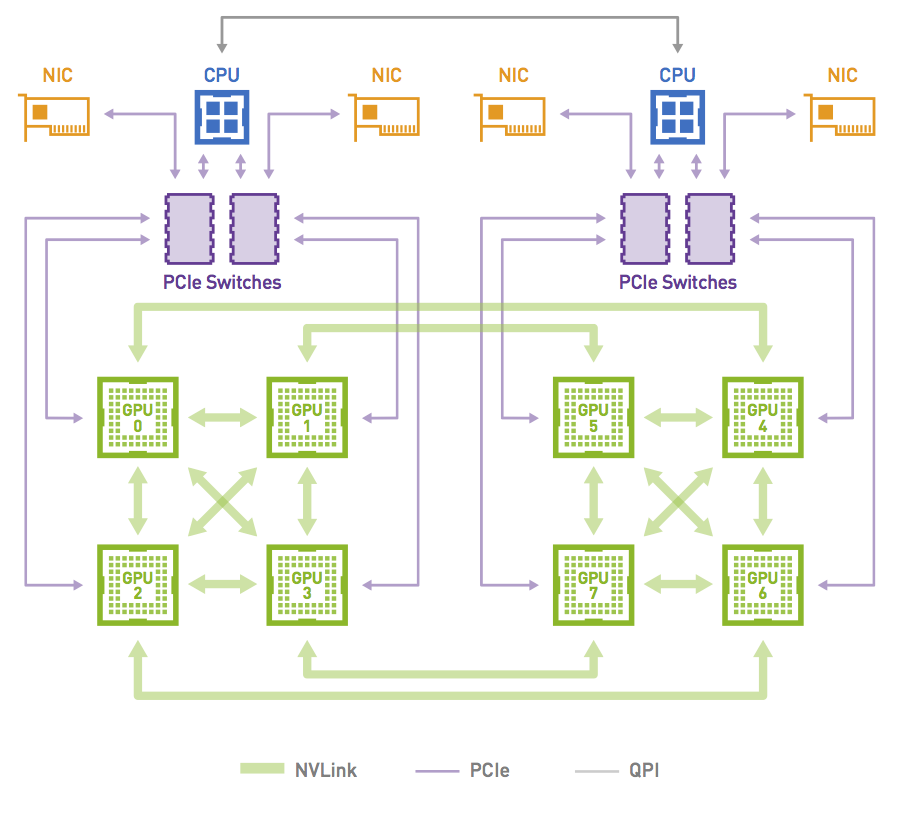
\includegraphics{attachments/scaling/NVLink-DGX1.png}

Each of the NVLink links runs at 20 GBps per direction, higher than PCIe
3.0 x16 (16 GBps for the whole GPU). But the topology is not all-to-all,
and GPUs may not be able to access every other GPU's memory. For
example, GPU0 can't use peer access on GPUs 5, 6 and 7. This makes
implementations using peer access more complex than a full all-to-all
topology. DGX-1 with V100 GPUs increases the NVLink speed to 25 GBps per
direction per lane, and increases the number of lanes per GPU to 6, but
peer accessibility has not been changed. This issue is finally addressed
in DGX-2 with the NVSwitch.

Using a benchmark program to test throughput and latency shows the
following results. \texttt{Self} indicates local GPU accesses,
\texttt{peer} indicates peer accesses, \texttt{host} indicates accesses
to the CPU memory via UVM, and \texttt{all} indicates accesses to all
peer-accessible GPUs. The \texttt{regular} operations access the memory
in continous places by neighboring threads; in CUDA terms, these
operations are coalesced memory accesses. The \texttt{random} operations
access the memory space randomly, and neighboring threads may be
touching memory that are far away from each other; in CUDA terms, these
operations are non-coalesced memory accesses. The memory access patterns
of graph workflows are a mix of both, and one main target of kernel
optimizations is to make the memory accesses as coalesced as possible.
But at the end, depending on the algorithm, some random accesses may be
unavoiable. Random accesses across GPUs are particularly slow.

Throughput in GBps:

\begin{longtable}[]{@{}lrrrr@{}}
\toprule
Operation & Self & Peer & Host & All\tabularnewline
\midrule
\endhead
Regular read & 448.59 & 14.01 & 444.74 & 12.17\tabularnewline
Regular write & 442.98 & 16.21 & 16.18 & 12.17\tabularnewline
Regular update & 248.80 & 11.71 & 0.0028 & 6.00\tabularnewline
Random read & 6.78 & 1.43 & 2.39 & 4.04\tabularnewline
Random write & 6.63 & 1.14 & 3.47E-5 & 3.82\tabularnewline
Random update & 3.44 & 0.83 & 1.92E-5 & 2.08\tabularnewline
\bottomrule
\end{longtable}

Latency in microseconds (us):

\begin{longtable}[]{@{}lrrrr@{}}
\toprule
Operation & Self & Peer & Host & All\tabularnewline
\midrule
\endhead
Regular read & 2.12 & 1.18 & 1.30 & 1.49\tabularnewline
Regular write & 1.74 & 1.00 & 13.83 & 1.01\tabularnewline
Regular update & 2.43 & 1.20 & 79.29 & 1.44\tabularnewline
Random read & 3.11 & 1.08 & 13.61 & 1.40\tabularnewline
Random write & 3.28 & 1.05 & 15.88 & 1.39\tabularnewline
Random update & 5.69 & 1.28 & 21.76 & 1.38\tabularnewline
\bottomrule
\end{longtable}

All the regular throughputs are at least 80\% of their theoretical upper
bounds. The latencies when accessing local GPUs seem odd, but other
latencies look reasonable. It's clear that local regular accesses have
much higher throughput than inter-GPU connections, about 20 to 30 times
from this experiment. The ratio of random accesses are lower, but still
at about 5 times. The implication on the scalabilities of graph
applications is that for scalable behavior, the
local-memory-access-to-communication ratio needs to be at least 10 to 1.
Because most graph implementations are memory bound, the computation
cost is counted by the number of elements accessed by the kernels; this
means the computation to communication ratio should be at least 2.5
operations to 1 byte to exhibit scalable behavior.

Unified virtual memory (UVM) doesn't work as expected for most cases,
instead only when the accesses are read only and the data can be
duplicated on each GPU. Otherwise the throughputs are significantly
lower, caused by memory migration and going over the PCIe interfaces.
The less than 0.5 GBps throughputs from write and update operations via
UVM could possibily caused by problems in the UVM support or the way how
UVM is configured in the benchmark code. It must be noted that, at the
time of testing, the DGX-1 has CUDA 9.1 and NVIDIA driver 390.30
installed, which are more than one year old. A newer CUDA version and
NVIDIA driver could potentially improve the UVM performance. Testing
using V100 GPUs with CUDA 10.0 and NVIDIA driver 410 shows considerablly
better throughputs.

\hypertarget{dgx-2}{%
\subsection{DGX-2}\label{dgx-2}}

The DGX-2 system has a very different NVLink topology: the GPUs are
connected by NVSwitches, and all to all peer accesses are available.

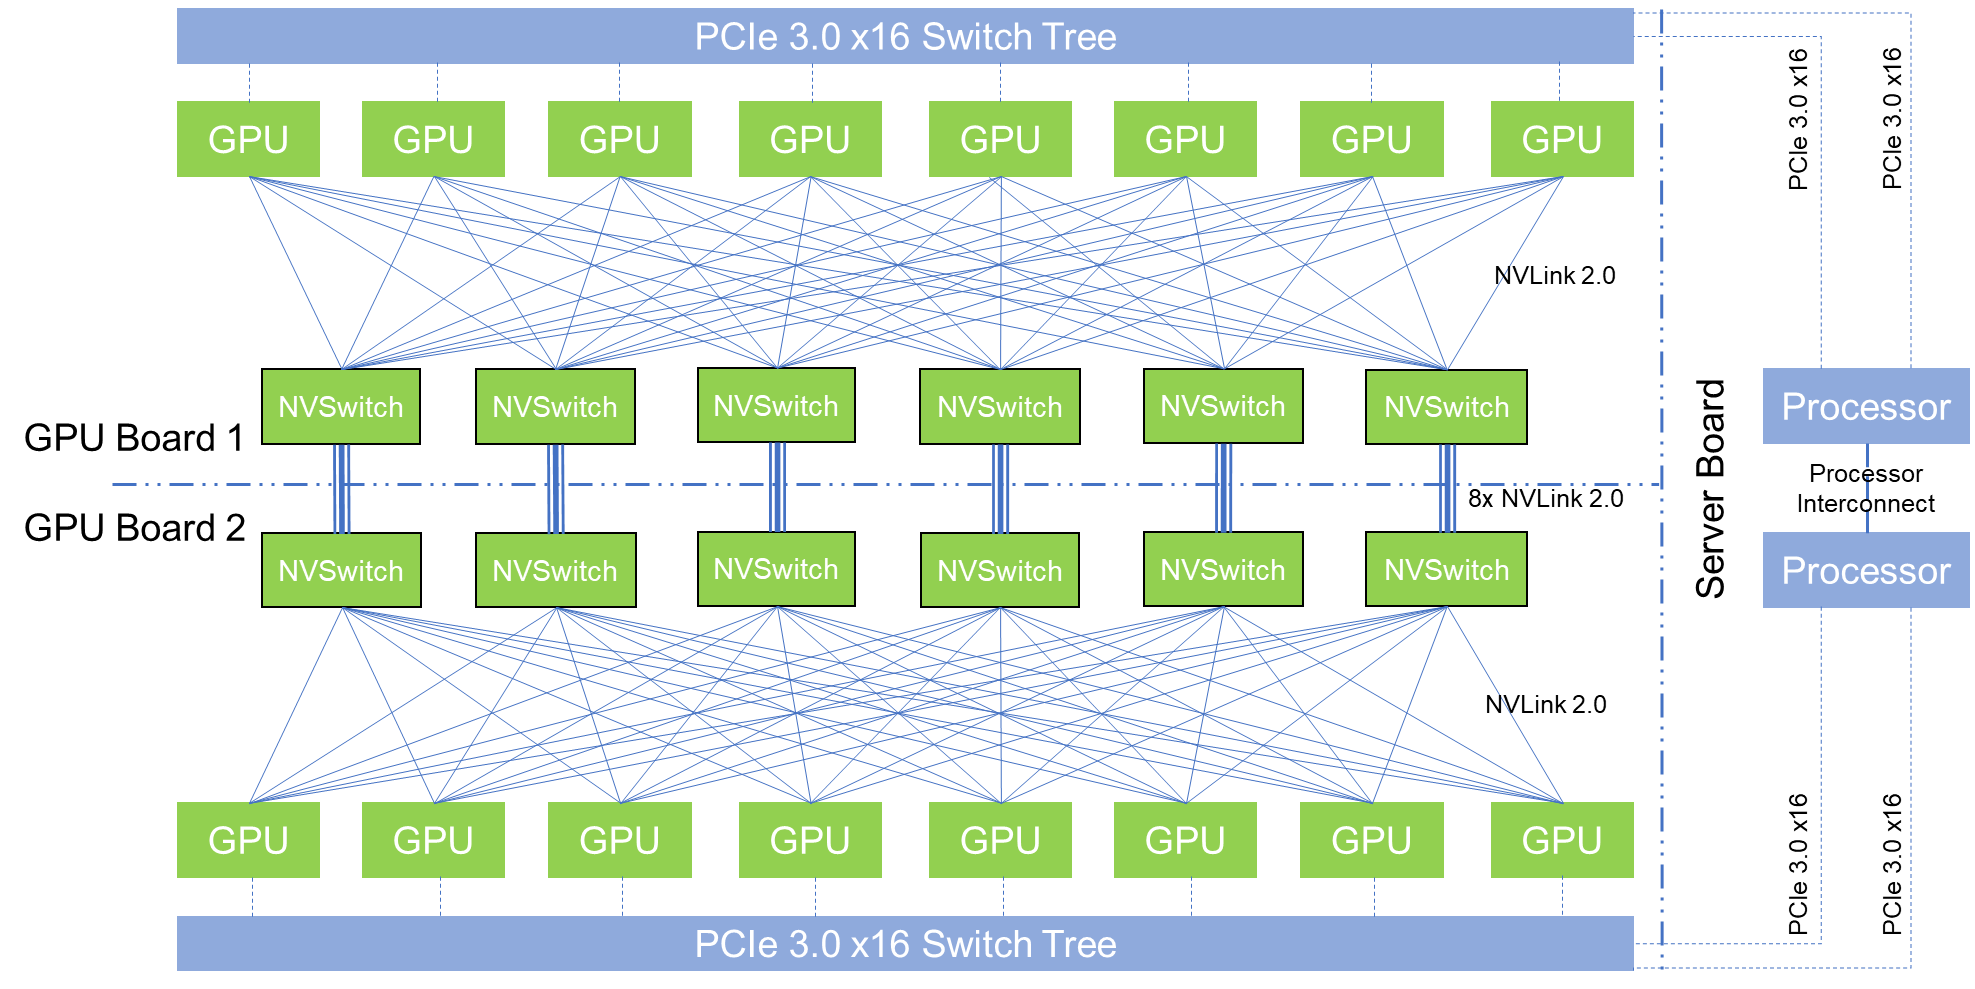
\includegraphics{attachments/scaling/NVLink-DGX2.png}.

At the time of this report, the DGX-2 is hardly available, and not to
us. What we have locally at UC Davis are two Quadro GV100 GPUs directly
connected by 4 NVLink2 lanes. Although the setup is much smaller than
the DGX-2, it still can provide some ideas on how the inter-GPU
communication would perform on the DGX-2.

Throughput in GBps

\begin{longtable}[]{@{}lrrrr@{}}
\toprule
Operation & Self & Peer & Host & All\tabularnewline
\midrule
\endhead
Regular read & 669.68 & 76.74 & 679.52 & 76.72\tabularnewline
Regular write & 590.01 & 85.00 & 170.113 & 76.28\tabularnewline
Regular update & 397.26 & 39.67 & 80.00 & 37.86\tabularnewline
Random read & 17.39 & 7.46 & 17.27 & 10.51\tabularnewline
Random write & 13.25 & 7.96 & 1.23 & 7.24\tabularnewline
Random update & 6.83 & 3.88 & 0.68 & 3.85\tabularnewline
\bottomrule
\end{longtable}

Latency in microsecond (us)

\begin{longtable}[]{@{}lrrrr@{}}
\toprule
Operation & Self & Peer & Host & All\tabularnewline
\midrule
\endhead
Regular read & 0.37 & 0.47 & 0.37 & 0.41\tabularnewline
Regular write & 0.08 & 0.08 & 0.08 & 0.15\tabularnewline
Regular update & 0.37 & 0.47 & 0.43 & 0.41\tabularnewline
Random read & 0.11 & 0.10 & 0.10 & 0.16\tabularnewline
Random write & 0.13 & 0.08 & 0.08 & 0.15\tabularnewline
Random update & 0.15 & 0.09 & 0.09 & 0.17\tabularnewline
\bottomrule
\end{longtable}

On this machine configuration, the local-to-peer memory throughput
ratios, about 8 for regular accesses and about 2 for random accesses,
are much lower than the DGX-1. The decreases are mainly from using all
the 4 lanes for communication, instead of 1 in the DGX-1 cases. If using
only a single lane, the ratios would become 32 and 8, even higher than
the DGX-1. The actual effect from the NVSwitch is still unclear, but
DGX-2 is expected to have similar scalabilities as DGX-1 for graph
applications.

\hypertarget{gpu-clusters}{%
\subsection{GPU clusters}\label{gpu-clusters}}

Going from multiple GPUs within the same node to multiple GPUs across
different nodes significantly decreases the inter-GPU throughput. While
NVLink runs at 80 GBps per direction per GPU for the DGX-1, the
aggregated InfiniBand bandwidth is only 400 Gbps, which is only one
twelfth of the aggregated inter-GPU bandwidth. This means the local
access-to-communication-bandwidth ratio drops an order of magnitude,
making scaling graph applications across nodes a corresponding order of
magnitude harder. Using the same approximation method as the DGX-1, a
graph implementation needs to have 30 operations / local memory
operations for each byte going across the nodes. The implementation
focus may need to switch to communication, rather than local
computation, to achieve a scalable implementation on GPU clusters.

\hypertarget{communication-methods-models}{%
\section{Communication methods /
models}\label{communication-methods-models}}

There are multiple ways to move data between GPUs: explicit movement,
peer accesses, and unified virtual memory (UVM). They have different
performance and implications in implementing graph workflows.

\hypertarget{explicit-data-movement}{%
\subsection{Explicit data movement}\label{explicit-data-movement}}

The most traditional way to communicate is to explicitly move the data:
use \texttt{cudaMemcpyAsync} to copy a block of memory from one GPU to
another. The source and destination GPUs are not required to be peer
accessible. CUDA will automatically select the best route: if GPUs are
peer-accessible, the traffic will go through the inter-GPU connection,
be it NVLink or PCIe; if they are not peer-accessible, the data will be
first copied to CPU memory, and then copied to the destination GPU.

One of the advantage of explicit data movement is throughput.
\texttt{cudaMemcpyAsync} is highly optimized, and the data for
communication are always dense. The throughput should be close to the
hardware limit, if the size of data is not too small, say at least a few
tens of MB. Explicit data movement also isolates local computation and
communication. Because there is no need to consider the data layout or
different access latencies from local or remote data, the implementation
and optimization of computation kernels can be much simpler. It also
enables connection to other communication libraries, such as MPI.

However, explicit memory copy requires that data for communication are
packed in a continuous memory space. For most applications, this means
additional computation to prepare the data. Since the computing power of
GPUs is huge, and graph applications are mostly memory-bound, this extra
computation should only have minimal impact on the running time.

Many graph algorithms are written using the bulk synchronous parallel
(BSP) model: computations are carried out in iterations, and the results
of computation are only guaranteed to be visible after the iteration
boundary. The BSP model provides a natural communication point: at the
iteration boundary. The current Gunrock multi-GPU framework follows the
BSP model.

Depending on the algorithm, there are several communication models that
can be used:

\begin{itemize}
\item
  \textbf{Peer to host GPU} This communication model is used when data
  of a vertex or edge on peer GPUs need to be accumulated / aggregated
  onto the host GPU of the vertex. When the vertex or edge is only
  adjacent to a few GPUs, it may be beneficial to use direct p2p
  communication; when the vertex is adjacent to most GPUs, a
  \texttt{Reduce} from all GPUs to the host GPU may be better.
\item
  \textbf{Host GPU to peers} This is the opposite to the peer-to-host
  model. It propagates data of a vertex or edge from its host GPU to all
  GPUs adjacent to the vertex. Similarly, if the number of adjacent GPUs
  are small, point-to-point communication should do the work; otherwise,
  \texttt{broadcast} from the host GPU may be better.
\item
  \textbf{All reduce} When updates on the same vertex or edge come from
  many GPUs, and the results are needed on many GPUs, \texttt{AllReduce}
  may be the best choice. It can be viewed as an
  \texttt{peers\ to\ host} followed by an \texttt{host\ to\ peers}
  communication. It can also be used without partitioning the graph: it
  works without knowing or assigning a host GPU to an vertex or edge.
\item
  \textbf{Mix all reduce with peers to host GPU or host GPU to peers}
  This is a mix of \texttt{AllReduce} and peer-to-peer communications:
  for vertices or edges that touch a large number of GPUs,
  \texttt{AllReduce} is used; for other vertices or edges, direct
  peer-to-peer communications are used. This communication model is
  coupled with the high / low degree partitioning scheme. The paper
  ``Scalable Breadth-First Search on a GPU Cluster''
  \url{https://escholarship.org/uc/item/9bd842z6} has more details on
  this model.
\end{itemize}

\hypertarget{peer-accesses}{%
\subsection{Peer accesses}\label{peer-accesses}}

If a pair of GPUs is peer-accessible, they can directly dereference each
other's memory pointers within CUDA kernels. This provides a more
asynchronous way for inter-GPU communication: there is no need to wait
for the iteration boundary. Atomic operations are also supported if the
GPUs are connected by NVLink. The implementation can also be kept
simple, since no data preparing and explicit movement is needed. The
throughput is also acceptable, although not as good as explicit
movement.

However, this essentially forces the kernel to work on a NUMA
(non-uniform memory access) domain formed by local and remote GPU
memory. Some kernels optimized under the assumption of a flat memory
domain may not work well. Peer accesses also give up the opportunity to
aggregate local updates on the same vertex or edge before communication,
so the actual communication volume may be larger.

\hypertarget{unified-virtual-memory-uvm}{%
\subsection{Unified virtual memory
(UVM)}\label{unified-virtual-memory-uvm}}

UVM is similar to peer accesses, as it also enables multiple GPUs to
access the same memory space. However, the target memory space is
allocated in the CPU memory. When needed on a GPU, a memory page will be
moved to the GPU's memory via the page fault mechanism. Updates to the
data are cached in GPU memory first, and will eventually be written to
the CPU memory. UVM provides a transparent view of the CPU memory on
GPU, and significantly reduces the coding complexity if running time is
not a concern. It also enables the GPU to process datasets that can't
fit in combined GPU memory without explicitly streaming the data from
CPU to GPU.

But there are some caveats. The actual placement of a memory page/piece
of data relies on hints given by \texttt{cudaMemAdvise}, otherwise it
will need to be fetched from CPU to GPU when first used by any GPU, and
bounces between GPUs when updated by multiple GPUs. The hints
essentially come from partitioning the data, but sometimes there is no
good way to partition, and data bouncing is unavoidable. In the worst
cases, the data can be moved back to CPU, and any further access will
need to go through the slow PCIe bridge again. The performance of UVM is
not as good as explicit data movement or peer accesses; in the worst
cases, it can be a few orders of magnitude slower. When data is larger
than the GPU memory, UVM's throughput drops significantly; as a result,
it's easier to code, but it will be slower than streaming the graph for
datasets larger than GPU memory.

\hypertarget{graph-partitioning-scheme}{%
\section{Graph partitioning scheme}\label{graph-partitioning-scheme}}

Graphs may be cut into smaller pieces to put them onto multiple GPUs.
Duplicating the graph on each may work for some problems, provided the
graph is not too large; but duplication is not suitable for all
problems, and does not scale in graph size. Graph partitioning is a
long-lasting research topic, and we decided to use existing
partitioners, such as Metis, instead of implementing some complicated
ones of our own. A large number of graphs, especially those with high
connectivities, are really difficult to partition; our results suggest
that random partitioning works quite well in terms of time taken by the
partitioner, load balancing, programming simplicity and still manageable
communication cost. By default, Gunrock uses the random partitioner.

What makes a bigger difference is the partitioning scheme: whether the
graph is partitioned in 1 dimension, 2 dimensions, or differently for
low and high degree vertices.

\hypertarget{d-partitioning}{%
\subsection{1D partitioning}\label{d-partitioning}}

1D partitioning distributes the edges in a graph either by the source
vertices or the destination vertices. It's simple to work with, and
scales well when the number of GPUs are small. It should still work on
the DGX-1 with 8 GPUs for a large number of graph applications. But that
may approach 1D partitioning's scalability limit.

\hypertarget{d-partitioning-1}{%
\subsection{2D partitioning}\label{d-partitioning-1}}

2D partitioning distributes the edges by both the source and the
destination vertices. When a graph is visualized in a dense matrix
representation, 2D partitioning is like cutting the matrix by a 2D grid.
8 GPUs in the DGX-1 may be too small for 2D partitioning to be useful;
it may worth trying out on DGX-2 with 16 GPUs. 2D partitioning of sparse
graphs may create significant load imbalance between partitions.

\hypertarget{highlow-degree-partitioning}{%
\subsection{High/low degree
partitioning}\label{highlow-degree-partitioning}}

The main idea of high/low degree partitioning is simple: for vertices
with low out-degrees and their outgoing edges, distribute edges based on
their source vertices; for vertices with high out-degrees and their
outgoing edges, distribute edges based on the destination vertices; if
both vertices have high out-degrees, distribute the edge based on the
one with lower degree. The result is that low degree vertices are only
adjacent to very few GPUs, while high degree vertices' edges are
scattered among all GPUs. Graph applications scale very well when using
the p2p communication model for low degree vertices, and the
\texttt{AllReduce} model for high degree vertices.

\hypertarget{scaling-of-the-hive-applications}{%
\section{Scaling of the HIVE
applications}\label{scaling-of-the-hive-applications}}

The target platform DGX-1 has 8 GPUs. Although that is more than we
normally see for single scaling studies, the simple 1D graph
partitioning scheme should (in general) still work. The marginal
performance improvement by using more GPUs may be insignificant at this
scale, and a small number of applications might even see performance
decreases with some datasets. However, the 1D partitioning makes the
scaling analysis simple and easily understandable. If other partitioning
schemes could work better for a specific application, it would be noted.

\hypertarget{how-scaling-is-considered}{%
\subsection{How scaling is considered}\label{how-scaling-is-considered}}

The bandwidth of NVLink is much faster than PCIe 3.0: 20x3 and 25x6 GBps
bidirectionally for each Tesla P100 and V100 GPUs respectively in an
DGX-1. But compared to the several TFLOPs computing power and several
hundred GBps device bandwidth, the inter-GPU bandwidth is still
considerably less. For any application to have good scalability, the
communication time should be able to be either: 1) hidden by overlap
with computation, or 2) kept as a small portion of the computation. The
computation-to-communication ratio is a good indicator to predict the
scalability: a higher ratio means better scalability. Specific to the
DGX-1 system with P100 GPUs, a ratio larger than about 10 to 1 is
expected for an app to have at least marginal scalability. For GPUs
newer than P100, the computation power and memory bandwidth improve
faster than interconnect bandwidth, so the compute-to-communicate ratio
needs to grow even more to start seeing positive scaling.

\hypertarget{community-detection-louvain-2}{%
\subsection{Community Detection
(Louvain)}\label{community-detection-louvain-2}}

The main and most time-consuming part of the Louvain algorithm is the
modularity optimization iterations. The aggregated edge weights between
vertices and their respective adjacent communities, as well as the
outgoing edge weights of each community, are needed for the modularity
optimization. The vertex-community weights can be computed locally, if
the community assignments of all neighbors of local vertices are
available; to achieve this, a vertex needs to broadcast its new
community when the assignment changes. The per-community outgoing edge
weights can be computed by \texttt{AllReduce} across all GPUs. The
modularity optimization with inter-GPU communication can be done as:

\begin{verbatim}
Do
    Local modularity optimization;
    Broadcast updated community assignments of local vertices;
    local_weights_community2any := sums(local edges from an community);
    weights_community2any := AllReduce(local_weights_community2any, sum);
While iterations stop condition not met
\end{verbatim}

The local computation cost is on the order of \(O(|E| + |V|)/p\), but
with a large constant hidden by the \(O()\) notation. From experiments,
the constant factor is about 10, considering the cost of sort or the
random memory access penalty of hash table. The community assignment
broadcast has a cost of \textbar{}V\textbar{} x 4 bytes, and the
`AllReduce' costs \(2|V| \times 8\) bytes. These communication costs are
the upper bound, assuming there are \(|V|\) communities, and all
vertices update their community assignments. In practice, the
communication cost can be much lower, depending on the dataset.

The graph contraction can be done as below on multiple GPUs:

\begin{verbatim}
temp_graph := Contract the local sub-graph based on community assignments;
Send edges <v, u, w> in temp_graph to host_GPU(v);
Merge received edges and form the new local sub-graph;
\end{verbatim}

In the worst case, assuming the number of edges in the contracted graph
is \(|E'|\), the communication cost could be \(|E'| \times 8\) bytes,
with the computation cost at about \(5|E|/p + |E'|\). For most datasets,
the size reduction of graph from the contraction step is significant, so
the memory needed to receive edges from the peer GPUs is manageable;
however, if \(|E'|\) is large, it can be significant and may run out of
GPU memory.

\emph{Summary of Louvain multi-GPU scaling}

Because the modularity optimization runs multiple iterations before each
graph contraction phase, the computation and communication of modularity
optimization is dominant.

\begin{longtable}[]{@{}llllll@{}}
\toprule
Parts & Comp cost & Comm cost & Comp/comm ratio & Scalability & Memory
usage (B)\tabularnewline
\midrule
\endhead
Modularity optim. & \(10(E + V) /p\) & \(20V\) bytes & \(E/p : 2V\) &
Okay & \(88E/p + 12V\)\tabularnewline
Graph contraction & \(5E / p + E'\) & \(8E'\) bytes &
\(5E/p + E' : 8E'\) & Hard & \(16E'\)\tabularnewline
Louvain & \(10(E + V) / p\) & \(20V\) bytes & \(E/p : 2V\) & Okay &
\(88E/p + 12V + 16E'\)\tabularnewline
\bottomrule
\end{longtable}

Louvain could be hard to implement on multiple GPUs, especially for the
graph contraction phase, as it forms a new graph and distributes it
across the GPUs. But the scalability should be okay.

\hypertarget{graphsage-2}{%
\subsection{GraphSAGE}\label{graphsage-2}}

The main memory usage and computation of SAGE are related to the
features of vertices. While directly accessing the feature data of
neighbors via peer access is possible and memory-efficient, it will
create a huge amount of inter-GPU traffic that makes SAGE unscalable in
terms of running time. Using UVM to store the feature data is also
possible, but that will move the traffic from inter-GPU to the GPU-CPU
connection, which is even less desirable. Although there is a risk of
using up the GPU memory, especially on graphs that have high
connectivity, a more scalable way is to duplicate the feature data of
neighboring vertices. Depending on the graph size and the size of
features, not all of the above data distribution schemes are applicable.
The following analysis focuses on the feature duplication scheme, with
other schemes' results in the summary table.

SAGE can be separated into three parts, depending on whether the
computation and data access is source-centric or child-centric.

\begin{verbatim}
// Part1: Select the children
For each source in local batch:
    Select num_children_per_source children form source's neighbors;
    Send <source, child> pairs to host_GPU(child);

// Part2: Child-centric computation
For each received <source, child> pair:
    child_feature = feature[child];
    send child_feature to host_GPU(source);

    feature_sums := {0};
    For i from 1 to num_leaves_per_child:
        Select a leaf from child's neighbors;
        leaves_feature += feature[leaf];
    child_temp = L2_normalize( concatenate(
        feature[child] * Wf1, leaves_feature * Wa1));
    send child_temp to host_GPU(source);

// Part3: Source-centric computation
For each source in local batch:
    children_feature := sum(received child_feature);
    children_temp := sum(received child_temp);
    source_temp := L2_normalize( concatenate(
        feature[source] * Wf1, children_feature * Wa1));

    source_result := L2_normalize( concatenate(
        source_temp * Wf2, children_temp * Wa2));
\end{verbatim}

Assume the size of local batch is B, the number of children per source
is C, the number of leaves per child is L, and the feature length per
vertex is F. Dimensions of 2D matrices are noted as (x, y). The
computation and communication costs for each part are:

\begin{verbatim}
Part 1, computation  : B x C.
Part 1, communication: B x C x 8 bytes.
Part 2, computation  : B x C x F + B x C x (F + L x F + F x (Wf1.y + Wa1.y)).
Part 2, communication: B x C x (F + Wf1.y + Wa1.y) x 4 bytes.
Part 3, computation  : B x (C x (F + Wf1.y + Wa1.y) + F x (Wf1.y + Wa1.y) +
                       (Wf1.y + Wa1.y) x (Wf2.y + Wa2.y)).
Part 3, communication: 0.
\end{verbatim}

For Part 2's communication, if C is larger than about 2p, using
\texttt{AllReduce} to sum up \texttt{child\_feature} and
\texttt{child\_temp} for each source will cost less, at
\(B \times (F + \textrm{Wf1}.y + \textrm{Wa1}.y) \times 2p \times 4\)
bytes.

\emph{Summary of Graph SAGE multi-GPU scaling}

\begin{longtable}[]{@{}lllll@{}}
\toprule
\begin{minipage}[b]{0.18\columnwidth}\raggedright
Parts\strut
\end{minipage} & \begin{minipage}[b]{0.14\columnwidth}\raggedright
Computation cost\strut
\end{minipage} & \begin{minipage}[b]{0.25\columnwidth}\raggedright
Communication cost (Bytes)\strut
\end{minipage} & \begin{minipage}[b]{0.18\columnwidth}\raggedright
Comp. to comm. ratio\strut
\end{minipage} & \begin{minipage}[b]{0.10\columnwidth}\raggedright
Scalability\strut
\end{minipage}\tabularnewline
\midrule
\endhead
\begin{minipage}[t]{0.18\columnwidth}\raggedright
\textbf{Feature duplication}\strut
\end{minipage} & \begin{minipage}[t]{0.14\columnwidth}\raggedright
\strut
\end{minipage} & \begin{minipage}[t]{0.25\columnwidth}\raggedright
\strut
\end{minipage} & \begin{minipage}[t]{0.18\columnwidth}\raggedright
\strut
\end{minipage} & \begin{minipage}[t]{0.10\columnwidth}\raggedright
\strut
\end{minipage}\tabularnewline
\begin{minipage}[t]{0.18\columnwidth}\raggedright
Children selection\strut
\end{minipage} & \begin{minipage}[t]{0.14\columnwidth}\raggedright
\(BC\)\strut
\end{minipage} & \begin{minipage}[t]{0.25\columnwidth}\raggedright
\(8BC\)\strut
\end{minipage} & \begin{minipage}[t]{0.18\columnwidth}\raggedright
1 : 8\strut
\end{minipage} & \begin{minipage}[t]{0.10\columnwidth}\raggedright
Poor\strut
\end{minipage}\tabularnewline
\begin{minipage}[t]{0.18\columnwidth}\raggedright
Child-centric comp.\strut
\end{minipage} & \begin{minipage}[t]{0.14\columnwidth}\raggedright
\(BCF \cdot (2 + L + \textrm{Wf1}.y + \textrm{Wa1}.y)\)\strut
\end{minipage} & \begin{minipage}[t]{0.25\columnwidth}\raggedright
\(4B \cdot (F + \textrm{Wf1}.y + \textrm{Wa1}.y) \cdot \min(C, 2p)\)\strut
\end{minipage} & \begin{minipage}[t]{0.18\columnwidth}\raggedright
\(\sim CF : \min(C, 2p) \cdot 4\)\strut
\end{minipage} & \begin{minipage}[t]{0.10\columnwidth}\raggedright
Good\strut
\end{minipage}\tabularnewline
\begin{minipage}[t]{0.18\columnwidth}\raggedright
Source-centric comp.\strut
\end{minipage} & \begin{minipage}[t]{0.14\columnwidth}\raggedright
\(B \cdot (CF + (\textrm{Wf1}.y + \textrm{Wa1}.y) \cdot (C + F + \textrm{Wf2}.y + \textrm{Wa2}.y)\)\strut
\end{minipage} & \begin{minipage}[t]{0.25\columnwidth}\raggedright
0\strut
\end{minipage} & \begin{minipage}[t]{0.18\columnwidth}\raggedright
N.A.\strut
\end{minipage} & \begin{minipage}[t]{0.10\columnwidth}\raggedright
N.A.\strut
\end{minipage}\tabularnewline
\begin{minipage}[t]{0.18\columnwidth}\raggedright
Graph SAGE\strut
\end{minipage} & \begin{minipage}[t]{0.14\columnwidth}\raggedright
\(B \cdot (C + 3CF + 3LCF + (\textrm{Wf1}.y + \textrm{Wa1}.y) \cdot (CF + C + F + \textrm{Wf2}.y + \textrm{Wa2}.y))\)\strut
\end{minipage} & \begin{minipage}[t]{0.25\columnwidth}\raggedright
\(8BC + 4B \cdot (F + \textrm{Wf1}.y + \textrm{Wa1}.y) \cdot \min(C, 2p)\)\strut
\end{minipage} & \begin{minipage}[t]{0.18\columnwidth}\raggedright
at least \(\sim CF : \min(C, 2p) \cdot 4\)\strut
\end{minipage} & \begin{minipage}[t]{0.10\columnwidth}\raggedright
Good\strut
\end{minipage}\tabularnewline
\begin{minipage}[t]{0.18\columnwidth}\raggedright
\strut
\end{minipage} & \begin{minipage}[t]{0.14\columnwidth}\raggedright
\strut
\end{minipage} & \begin{minipage}[t]{0.25\columnwidth}\raggedright
\strut
\end{minipage} & \begin{minipage}[t]{0.18\columnwidth}\raggedright
\strut
\end{minipage} & \begin{minipage}[t]{0.10\columnwidth}\raggedright
\strut
\end{minipage}\tabularnewline
\begin{minipage}[t]{0.18\columnwidth}\raggedright
\textbf{Direct feature access}\strut
\end{minipage} & \begin{minipage}[t]{0.14\columnwidth}\raggedright
\strut
\end{minipage} & \begin{minipage}[t]{0.25\columnwidth}\raggedright
\strut
\end{minipage} & \begin{minipage}[t]{0.18\columnwidth}\raggedright
\strut
\end{minipage} & \begin{minipage}[t]{0.10\columnwidth}\raggedright
\strut
\end{minipage}\tabularnewline
\begin{minipage}[t]{0.18\columnwidth}\raggedright
Child-centric comp.\strut
\end{minipage} & \begin{minipage}[t]{0.14\columnwidth}\raggedright
\(BCF \cdot (2 + L + \textrm{Wf1}.y + \textrm{Wa1}.y)\)\strut
\end{minipage} & \begin{minipage}[t]{0.25\columnwidth}\raggedright
\(4B \cdot ((F + \textrm{Wf1}.y + \textrm{Wa1}.y) \cdot \min(C, 2p) + CLF)\)\strut
\end{minipage} & \begin{minipage}[t]{0.18\columnwidth}\raggedright
\(\sim (2 + L + \textrm{Wf1}.y + \textrm{Wa1}.y) : 4L\)\strut
\end{minipage} & \begin{minipage}[t]{0.10\columnwidth}\raggedright
poor\strut
\end{minipage}\tabularnewline
\begin{minipage}[t]{0.18\columnwidth}\raggedright
Graph SAGE\strut
\end{minipage} & \begin{minipage}[t]{0.14\columnwidth}\raggedright
\(B \cdot (C + 3CF + 3LCF + (\textrm{Wf1}.y + \textrm{Wa1}.y) \cdot (CF + C + F + \textrm{Wf2}.y + \textrm{Wa2}.y))\)\strut
\end{minipage} & \begin{minipage}[t]{0.25\columnwidth}\raggedright
\(8BC + 4B \cdot (F + \textrm{Wf1}.y + \textrm{Wa1}.y) \cdot \min(C, 2p) + 4BCFL\)\strut
\end{minipage} & \begin{minipage}[t]{0.18\columnwidth}\raggedright
\(\sim (2 + L + \textrm{Wf1}.y + \textrm{Wa1}.y) : 4L\)\strut
\end{minipage} & \begin{minipage}[t]{0.10\columnwidth}\raggedright
poor\strut
\end{minipage}\tabularnewline
\begin{minipage}[t]{0.18\columnwidth}\raggedright
\strut
\end{minipage} & \begin{minipage}[t]{0.14\columnwidth}\raggedright
\strut
\end{minipage} & \begin{minipage}[t]{0.25\columnwidth}\raggedright
\strut
\end{minipage} & \begin{minipage}[t]{0.18\columnwidth}\raggedright
\strut
\end{minipage} & \begin{minipage}[t]{0.10\columnwidth}\raggedright
\strut
\end{minipage}\tabularnewline
\begin{minipage}[t]{0.18\columnwidth}\raggedright
\textbf{Feature in UVM}\strut
\end{minipage} & \begin{minipage}[t]{0.14\columnwidth}\raggedright
\strut
\end{minipage} & \begin{minipage}[t]{0.25\columnwidth}\raggedright
\strut
\end{minipage} & \begin{minipage}[t]{0.18\columnwidth}\raggedright
\strut
\end{minipage} & \begin{minipage}[t]{0.10\columnwidth}\raggedright
\strut
\end{minipage}\tabularnewline
\begin{minipage}[t]{0.18\columnwidth}\raggedright
Child-centric comp.\strut
\end{minipage} & \begin{minipage}[t]{0.14\columnwidth}\raggedright
\(BCF \cdot (2 + L + \textrm{Wf1}.y + \textrm{Wa1}.y)\)\strut
\end{minipage} & \begin{minipage}[t]{0.25\columnwidth}\raggedright
\(4B \cdot (F + \textrm{Wf1}.y + \textrm{Wa1}.y) \cdot \min(C, 2p)\)
bytes over GPU-GPU + \(4BCLF\) bytes over GPU-CPU\strut
\end{minipage} & \begin{minipage}[t]{0.18\columnwidth}\raggedright
\(\sim (2 + L + \textrm{Wf1}.y + \textrm{ a1}.y) : 4L\) over
GPU-CPU\strut
\end{minipage} & \begin{minipage}[t]{0.10\columnwidth}\raggedright
very poor\strut
\end{minipage}\tabularnewline
\begin{minipage}[t]{0.18\columnwidth}\raggedright
Graph SAGE\strut
\end{minipage} & \begin{minipage}[t]{0.14\columnwidth}\raggedright
\(B \cdot (C + 3CF + 3LCF + (\textrm{Wf1}.y + \textrm{Wa1}.y) \cdot (CF + C + F + \textrm{Wf2}.y + \textrm{Wa2}.y))\)\strut
\end{minipage} & \begin{minipage}[t]{0.25\columnwidth}\raggedright
\(8BC + 4B \cdot (F + \textrm{Wf1}.y + \textrm{Wa1}.y) \cdot \min(C, 2p)\)
bytes over GPU-GPU + \(4BCFL\) bytes over GPU-CPU\strut
\end{minipage} & \begin{minipage}[t]{0.18\columnwidth}\raggedright
\(\sim (2 + L + \textrm{Wf1}.y + \textrm{Wa1}.y) : 4L\) over
GPU-CPU\strut
\end{minipage} & \begin{minipage}[t]{0.10\columnwidth}\raggedright
very poor\strut
\end{minipage}\tabularnewline
\bottomrule
\end{longtable}

When the number of features is at least several tens, the computation
workload will be much more than communication, and SAGE should have good
scalability. Implementation should be easy, as only simple p2p or
AllReduce communication models are used. If memory usage is an issue,
falling back to peer-access or UVM will result in very poor scalability;
problem segmentation (i.e,. only process portion of the graph at a time)
may be necessary to have a scalable implementation for large graphs, but
that will be quite complex.

\hypertarget{random-walks-and-graph-search}{%
\subsection{Random walks and graph
search}\label{random-walks-and-graph-search}}

If the graph can be duplicated on each GPU, the random walk multi-GPU
implementation is trivial: just do a subset of the walks on each GPU.
The scalability will be perfect, as there is no communication involved
at all.

A more interesting multi-GPU implementation would be when the graph is
distributed across the GPUs. In this case, each step of a walk not only
needs to send the \texttt{\textless{}walk\#,\ step\#,\ v\textgreater{}}
information to \texttt{host\_GPU(v)}, but also to the GPU that stores
the result for such walk.

\begin{verbatim}
For each walk starting from local vertex v:
    Store v for ;
    Select a neighbor u of v;
    Store u for ;
    Send  to host_GPU(u) for visit;

Repeat until all steps of walks finished:
    For each received  for visit:
        Select a neighbor u of v;
        Send  to host_GPU(u) for visit;
        Send  to host_GPU_walk(walk#) for record;

    For each received  for record:
        Store v for ;
\end{verbatim}

Using W as the number of walks, for each step, we have

\begin{longtable}[]{@{}lllll@{}}
\toprule
Parts & Comp. cost & Comm. cost & Comp/comm ratio &
Scalability\tabularnewline
\midrule
\endhead
Random walk & \(W/p\) & \(W/p \cdot 24\) bytes & \(1 : 24\) & very
poor\tabularnewline
\bottomrule
\end{longtable}

Graph search is very similar to random walk, except that instead of
randomly selecting any neighbor, it selects the neighbor with the
highest score (when using the \texttt{greedy} strategy), or with
probabilities proportional to the neighbors' scores (when using the
\texttt{stochastic\_greedy} strategy). For the \texttt{greedy} strategy,
a straightforward implementation, when reaching a vertex, goes through
the whole neighbor list of thatsuch vertex and finds the one with
maximum score. A more optimized implementation could perform a pre-visit
to find the neighbor with maximum scored neighbor, with a cost of
\(E/p\); during the random walk process, the maximum scored neighbor
will be known without going through the neighbor list.

For the \texttt{stochastic\_greedy} strategy, the straightforward
implementation would also go through all the neighbors, selecting one
based on their scores and a random number. Preprocessing can also help:
perform a scan on the scores of each vertex's neighbor list, with a cost
of \(E/p\); during the random walk, a binary search would be sufficient
to select a neighbor, with weighted probabilities.

The cost analysis, depending on the walk strategy and optimization,
results in:

\begin{longtable}[]{@{}lllll@{}}
\toprule
\begin{minipage}[b]{0.18\columnwidth}\raggedright
Strategy\strut
\end{minipage} & \begin{minipage}[b]{0.23\columnwidth}\raggedright
Comp. cost\strut
\end{minipage} & \begin{minipage}[b]{0.17\columnwidth}\raggedright
Comm. cost\strut
\end{minipage} & \begin{minipage}[b]{0.16\columnwidth}\raggedright
Comp/comm ratio\strut
\end{minipage} & \begin{minipage}[b]{0.12\columnwidth}\raggedright
Scalability\strut
\end{minipage}\tabularnewline
\midrule
\endhead
\begin{minipage}[t]{0.18\columnwidth}\raggedright
Uniform\strut
\end{minipage} & \begin{minipage}[t]{0.23\columnwidth}\raggedright
\(W/p\)\strut
\end{minipage} & \begin{minipage}[t]{0.17\columnwidth}\raggedright
\(W/p \cdot 24\) bytes\strut
\end{minipage} & \begin{minipage}[t]{0.16\columnwidth}\raggedright
\(1 : 24\)\strut
\end{minipage} & \begin{minipage}[t]{0.12\columnwidth}\raggedright
Very poor\strut
\end{minipage}\tabularnewline
\begin{minipage}[t]{0.18\columnwidth}\raggedright
Greedy\strut
\end{minipage} & \begin{minipage}[t]{0.23\columnwidth}\raggedright
Straightforward: \(dW/p\)\strut
\end{minipage} & \begin{minipage}[t]{0.17\columnwidth}\raggedright
\(W/p \cdot 24\) bytes\strut
\end{minipage} & \begin{minipage}[t]{0.16\columnwidth}\raggedright
\(d : 24\)\strut
\end{minipage} & \begin{minipage}[t]{0.12\columnwidth}\raggedright
Poor\strut
\end{minipage}\tabularnewline
\begin{minipage}[t]{0.18\columnwidth}\raggedright
Greedy\strut
\end{minipage} & \begin{minipage}[t]{0.23\columnwidth}\raggedright
Pre-visit: \(W/p\)\strut
\end{minipage} & \begin{minipage}[t]{0.17\columnwidth}\raggedright
\(W/p \cdot 24\) bytes\strut
\end{minipage} & \begin{minipage}[t]{0.16\columnwidth}\raggedright
\(1 : 24\)\strut
\end{minipage} & \begin{minipage}[t]{0.12\columnwidth}\raggedright
Very poor\strut
\end{minipage}\tabularnewline
\begin{minipage}[t]{0.18\columnwidth}\raggedright
Stochastic Greedy\strut
\end{minipage} & \begin{minipage}[t]{0.23\columnwidth}\raggedright
Straightforward: \(dW/p\)\strut
\end{minipage} & \begin{minipage}[t]{0.17\columnwidth}\raggedright
\(W/p \cdot 24\) bytes\strut
\end{minipage} & \begin{minipage}[t]{0.16\columnwidth}\raggedright
\(d : 24\)\strut
\end{minipage} & \begin{minipage}[t]{0.12\columnwidth}\raggedright
Poor\strut
\end{minipage}\tabularnewline
\begin{minipage}[t]{0.18\columnwidth}\raggedright
Stochastic Greedy\strut
\end{minipage} & \begin{minipage}[t]{0.23\columnwidth}\raggedright
Pre-visit: \(log(d)W/p\)\strut
\end{minipage} & \begin{minipage}[t]{0.17\columnwidth}\raggedright
\(W/p \cdot 24\) bytes\strut
\end{minipage} & \begin{minipage}[t]{0.16\columnwidth}\raggedright
\(log(d) : 24\)\strut
\end{minipage} & \begin{minipage}[t]{0.12\columnwidth}\raggedright
Very poor\strut
\end{minipage}\tabularnewline
\bottomrule
\end{longtable}

If the selection of a neighbor is weighted-random, instead of
uniformly-random, it will increase the computation workload to Wd /p,
where d is the average degree of vertices in the graph. As a result, the
computation-to-communication ratio will increase to d:24; for most
graphs, this is still not high enough to have good scalability.

\hypertarget{geolocation-2}{%
\subsection{Geolocation}\label{geolocation-2}}

In each iteration, Geolocation updates a vertex's location based on its
neighbors. For multiple GPUs, neighboring vertices's location
information needs to be available, either by direct access, UVM, or
explicit data movement. The following shows how explicit data movement
can be implemented.

\begin{verbatim}
Do
    Local geo location updates on local vertices;
    Broadcast local vertices' updates;
While no more update
\end{verbatim}

The computation cost is on the order of O(\textbar{}E\textbar{}/p), if
in each iteration all vertices are looking for possible location updates
from neighbors. Because the spatial median function has a lot of
mathematical computation inside, particularly a haversine() for each
edge, the constant factor hidden by O() is large; for simplicity, 100 is
used as the constant factor here. Assuming that we broadcast every
vertex's location gives the upper bound of communication, but in
reality, the communication should be much less, because 1) not every
vertex updates its location every iteration and 2) vertices may not have
neighbors on each GPU, so instead of broadcast, p2p communication may be
used to reduce the communication cost, especially when the graph
connectivity is low.

\begin{longtable}[]{@{}lllll@{}}
\toprule
Comm. method & Comp. cost & Comm. cost & Comp/comm ratio &
Scalability\tabularnewline
\midrule
\endhead
Explicit movement & \(100E/p\) & \(2V \cdot 8\) bytes & \(25E/p : 4V\) &
Okay\tabularnewline
UVM or peer access & \(100E/p\) & \(E/p \cdot 8\) bytes & \(25 : 1\) &
Good\tabularnewline
\bottomrule
\end{longtable}

\hypertarget{vertex-nomination-2}{%
\subsection{Vertex Nomination}\label{vertex-nomination-2}}

Vertex nomination is very similar to a single source shortest path
(SSSP) problem, except it starts from a group of vertices, instead of a
single source. One possible multi-GPU implementation is:

\begin{verbatim}
Set the starting vertex / vertices;
While has new distance updates
    For each local vertex v with distance update:
        For each edge <v, u, w> of vertex v:
            new_distance := distance[v] + w;
            if (distance[u] > new_distance)
                distance[u] = new_distance;

    For each u with distance update:
        Send <u, distance[u]> to host_GPU(u);
\end{verbatim}

Assuming on average, each vertex has its distance updated \texttt{a}
times, and the average degree of vertices is \texttt{d}, the computation
and the communication costs are:

\begin{longtable}[]{@{}lllll@{}}
\toprule
\begin{minipage}[b]{0.14\columnwidth}\raggedright
Parts\strut
\end{minipage} & \begin{minipage}[b]{0.11\columnwidth}\raggedright
Comp. cost\strut
\end{minipage} & \begin{minipage}[b]{0.28\columnwidth}\raggedright
Comm. cost\strut
\end{minipage} & \begin{minipage}[b]{0.21\columnwidth}\raggedright
Comp/comm ratio\strut
\end{minipage} & \begin{minipage}[b]{0.12\columnwidth}\raggedright
Scalability\strut
\end{minipage}\tabularnewline
\midrule
\endhead
\begin{minipage}[t]{0.14\columnwidth}\raggedright
Vertex nomination\strut
\end{minipage} & \begin{minipage}[t]{0.11\columnwidth}\raggedright
\(aE/p\)\strut
\end{minipage} & \begin{minipage}[t]{0.28\columnwidth}\raggedright
\(aV/p \cdot \min(d, p) \cdot 8\) bytes\strut
\end{minipage} & \begin{minipage}[t]{0.21\columnwidth}\raggedright
\(E : 8V \cdot \min(d, p)\)\strut
\end{minipage} & \begin{minipage}[t]{0.12\columnwidth}\raggedright
Okay\strut
\end{minipage}\tabularnewline
\bottomrule
\end{longtable}

The \(\min(d, p)\) part in the communication cost comes from update
aggregation on each GPU: when a vertex has more than one distance
update, only the smallest is sent out; a vertex that has a lot of
neighbors and is connected to all GPUs has its communication cost capped
by \(p \times 8\) bytes.

\hypertarget{scan-statistics}{%
\subsection{Scan Statistics}\label{scan-statistics}}

Scan statistics is essentially triangle counting (TC) for each vertex
plus a simple post-processing step. The current Gunrock TC
implementation is intersection-based: for an edge
\texttt{\textless{}v,\ u\textgreater{}}, intersecting
\texttt{neighbors{[}u{]}} and \texttt{neighbors{[}v{]}} gives the number
of triangles including \texttt{edge\ \textless{}v,\ u\textgreater{}}.
This neighborhood-intersection-based algorithm only works if the
neighborhood of end points of all edges for which we need to count
triangles can reside in the memory of a single GPU. For graphs with low
connectivities, such as road networks and meshes, it is still possible
to partition the graph; for graphs with high connectivity, such as
social networks or some web graphs, it's almost impossible to partition
the graph, and any sizable partition of the graph may touch a large
portion of vertices of the graph. As a result, for general graphs, the
intersection-based algorithm requires the graph can be duplicated on
each GPU. Under this condition, the multi-GPU implementation is trivial:
only count triangles for a subset of edges on each GPU, and no
communication is involved.

A more distributed-friendly TC algorithm is wedge-checking-based
(\url{https://e-reports-ext.llnl.gov/pdf/890544.pdf}). The main idea is
this: for each triangle A-B-C, where
\texttt{degree(A)\ \textgreater{}=\ degree(B)\ \textgreater{}=\ degree(C)},
both A and B are in C's neighborhood, and A is in B's neighborhood; when
testing for possible triangle D-E-F, with
\texttt{degree(D)\ \textgreater{}=\ degree(E)\ \textgreater{}=\ degree(F)},
the wedge (two edges that share the same end point) that needs to be
checked is D-E, and the checking can be simply done by verifying whether
D is in E's neighborhood. As this algorithm is designed for distributed
systems, it should be well-suited for multi-GPU system. The ordering
requirements are imposed to reduce the number of wedge checks and to
balance the workload. The multi-GPU pseudo code is:

\begin{verbatim}
For each local edge < v, u >:
    If (degree(v) > degree(u)) continue;
    For each neighbor w of v:
        If (degree(v) > degree(w)) continue;
        If (degree(u) > degree(w)) continue;
        Send tuple <u, w, v> to host_GPU(u) for checking;

For each received tuple < u, w, v >:
    If (w in u's neighbor list):
        triangles[u] ++;
        triangles[w] ++;
        triangles[v] ++;

AllReduce(triangles, sum);

// For Scan statistics only
For each vertex v in the graph:
    scan_stat[v] := triangles[v] + degree(v);
    if (scan_stat[v] > max_scan_stat):
        max_scan_stat := scan_stat[v];
        max_ss_node := v;
\end{verbatim}

Using T as the number of triangles in the graph, the number of wedge
checks is normally a few times \(T\), noted as \(aT\). For the three
graphs tested by the LLNL paper---Twitter, WDC 2012, and Rmat-Scale
34---\(a\) ranges from 1.5 to 5. The large number of wedges can use up
the GPU memory, if they are stored and communicated all at once. The
solution is to generate a batch of wedges and check them, then generate
another batch and check them, loop until all wedges are checked.

Assuming the neighbor lists of every vertex are sorted, the membership
checking can be done in log(\#neighbors). As a result, using \(d\) as
the average outdegree of vertices, the cost analysis is:

\begin{longtable}[]{@{}lllll@{}}
\toprule
\begin{minipage}[b]{0.23\columnwidth}\raggedright
Parts\strut
\end{minipage} & \begin{minipage}[b]{0.12\columnwidth}\raggedright
Comp. cost\strut
\end{minipage} & \begin{minipage}[b]{0.15\columnwidth}\raggedright
Comm. cost (B)\strut
\end{minipage} & \begin{minipage}[b]{0.22\columnwidth}\raggedright
Comp/comm ratio\strut
\end{minipage} & \begin{minipage}[b]{0.13\columnwidth}\raggedright
Scalability\strut
\end{minipage}\tabularnewline
\midrule
\endhead
\begin{minipage}[t]{0.23\columnwidth}\raggedright
Wedge generation\strut
\end{minipage} & \begin{minipage}[t]{0.12\columnwidth}\raggedright
\(dE/p\)\strut
\end{minipage} & \begin{minipage}[t]{0.15\columnwidth}\raggedright
\strut
\end{minipage} & \begin{minipage}[t]{0.22\columnwidth}\raggedright
\strut
\end{minipage} & \begin{minipage}[t]{0.13\columnwidth}\raggedright
\strut
\end{minipage}\tabularnewline
\begin{minipage}[t]{0.23\columnwidth}\raggedright
Wedge communication\strut
\end{minipage} & \begin{minipage}[t]{0.12\columnwidth}\raggedright
\(0\)\strut
\end{minipage} & \begin{minipage}[t]{0.15\columnwidth}\raggedright
\(aE/p \cdot 12\)\strut
\end{minipage} & \begin{minipage}[t]{0.22\columnwidth}\raggedright
\strut
\end{minipage} & \begin{minipage}[t]{0.13\columnwidth}\raggedright
\strut
\end{minipage}\tabularnewline
\begin{minipage}[t]{0.23\columnwidth}\raggedright
Wedge checking\strut
\end{minipage} & \begin{minipage}[t]{0.12\columnwidth}\raggedright
\(aE/p \cdot \log(d)\)\strut
\end{minipage} & \begin{minipage}[t]{0.15\columnwidth}\raggedright
\strut
\end{minipage} & \begin{minipage}[t]{0.22\columnwidth}\raggedright
\strut
\end{minipage} & \begin{minipage}[t]{0.13\columnwidth}\raggedright
\strut
\end{minipage}\tabularnewline
\begin{minipage}[t]{0.23\columnwidth}\raggedright
AllReduce\strut
\end{minipage} & \begin{minipage}[t]{0.12\columnwidth}\raggedright
\(2V\)\strut
\end{minipage} & \begin{minipage}[t]{0.15\columnwidth}\raggedright
\(2V \cdot 4\)\strut
\end{minipage} & \begin{minipage}[t]{0.22\columnwidth}\raggedright
\strut
\end{minipage} & \begin{minipage}[t]{0.13\columnwidth}\raggedright
\strut
\end{minipage}\tabularnewline
\begin{minipage}[t]{0.23\columnwidth}\raggedright
Triangle Counting\strut
\end{minipage} & \begin{minipage}[t]{0.12\columnwidth}\raggedright
\((d \cdot a \cdot \log(d))E/p + 2V\)\strut
\end{minipage} & \begin{minipage}[t]{0.15\columnwidth}\raggedright
\(aE/p \cdot 12 + 8V\)\strut
\end{minipage} & \begin{minipage}[t]{0.22\columnwidth}\raggedright
\(\sim (d + a \cdot \log(d)) : 12a\)\strut
\end{minipage} & \begin{minipage}[t]{0.13\columnwidth}\raggedright
Okay\strut
\end{minipage}\tabularnewline
\begin{minipage}[t]{0.23\columnwidth}\raggedright
Scan Statistics (with wedge checks)\strut
\end{minipage} & \begin{minipage}[t]{0.12\columnwidth}\raggedright
\((d \cdot a \cdot \log(d))E/p + 2V + V/p\)\strut
\end{minipage} & \begin{minipage}[t]{0.15\columnwidth}\raggedright
\(12aE/p + 8V\)\strut
\end{minipage} & \begin{minipage}[t]{0.22\columnwidth}\raggedright
\(\sim (d + a \cdot \log(d)) : 12a\)\strut
\end{minipage} & \begin{minipage}[t]{0.13\columnwidth}\raggedright
Okay\strut
\end{minipage}\tabularnewline
\begin{minipage}[t]{0.23\columnwidth}\raggedright
Scan Statistics (with intersection)\strut
\end{minipage} & \begin{minipage}[t]{0.12\columnwidth}\raggedright
\(Vdd + V/p\)\strut
\end{minipage} & \begin{minipage}[t]{0.15\columnwidth}\raggedright
\(8V\)\strut
\end{minipage} & \begin{minipage}[t]{0.22\columnwidth}\raggedright
\(dd : 8\)\strut
\end{minipage} & \begin{minipage}[t]{0.13\columnwidth}\raggedright
Perfect\strut
\end{minipage}\tabularnewline
\bottomrule
\end{longtable}

\hypertarget{sparse-fused-lasso-gtf}{%
\subsection{Sparse Fused Lasso (GTF)}\label{sparse-fused-lasso-gtf}}

The sparse fused lasso iteration is mainly a max-flow (MF), plus some
per-vertex calculation to update the capacities in the graph. The
reference and most non-parallel implementations of MF are
augmenting-path-based; but finding the argumenting path and subsequent
residual updates are both serial. The push-relabel algorithm is more
parallelizable, and used by Gunrock's MF implementation. Each time the
push operation updates the flow on an edge, it also needs to update the
flow on the reverse edge; but the reverse edge may be hosted by another
GPU, and that creates a large amount of inter-GPU traffic. The
pseudocode for one iteration of MF with inter-GPU communication is:

\begin{verbatim}
// Push phase
For each local vertex v:
    If (excess[v] <= 0) continue;
    If (v == source || v == sink) continue;
    For each edge e<v, u> of v:
        If (capacity[e] <= flow[e]) continue;
        If (height[v] <= height[u]) continue;
        move := min(capacity[e] - flow[e], excess[v]);
        excess[v] -= move;
        flow[e] += move;
        Send <reverse[e], move> to host_GPU(u);
        If (excess[v] <= 0)
            break for each e loop;

For each received <e, move> pair:
    flow[e] -= move;
    excess[Dest(e)] += move;

// Relabel phase
For each local vertex v:
    If (excess[v] <= 0) continue;
    min_height := infinity;
    For each e<v, u> of v:
        If (capacity[e] <= flow[e]) continue;
        If (min_height > height[u])
            min_height = height[u];
    If (height[v] <= min_height)
        height[v] := min_height + 1;

Broadcast height[v] for all local vertex;
\end{verbatim}

The cost analysis will not be on one single iteration, but on a full run
of the push-relabel algorithm, as the bounds of the push and the relabel
operations are known.

\begin{longtable}[]{@{}lllll@{}}
\toprule
\begin{minipage}[b]{0.11\columnwidth}\raggedright
Parts\strut
\end{minipage} & \begin{minipage}[b]{0.18\columnwidth}\raggedright
Comp. cost\strut
\end{minipage} & \begin{minipage}[b]{0.23\columnwidth}\raggedright
Comm. cost (Bytes)\strut
\end{minipage} & \begin{minipage}[b]{0.15\columnwidth}\raggedright
Comp/comm ratio\strut
\end{minipage} & \begin{minipage}[b]{0.20\columnwidth}\raggedright
Scalability\strut
\end{minipage}\tabularnewline
\midrule
\endhead
\begin{minipage}[t]{0.11\columnwidth}\raggedright
Push\strut
\end{minipage} & \begin{minipage}[t]{0.18\columnwidth}\raggedright
\(a(V + 1)VE/p\)\strut
\end{minipage} & \begin{minipage}[t]{0.23\columnwidth}\raggedright
\((V+1)VE/p \cdot 8\)\strut
\end{minipage} & \begin{minipage}[t]{0.15\columnwidth}\raggedright
\(a:8\)\strut
\end{minipage} & \begin{minipage}[t]{0.20\columnwidth}\raggedright
Less than okay\strut
\end{minipage}\tabularnewline
\begin{minipage}[t]{0.11\columnwidth}\raggedright
Relabel\strut
\end{minipage} & \begin{minipage}[t]{0.18\columnwidth}\raggedright
\(VE/p\)\strut
\end{minipage} & \begin{minipage}[t]{0.23\columnwidth}\raggedright
\(V^2 \cdot 8\)\strut
\end{minipage} & \begin{minipage}[t]{0.15\columnwidth}\raggedright
\(d/p : 8\)\strut
\end{minipage} & \begin{minipage}[t]{0.20\columnwidth}\raggedright
Okay\strut
\end{minipage}\tabularnewline
\begin{minipage}[t]{0.11\columnwidth}\raggedright
MF (Push-Relabel)\strut
\end{minipage} & \begin{minipage}[t]{0.18\columnwidth}\raggedright
\((aV + a + 1)VE/p\)\strut
\end{minipage} & \begin{minipage}[t]{0.23\columnwidth}\raggedright
\(V^2((V+1)d/p + 1) \cdot 8\)\strut
\end{minipage} & \begin{minipage}[t]{0.15\columnwidth}\raggedright
\(\sim a:8\)\strut
\end{minipage} & \begin{minipage}[t]{0.20\columnwidth}\raggedright
Less than okay\strut
\end{minipage}\tabularnewline
\bottomrule
\end{longtable}

The GTF-specific parts are more complicated than MF in terms of
communication: the implementation must keep some data, such as weights
and sizes, for each community of vertices, and multiple GPUs could be
updating such data simultaneously. It's almost impossible to do explicit
data movement for this part, and the best option is to use direct access
or UVM; each vertex may update its community once, so the communication
cost is still manageable. One iteration of GTF is:

\begin{verbatim}
MF;
BFS to find the min-cut;
Vertex-Community updates;
Updates source-vertex and vertex-destination capacities;
\end{verbatim}

with scaling characteristics:

\begin{longtable}[]{@{}lllll@{}}
\toprule
\begin{minipage}[b]{0.11\columnwidth}\raggedright
Parts\strut
\end{minipage} & \begin{minipage}[b]{0.18\columnwidth}\raggedright
Comp. cost\strut
\end{minipage} & \begin{minipage}[b]{0.23\columnwidth}\raggedright
Comm. cost (Bytes)\strut
\end{minipage} & \begin{minipage}[b]{0.14\columnwidth}\raggedright
Comp/comm ratio\strut
\end{minipage} & \begin{minipage}[b]{0.20\columnwidth}\raggedright
Scalability\strut
\end{minipage}\tabularnewline
\midrule
\endhead
\begin{minipage}[t]{0.11\columnwidth}\raggedright
MF (Push-Relabel)\strut
\end{minipage} & \begin{minipage}[t]{0.18\columnwidth}\raggedright
\((aV + a + 1)VE/p\)\strut
\end{minipage} & \begin{minipage}[t]{0.23\columnwidth}\raggedright
\(V^2((V+1)d/p + 1) \cdot 8\)\strut
\end{minipage} & \begin{minipage}[t]{0.14\columnwidth}\raggedright
\(\sim a:8\)\strut
\end{minipage} & \begin{minipage}[t]{0.20\columnwidth}\raggedright
Less than okay\strut
\end{minipage}\tabularnewline
\begin{minipage}[t]{0.11\columnwidth}\raggedright
BFS\strut
\end{minipage} & \begin{minipage}[t]{0.18\columnwidth}\raggedright
\(E/p\)\strut
\end{minipage} & \begin{minipage}[t]{0.23\columnwidth}\raggedright
\(2V \cdot 4\)\strut
\end{minipage} & \begin{minipage}[t]{0.14\columnwidth}\raggedright
\(d/p : 8\)\strut
\end{minipage} & \begin{minipage}[t]{0.20\columnwidth}\raggedright
Okay\strut
\end{minipage}\tabularnewline
\begin{minipage}[t]{0.11\columnwidth}\raggedright
V-C updates\strut
\end{minipage} & \begin{minipage}[t]{0.18\columnwidth}\raggedright
\(E/p\)\strut
\end{minipage} & \begin{minipage}[t]{0.23\columnwidth}\raggedright
\(V/p \cdot 8\)\strut
\end{minipage} & \begin{minipage}[t]{0.14\columnwidth}\raggedright
\(d : 8\)\strut
\end{minipage} & \begin{minipage}[t]{0.20\columnwidth}\raggedright
Okay\strut
\end{minipage}\tabularnewline
\begin{minipage}[t]{0.11\columnwidth}\raggedright
Capacity updates\strut
\end{minipage} & \begin{minipage}[t]{0.18\columnwidth}\raggedright
\(V/p\)\strut
\end{minipage} & \begin{minipage}[t]{0.23\columnwidth}\raggedright
\(V/p \cdot 4\)\strut
\end{minipage} & \begin{minipage}[t]{0.14\columnwidth}\raggedright
\(1 : 4\)\strut
\end{minipage} & \begin{minipage}[t]{0.20\columnwidth}\raggedright
Less than okay\strut
\end{minipage}\tabularnewline
\begin{minipage}[t]{0.11\columnwidth}\raggedright
GTF\strut
\end{minipage} & \begin{minipage}[t]{0.18\columnwidth}\raggedright
\((aV + a + 1)VE/p\)\strut
\end{minipage} & \begin{minipage}[t]{0.23\columnwidth}\raggedright
\(V^2((V+1)d/p + 1) \cdot 8\)\strut
\end{minipage} & \begin{minipage}[t]{0.14\columnwidth}\raggedright
\(\sim a:8\)\strut
\end{minipage} & \begin{minipage}[t]{0.20\columnwidth}\raggedright
Less than okay\strut
\end{minipage}\tabularnewline
\begin{minipage}[t]{0.11\columnwidth}\raggedright
\strut
\end{minipage} & \begin{minipage}[t]{0.18\columnwidth}\raggedright
\(+ 2E/p + V/p\)\strut
\end{minipage} & \begin{minipage}[t]{0.23\columnwidth}\raggedright
\(+ 2V x 4 + V/p \cdot 4\)\strut
\end{minipage} & \begin{minipage}[t]{0.14\columnwidth}\raggedright
\strut
\end{minipage} & \begin{minipage}[t]{0.20\columnwidth}\raggedright
\strut
\end{minipage}\tabularnewline
\bottomrule
\end{longtable}

It's unsurprising that GTF may not scale: the compute- and
communicate-heavy part of GTF is the MF, and in MF, each push needs
communication to update its reverse edge. A more distributed-friendly MF
algorithm is needed to overcome this problem.

\hypertarget{graph-projection}{%
\subsection{Graph Projection}\label{graph-projection}}

Graph projection is very similar to triangle counting by wedge checking;
but instead of counting the triangles, it actually records the wedges.
The problem here is not computation or communication, but rather the
memory requirement of the result: projecting all vertices may create a
very dense graph, which may be much larger than the original graph. One
possible solution is to process the results in batches:

\begin{verbatim}
vertex_start := 0;
While (vertex_start < num_vertices)
    markers := {0};
    current_range := [vertex_start, vertex_start + batch_size);
    For each local edge e<v, u> with u in current_range:
        For each neighbor t of v:
            If (u == t) continue;
            markers[(u - vertex_start) * ceil(num_vertices / 32) + t / 32] |=
                1 << (t % 32);

    For each vertex u in current_range:
        Form the neighbor list of u in the new graph by markers;

    For each local edge e<v, u> with u in current_range:
        For each neighbor t of v:
            If (u == t) continue;
            e' := edge_id of <u, t> in the new graph,
                by searching u's neighbor list;
            edge_values[e'] += 1;

    For each edge e'<u, t, w> in the new graph:
        send <u, t, w> to host_GPU(u);

    Merge all received <u, t, w> to form projection
        for local vertices u in current_range;
    Move the result from GPU to CPU;

    vertex_start += batch_size;
\end{verbatim}

Using \(E'\) to denote the number of edges in the projected graph, and
\(d\) to denote the average degree of vertices, the costs are:

\begin{longtable}[]{@{}lllll@{}}
\toprule
Parts & Comp. cost & Comm. cost & Comp/comm ratio &
Scalability\tabularnewline
\midrule
\endhead
Marking & \(dE/p\) & \(0\) bytes & &\tabularnewline
Forming edge lists & \(E'\) & \(0\) bytes & &\tabularnewline
Counting & \(dE/p\) & \(0\) bytes & &\tabularnewline
Merging & \(E'\) & \(E' \cdot 12\) bytes & &\tabularnewline
Graph Projection & \(2dE/p + 2E'\) & \(12E'\) bytes &
\(dE/p + E' : 6E'\) & Okay\tabularnewline
\bottomrule
\end{longtable}

If the graph can be duplicated on each GPU, instead of processing
distributed edges, each GPU can process only \texttt{u} vertices that
are hosted on that GPU. This eliminates the merging step; as a result,
there is no communication needed, and the computation cost reduces to
2dE/p + E'.

\hypertarget{local-graph-clustering}{%
\subsection{Local Graph Clustering}\label{local-graph-clustering}}

The Gunrock implementation of Local Graph Clustering (LGC) uses
PageRank-Nibble, a variant of the PageRank algorithm. PR-Nibble's
communication pattern is the same as standard PR: accumulate changes for
each vertex to its host GPU. As a result, PR-Nibble should be scalable,
just as standard PR. PR-Nibble with communication can be done as:

\begin{verbatim}
// Per-vertex updates
For each active local vertex v:
    If (iteration == 0 && v == src\_neighbor) continue;
    If (iteration > 0 && v == src)
        gradient[v] -= alpha / #reference_vertices / sqrt(degree(v));
    z[v] := y[v] - gradient[v];
    If (z[v] == 0) continue;

    q_old := q[v];
    threshold := rho * alpha * sqrt(degree(v));
    If (z[v] >= threshold)
        q[v] := z[v] - threshold;
    Else if (z[v] <= -threshold)
        q[v] := z[v] + threshold;
    Else
        q[v] := 0;

    If (iteration == 0)
        y[v] := q[v];
    Else
        y[v] := q[v] + ((1 - sqrt(alpha)) / (1 + sqrt(alpha))
                        * (q[v] - old_q));

    gradient[v] := y[v] * (1 + alpha) / 2;

// Ranking propagation
For each edge e<v, u> of active local vertex v:
    change := y[v] * (1 - alpha) / 2 / sqrt(degree(v)) / sqrt(degree(u));
    gradient_update[u] -= change;

For each u that has gradient updates:
    send < u, gradient_update[u]> to host_GPU(u);

For each received gradient update < u, gradient_update>:
    gradient[u] += gradient_update;

// Gradient updates
For each local vertex u with gradient updated:
    If (gradient[u] == 0) continue;
    Set u as active for next iteration;

    val := gradient[u];
    If (u == src)
        val -= (alpha / #reference_vertices) / sqrt(degree(u));
    val := abs(val / sqrt(degree(u)));
    if (gradient_scale_value < val)
        gradient_scale_value = val;
    if (val > gradient_threshold)
        gradient_scale := 1;
\end{verbatim}

The cost analysis is:

\begin{longtable}[]{@{}lllll@{}}
\toprule
Parts & Comp. cost & Comm. cost & Comp/comm ratio &
Scalability\tabularnewline
\midrule
\endhead
Per-vertex updates & \(\sim 10 V/p\) & \(0\) bytes & &\tabularnewline
Ranking propagation & \(2E/p\) & \(V \cdot 8\) bytes & \(d/p : 4\)
&\tabularnewline
Gradient updates & \(V/p\) & \(0\) bytes & &\tabularnewline
Local graph clustering & \((12V + 2E)/p\) & \(8V\) bytes &
\((6 + d)/p : 4\) & good\tabularnewline
\bottomrule
\end{longtable}

\hypertarget{seeded-graph-matching-and-application-classification}{%
\subsection{Seeded Graph Matching and Application
Classification}\label{seeded-graph-matching-and-application-classification}}

The implementations of these two applications are linear-algebra-based,
as opposed to other applications where we used Gunrock and its native
graph (vertex-edge) data structures. The linear-algebra-based
(BLAS-based) formulations, especially the ones that require
matrix-matrix multiplications, may impose a large communication
requirement. Advance matrix-matrix and vector-matrix multiplication
kernels use optimizations that build on top of a specific layout of the
data, which may be not distribution-friendly. A different method of
analyzing the computation and the communication costs---the computation
vs.~communication ratio---is needed for these applications.

\hypertarget{summary-of-results-10}{%
\section{Summary of Results}\label{summary-of-results-10}}

Scaling summary:

\begin{longtable}[]{@{}llll@{}}
\toprule
\begin{minipage}[b]{0.25\columnwidth}\raggedright
Application\strut
\end{minipage} & \begin{minipage}[b]{0.37\columnwidth}\raggedright
Computation to communication ratio\strut
\end{minipage} & \begin{minipage}[b]{0.12\columnwidth}\raggedright
Scalability\strut
\end{minipage} & \begin{minipage}[b]{0.14\columnwidth}\raggedright
Impl. difficulty\strut
\end{minipage}\tabularnewline
\midrule
\endhead
\begin{minipage}[t]{0.25\columnwidth}\raggedright
Louvain\strut
\end{minipage} & \begin{minipage}[t]{0.37\columnwidth}\raggedright
\(E/p : 2V\)\strut
\end{minipage} & \begin{minipage}[t]{0.12\columnwidth}\raggedright
Okay\strut
\end{minipage} & \begin{minipage}[t]{0.14\columnwidth}\raggedright
Hard\strut
\end{minipage}\tabularnewline
\begin{minipage}[t]{0.25\columnwidth}\raggedright
Graph SAGE\strut
\end{minipage} & \begin{minipage}[t]{0.37\columnwidth}\raggedright
\(\sim CF : \min(C, 2p) \cdot 4\)\strut
\end{minipage} & \begin{minipage}[t]{0.12\columnwidth}\raggedright
Good\strut
\end{minipage} & \begin{minipage}[t]{0.14\columnwidth}\raggedright
Easy\strut
\end{minipage}\tabularnewline
\begin{minipage}[t]{0.25\columnwidth}\raggedright
Random walk\strut
\end{minipage} & \begin{minipage}[t]{0.37\columnwidth}\raggedright
Duplicated graph: infinity \linebreak Distributed graph:
\(1 : 24\)\strut
\end{minipage} & \begin{minipage}[t]{0.12\columnwidth}\raggedright
Perfect \linebreak Very poor\strut
\end{minipage} & \begin{minipage}[t]{0.14\columnwidth}\raggedright
Trivial \linebreak Easy\strut
\end{minipage}\tabularnewline
\begin{minipage}[t]{0.25\columnwidth}\raggedright
Graph search: Uniform\strut
\end{minipage} & \begin{minipage}[t]{0.37\columnwidth}\raggedright
\(1 : 24\)\strut
\end{minipage} & \begin{minipage}[t]{0.12\columnwidth}\raggedright
Very poor\strut
\end{minipage} & \begin{minipage}[t]{0.14\columnwidth}\raggedright
Easy\strut
\end{minipage}\tabularnewline
\begin{minipage}[t]{0.25\columnwidth}\raggedright
Graph search: Greedy\strut
\end{minipage} & \begin{minipage}[t]{0.37\columnwidth}\raggedright
Straightforward: \(d : 24\) \linebreak Pre-visit: \(1:24\)\strut
\end{minipage} & \begin{minipage}[t]{0.12\columnwidth}\raggedright
Poor \linebreak Very poor\strut
\end{minipage} & \begin{minipage}[t]{0.14\columnwidth}\raggedright
Easy \linebreak Easy\strut
\end{minipage}\tabularnewline
\begin{minipage}[t]{0.25\columnwidth}\raggedright
Graph search: Stochastic greedy\strut
\end{minipage} & \begin{minipage}[t]{0.37\columnwidth}\raggedright
Straightforward: \(d : 24\) \linebreak Pre-visit: \(\log(d) : 24\)\strut
\end{minipage} & \begin{minipage}[t]{0.12\columnwidth}\raggedright
Poor \linebreak Very poor\strut
\end{minipage} & \begin{minipage}[t]{0.14\columnwidth}\raggedright
Easy \linebreak Easy\strut
\end{minipage}\tabularnewline
\begin{minipage}[t]{0.25\columnwidth}\raggedright
Geolocation\strut
\end{minipage} & \begin{minipage}[t]{0.37\columnwidth}\raggedright
Explicit movement: \(25E/p : 4V\) \linebreak UVM or peer access:
\(25 : 1\)\strut
\end{minipage} & \begin{minipage}[t]{0.12\columnwidth}\raggedright
Okay \linebreak Good\strut
\end{minipage} & \begin{minipage}[t]{0.14\columnwidth}\raggedright
Easy \linebreak Easy\strut
\end{minipage}\tabularnewline
\begin{minipage}[t]{0.25\columnwidth}\raggedright
Vertex nomination\strut
\end{minipage} & \begin{minipage}[t]{0.37\columnwidth}\raggedright
\(E : 8V \cdot \min(d, p)\)\strut
\end{minipage} & \begin{minipage}[t]{0.12\columnwidth}\raggedright
Okay\strut
\end{minipage} & \begin{minipage}[t]{0.14\columnwidth}\raggedright
Easy\strut
\end{minipage}\tabularnewline
\begin{minipage}[t]{0.25\columnwidth}\raggedright
Scan statistics\strut
\end{minipage} & \begin{minipage}[t]{0.37\columnwidth}\raggedright
Duplicated graph: infinity \linebreak Distributed graph:
\(\sim (d+a \cdot \log(d)):12\)\strut
\end{minipage} & \begin{minipage}[t]{0.12\columnwidth}\raggedright
Perfect \linebreak Okay\strut
\end{minipage} & \begin{minipage}[t]{0.14\columnwidth}\raggedright
Trivial \linebreak Easy\strut
\end{minipage}\tabularnewline
\begin{minipage}[t]{0.25\columnwidth}\raggedright
Sparse fused lasso\strut
\end{minipage} & \begin{minipage}[t]{0.37\columnwidth}\raggedright
\(\sim a:8\)\strut
\end{minipage} & \begin{minipage}[t]{0.12\columnwidth}\raggedright
Less than okay\strut
\end{minipage} & \begin{minipage}[t]{0.14\columnwidth}\raggedright
Hard\strut
\end{minipage}\tabularnewline
\begin{minipage}[t]{0.25\columnwidth}\raggedright
Graph projection\strut
\end{minipage} & \begin{minipage}[t]{0.37\columnwidth}\raggedright
Duplicated graph : infinity \linebreak Distributed graph :
\(dE/p + E' : 6E'\)\strut
\end{minipage} & \begin{minipage}[t]{0.12\columnwidth}\raggedright
Perfect \linebreak Okay\strut
\end{minipage} & \begin{minipage}[t]{0.14\columnwidth}\raggedright
Easy \linebreak Easy\strut
\end{minipage}\tabularnewline
\begin{minipage}[t]{0.25\columnwidth}\raggedright
Local graph clustering\strut
\end{minipage} & \begin{minipage}[t]{0.37\columnwidth}\raggedright
\((6 + d)/p : 4\)\strut
\end{minipage} & \begin{minipage}[t]{0.12\columnwidth}\raggedright
Good\strut
\end{minipage} & \begin{minipage}[t]{0.14\columnwidth}\raggedright
Easy\strut
\end{minipage}\tabularnewline
\begin{minipage}[t]{0.25\columnwidth}\raggedright
Seeded graph matching\strut
\end{minipage} & \begin{minipage}[t]{0.37\columnwidth}\raggedright
\strut
\end{minipage} & \begin{minipage}[t]{0.12\columnwidth}\raggedright
\strut
\end{minipage} & \begin{minipage}[t]{0.14\columnwidth}\raggedright
\strut
\end{minipage}\tabularnewline
\begin{minipage}[t]{0.25\columnwidth}\raggedright
Application classification\strut
\end{minipage} & \begin{minipage}[t]{0.37\columnwidth}\raggedright
\strut
\end{minipage} & \begin{minipage}[t]{0.12\columnwidth}\raggedright
\strut
\end{minipage} & \begin{minipage}[t]{0.14\columnwidth}\raggedright
\strut
\end{minipage}\tabularnewline
\bottomrule
\end{longtable}

Seeded graph matching and application classification are
matrix-operation-based and not covered in this table.

From the scaling analysis, we can see these workflows can be roughly
grouped into three categories, by their scalabilities:

\textbf{Good scalability} GraphSAGE, geolocation using UVM or peer
accesses, and local graph clustering belong to this group. They share
some algorithmic signatures: the whole graph needs to be visited at
least once in every iteration, and visiting each edge involves
nontrivial computation. The communication costs are roughly at the level
of \(V\). As a result, the computation vs.~communication ratio is larger
than \(E : V\). PageRank is a standard graph algorithm that falls in
this group.

\textbf{Moderate scalability} This group includes Louvain, geolocation
using explicit movement, vertex nomination, scan statistics, and graph
projection. They either only visit part of the graph in an iteration,
have only trivial computation during an edge visit, or communicate a
little more data than \(V\). The computation vs.~communication is less
than \(E : V\), but still larger than 1 (or 1 operation : 4 bytes). They
are still scalable on the DGX-1 system, but not as well as the previous
group. Single source shortest path (SSSP) is an typical example for this
group.

\textbf{Poor scalability} Random walk, graph search, and sparse fused
lasso belong to this group. They need to send out some data for each
vertex or edge visit. As a result, the computation vs communication
ratio is less than 1 (or 1 operation : 4 bytes). They are very hard to
scale across multiple GPUs. Random walk is an typical example.

\hypertarget{end-of-report}{%
\subparagraph{End of report}\label{end-of-report}}

\end{document}
